% Notes on Magnus project
% Created 05/15/18

\documentclass[preprintnumbers,floatfix,aps,prc,preprint]{revtex4-1}

% Packages
\usepackage{amsmath}
\usepackage{amsfonts}
\usepackage{amssymb}
\usepackage{bm}
\usepackage{enumerate}
\usepackage{float}
\usepackage{graphicx}
\usepackage{epsfig}
\usepackage[figuresright]{rotating}
\usepackage{hyperref} % For clickable links to sections within table of contents
\usepackage{cellspace}
\usepackage{siunitx}
\usepackage[font=small,skip=0pt]{caption}
\usepackage{color}

\newcommand{\eps}{\varepsilon}

\begin{document}

%%%%%%%%%%%%%%%%%%%%%%%%%%%%%%%%%%%%%%%%%%%%%%%%%%%%%%%%%%%%%%%%%%%%%%%%%
\title{Decoupling of bound states with the Magnus expansion and the in-medium similarity renormalization group}

\author{A.~J.~Tropiano$^{1}$,
        S.~K.~Bogner$^{2}$,
        R.~J.~Furnstahl$^{1}$,
        N.~M.~Parzuchowski$^{1}$}
\affiliation{
$^1$\mbox{Department of Physics, The Ohio State University, Columbus, OH 43210, USA}  \\
$^2$\mbox{National Superconducting Cyclotron Laboratory and Department of Physics and Astronomy,}  \\
    \mbox{Michigan State University, East Lansing, MI 48824, USA}}

\date{\today}

\begin{abstract}
Test Magnus expansion on LO NN potential at high $\Lambda$.
\end{abstract}

\maketitle

\tableofcontents

\newpage

%%%%%%%%%%%%%%%%%%%%%%%%%%%%%%%%%%%%%%%%%%%%%%%%%%%%%%%%%%%%%%%%%%%%%%%%%
\section{Introduction}
\label{sec:intro}

Nuclear many-body calculations are complicated from the coupling of the reference state to particle/hole excitations. The in-medium similarity renormalization group (IMSRG) simplifies the problem by decoupling the reference state from excitations \cite{Hergert:2017}. This makes approximate many-body methods feasible allowing for low-energy nuclear structure calculations. The IMSRG decouples operators by applying a continuous unitary transformation $U(s)$ where $s=0 \rightarrow \infty $ is the flow parameter (sometimes $\lambda=s^{-1/4}$ is used in place of $s$). Below is an example of an evolved Hamiltonian
%
\begin{eqnarray}
\label{eq:imsrg_hamiltonian}
H(s) = U(s) H(0) U^{\dagger}(s).
\end{eqnarray}
%
where $H(0)$ corresponds to the `bare' Hamiltonian and $H(s)$ corresponds to the evolved, decoupled Hamiltonian at $s>0$. In practice, the unitary transformation $U(s)$ is not explicitly solved for; the evolved Hamiltonian is given by a differential flow equation. To see this, we take the derivative of Eq. (\ref{eq:imsrg_hamiltonian})
%
\begin{eqnarray}
\label{eq:hamiltonian_deriv1}
\frac{dH(s)}{ds} = \frac{dU(s)}{ds} H(0) U^{\dagger}(s) + U(s) H(0) \frac{dU^{\dagger}(s)}{ds}.
\end{eqnarray}
%
Rearranging Eq. (\ref{eq:imsrg_hamiltonian}) for $H(0)$ and substituting into Eq. (\ref{eq:hamiltonian_deriv1}) gives
%
\begin{eqnarray}
\label{eq:hamiltonian_deriv2}
\frac{dH(s)}{ds} = \frac{dU(s)}{ds} U^{\dagger}(s) H(s) + H(s) U(s) \frac{dU^{\dagger}(s)}{ds}.
\end{eqnarray}
%
Because $U(s)$ is unitary, we see that
%
\begin{eqnarray}
\label{eq:antihermitian_u}
\frac{d}{ds}(U(s)U^{\dagger}(s)) = \frac{d}{ds}(I) = 0 \implies \frac{dU(s)}{ds} U^{\dagger}(s) = -U(s) \frac{dU^{\dagger}(s)}{ds}.
\end{eqnarray}
%
The anti-hermitian IMSRG generator $\eta(s)$ is defined below in terms of the unitary transformation and its derivative
%
\begin{eqnarray}
\label{eq:eta}
\eta(s) \equiv \frac{dU(s)}{ds} U^{\dagger}(s) = -\eta^{\dagger}(s).
\end{eqnarray}
%
We can now write a concise flow equation for $H(s)$ in terms of the IMSRG generator $\eta(s)$
%
\begin{eqnarray}
\label{eq:imsrg_flow}
\frac{dH(s)}{ds} = [\eta(s), H(s)],
\end{eqnarray}
%
\begin{eqnarray}
\label{eq:imsrg_generator}
\eta(s) = [G, H(s)].
\end{eqnarray}
%
In the commutator definition of $\eta(s)$, we choose $G$ to specify the type of flow. (Note that $G$ is not the IMSRG generator!) For instance, to evolve the Hamiltonian to a band-diagonal form, one can set $G=H_{D}(s)$ (the diagonal of the evolving Hamiltonian, also known as the ``Wegner" generator \cite{Wegner:1994}) or $G=T_{rel}$ (the relative kinetic energy). These are the two choices utilized in this study. \\

It is possible to construct the unitary transformation explicitly by rearranging Eq. (\ref{eq:eta})
%
\begin{eqnarray}
\label{eq:unitary_trans}
\frac{dU(s)}{ds} = \eta(s) U(s).
\end{eqnarray}
%
This equation is necessary in the Magnus expansion implementation of the IMSRG where $U(s)$ is solved for directly. The Magnus implementation offers a couple significant advantages over the typical IMSRG approach when evolving operators. (Here we have shown all the IMSRG machinery  for evolving Hamiltonians, but these transformations hold for {\it any} operator.) In section II., we discuss the advantages of the Magnus implementation. For a more detailed discussion of the Magnus expansion, see \cite{Morris:2015}. \\

Nuclei with intruder states (low-lying states in valence-space) have shown poor evolution under the IMSRG. In general, evolving the Hamiltonian of such systems will distort the reference state skewing low-energy observables. It is not understood why such systems can evolve in this way or what affects the evolution. In \cite{Glazek:2008,Wendt:2011}, a similar problem was studied within the SRG framework. Here it was shown that non-physical, spurious, bound states can corrupt the low-momentum physics of evolved Hamiltonians in free-space depending on the choice of SRG generator (more details of this are given in section III.) One possibility in the IMSRG intruder state problem is that the choice of generator matters as with the spurious bound state problem. \\

From the growing usage of the Magnus expansion in IMSRG calculations, it must first be confirmed that the Magnus implementation matches the typical IMSRG approach for these difficult systems before addressing the intruder state problem. It has already been shown that the Magnus implementation converges to the IMSRG result for many systems, but this has never been confirmed for nuclei with intruder states. To verify the Magnus expansion's validity in a difficult test case, we use the analogous SRG spurious bound state problem mentioned above. 

%%%%%%%%%%%%%%%%%%%%%%%%%%%%%%%%%%%%%%%%%%%%%%%%%%%%%%%%%%%%%%%%%%%%%%%%%
\section{The Magnus expansion}
\label{sec:magnus}

W. Magnus proved that a solution of the form $U(s)=e^{\Omega(s)}$ exists for equations of the form (\ref{eq:unitary_trans}) where $\Omega^{\dagger}(s)=-\Omega(s)$ and $\Omega(0)=O$. The Magnus expansion yields a differential equation for $\Omega(s)$
%
\begin{eqnarray}
\label{eq:magnus_omega}
\frac{d\Omega(s)}{ds} = \sum_{k=0}^{\infty} \frac{B_k}{k!} ad_{\Omega}^{k}(\eta),
\end{eqnarray}
%
where $ad_{\Omega}^{0}(\eta)=\eta(s)$, $ad_{\Omega}^{k}(\eta)=[\Omega(s),ad_{\Omega}^{k-1}(\eta)]$, and $B_k$ are the Bernoulli numbers.
%
Mathematically-speaking, $\Omega(s)$ is usually expanded in powers of $\eta(s)$ where each term in the series is related to an integral of a nested commutator (mathematical details are given in \cite{Magnus:1954,Blanes:2009}). From a physics standpoint, it is only necessary to numerically solve Eq. (\ref{eq:magnus_omega}) and apply the transformation to the Hamiltonian (or any operator of interest)
%
\begin{eqnarray}
\label{eq:magnus_hamiltonian}
H(s) = e^{\Omega(s)} H(0) e^{-\Omega(s)}.
\end{eqnarray}
%
The Magnus implementation converges to a corresponding IMSRG transformation exactly as $k \rightarrow \infty$. In practice, the series is truncated at some $k_{max}$ as the successive terms fall off with $1/k!$. The evolved Hamiltonian, Eq. (\ref{eq:magnus_hamiltonian}), can be constructed using either the Baker-Cambell-Hausdorff (BCH) formula or numerical matrix exponentiation functions (results shown here use SciPy's expm function). Overall, the Magnus implementation shows consistency with typical IMSRG evolution. \\

The Magnus implementation becomes extremely useful with IMSRG calculations extending to further scalar and/or non-scalar observables \cite{Parzuchowski:2017}. Typically, one would need to solve several flow equations for each operator which requires a considerable amount of memory for the solution vector. However, with the Magnus expansion, $U(s)$ is given explicitly by solving for $\Omega(s)$ once from Eq. (\ref{eq:magnus_omega}) and can be applied to several operators which greatly simplifies the numerical task of evolving several operators. Another major advantage of the Magnus implementation comes from the functional form of $U(s)$. Numerically solving Eq. (\ref{eq:magnus_omega}) will introduce some error on $\Omega(s)$; however, given the exponential form of $U(s)$, the Magnus implementation guarantees a unitary transformation regardless of the error (this is easily seen by convincing yourself that $U(s)=e^{\Omega(s)+\delta \Omega}$ is still unitary no matter the size of $\delta \Omega$). Because unitary transformations preserve observables, a Magnus evolved operator will give consistent observables with the bare operator. For an IMSRG evolved operator, its observables will have some error from solving Eq. (\ref{eq:imsrg_flow}) numerically. Typically, the flow equation (\ref{eq:imsrg_flow}) is solved using a high-order ODE solver to maintain accurate results. With the Magnus implementation, one can easily solve Eq. (\ref{eq:magnus_omega}) with the first-order Euler method
%
\begin{eqnarray}
\label{eq:euler_method}
\Omega_{n+1}(s) = \Omega_{n}(s) + \frac{d\Omega(s)}{ds} ds.
\end{eqnarray}
%
This provides a modest speed-up in computational time with no loss in accuracy in the observables of the evolved operator. Thus, the Magnus expansion offers an efficient modification to IMSRG transformations while maintaining the accuracy of evolved observables and the desired decoupling.

%%%%%%%%%%%%%%%%%%%%%%%%%%%%%%%%%%%%%%%%%%%%%%%%%%%%%%%%%%%%%%%%%%%%%%%%%
\section{SRG evolution at high $\Lambda$}
\label{sec:srg_high_lambda}

%
\begin{table}[H]
\caption{Bound state values for deuteron, $\epsilon_d$, and spurious, deeply bound states, $\epsilon_s^{(1)}$ and $\epsilon_s^{(2)}$, in units MeV for three cutoffs in $\Lambda$}
\label{tab:Wendt_bound_states}
\begin{ruledtabular}
\begin{tabular}{{>{\centering\arraybackslash}m{1.3in} >{\centering\arraybackslash}m{1.3in}>{\centering\arraybackslash}m{1.3in}>{\centering\arraybackslash}m{1.3in}}}
  $\Lambda \,\,\, [fm^{-1}]$ & $\epsilon_d$  [MeV] & $\epsilon_s^{(1)}$  [MeV] & $\epsilon_s^{(2)}$  [MeV] \\
  \colrule
  $4.0$ & $-2.095$ & - & - \\
  $9.0$ & $-2.001$ & $-2004.980$ & - \\
  $20.0$ & $-1.992$ & $-1669.673$ & $-34491.583$ \\
\end{tabular}
\end{ruledtabular}
\end{table}
%
In \cite{Nogga:2005} it was shown that non-local chiral nuclear interactions are cutoff dependent in the singular tensor interaction of the one-pion exchange potential (OPEP). It was argued that the cutoff dependence could be absorbed by counterterms in $S$ waves and higher partial waves, and in other partial waves, contact interactions were necessary. In the same manner, we consider an NN potential at leading order (LO) with a non-local regulator of the form
%
\begin{eqnarray}
\label{eq:non_local_reg}
f(k',k) = e^{-(k^4+k'^4)/\Lambda^4},
\end{eqnarray}
%
for both the one-pion exchange and contact force terms. In certain channels, taking the cutoff to high values can result in spurious, deeply bound states. These bound states are unphysical bound states coming from the short-ranged tensor force of the highly singular potential at short distances. In Table \ref{tab:Wendt_bound_states} the values of the deuteron bound state and spurious, deeply bound state energies are given for three cutoffs in $\Lambda$. Note that the number of spurious bound states increases as $\Lambda$ is taken to larger values. From the effective field theory (EFT) perspective, these states are outside the range of the EFT. However in \cite{Wendt:2011}, it was shown that taking high cutoffs can become problematic when SRG evolving these potentials. \\

In the SRG framework, we evolve the Hamiltonian to decouple low- and high-momenta \cite{Bogner:2007,Bogner:2010}. In Figures \ref{fig:srg_contours_Wendt_4}, \ref{fig:srg_contours_Wendt_9}, and \ref{fig:srg_contours_Wendt_20} we show an evolving potential for three cutoffs in $\Lambda$ and two choices of the SRG generator $\eta$, $G=T_{rel}$ and $G=H_D$. Note that the evolution is nearly identical in Figure \ref{fig:srg_contours_Wendt_4}. At this lower value of $\Lambda=4.0 \, fm^{-1}$, there is no significant sensitivity to the SRG generator: both evolve the potential to a band-diagonal form. However, at higher values of $\Lambda$, where deeply, spurious bound states are present, we see a qualitative difference in the evolution from $G=T_{rel}$ to $G=H_D$. \\
%
\begin{figure}[H]
  \centering
  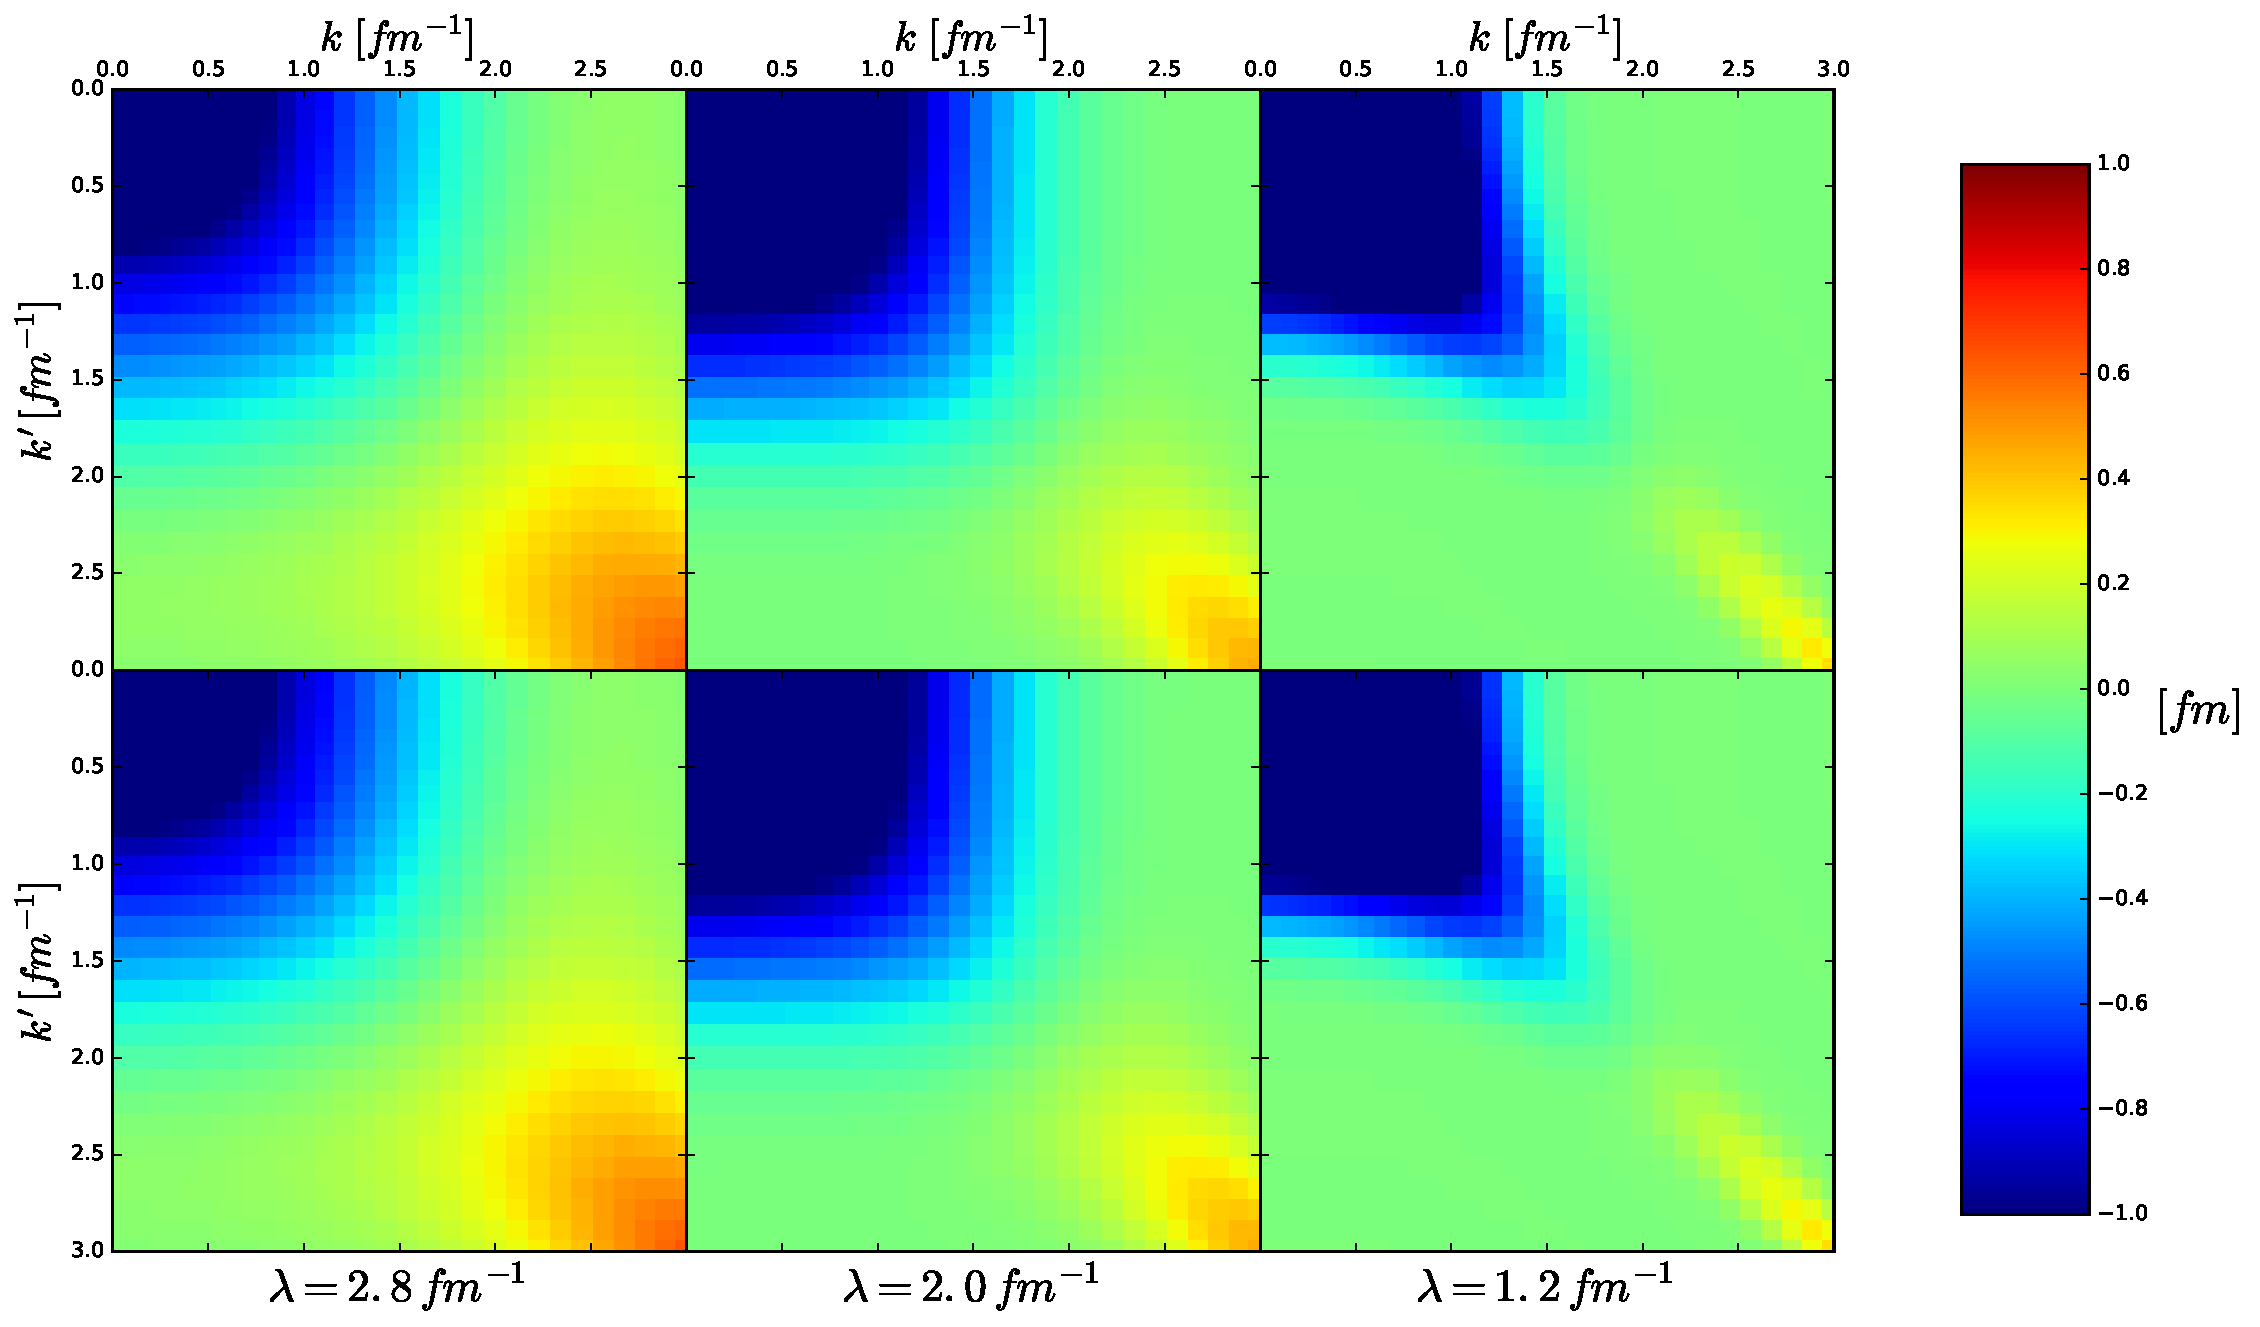
\includegraphics[width=14cm]{srg_contours_Wendt_4}
   \hspace*{0.05\textwidth}%
  \caption{Contour of SRG evolved $V_{\lambda}(k,k')$ with $\Lambda=4.0\,fm^{-1}$, $G=T_{rel}$ (top) and $G=H_{D}$ (bottom) for several values of $\lambda$.}
  \label{fig:srg_contours_Wendt_4}
\end{figure}
%
For $G=T_{rel}$, the spurious, deeply bound state evolves to a point in which it distorts the low-momentum part of $V_{\lambda}(k,k')$. This is seen by comparing the upper left-hand block of the contours between Figures \ref{fig:srg_contours_Wendt_4}, \ref{fig:srg_contours_Wendt_9}, and \ref{fig:srg_contours_Wendt_20}. There is a noticeable difference going from $\Lambda=4.0 \, fm^{-1}$ to $\Lambda=20.0 \, fm^{-1}$, and if one were to calculate the deuteron wave function for instance, the resulting function would differ significantly from the original, unevolved wave function. Thus, the SRG generator corresponding to $G=T_{rel}$ leads to an undesirable evolution for potentials with spurious, deeply bound states. \\
%
\begin{figure}[H]
  \centering
  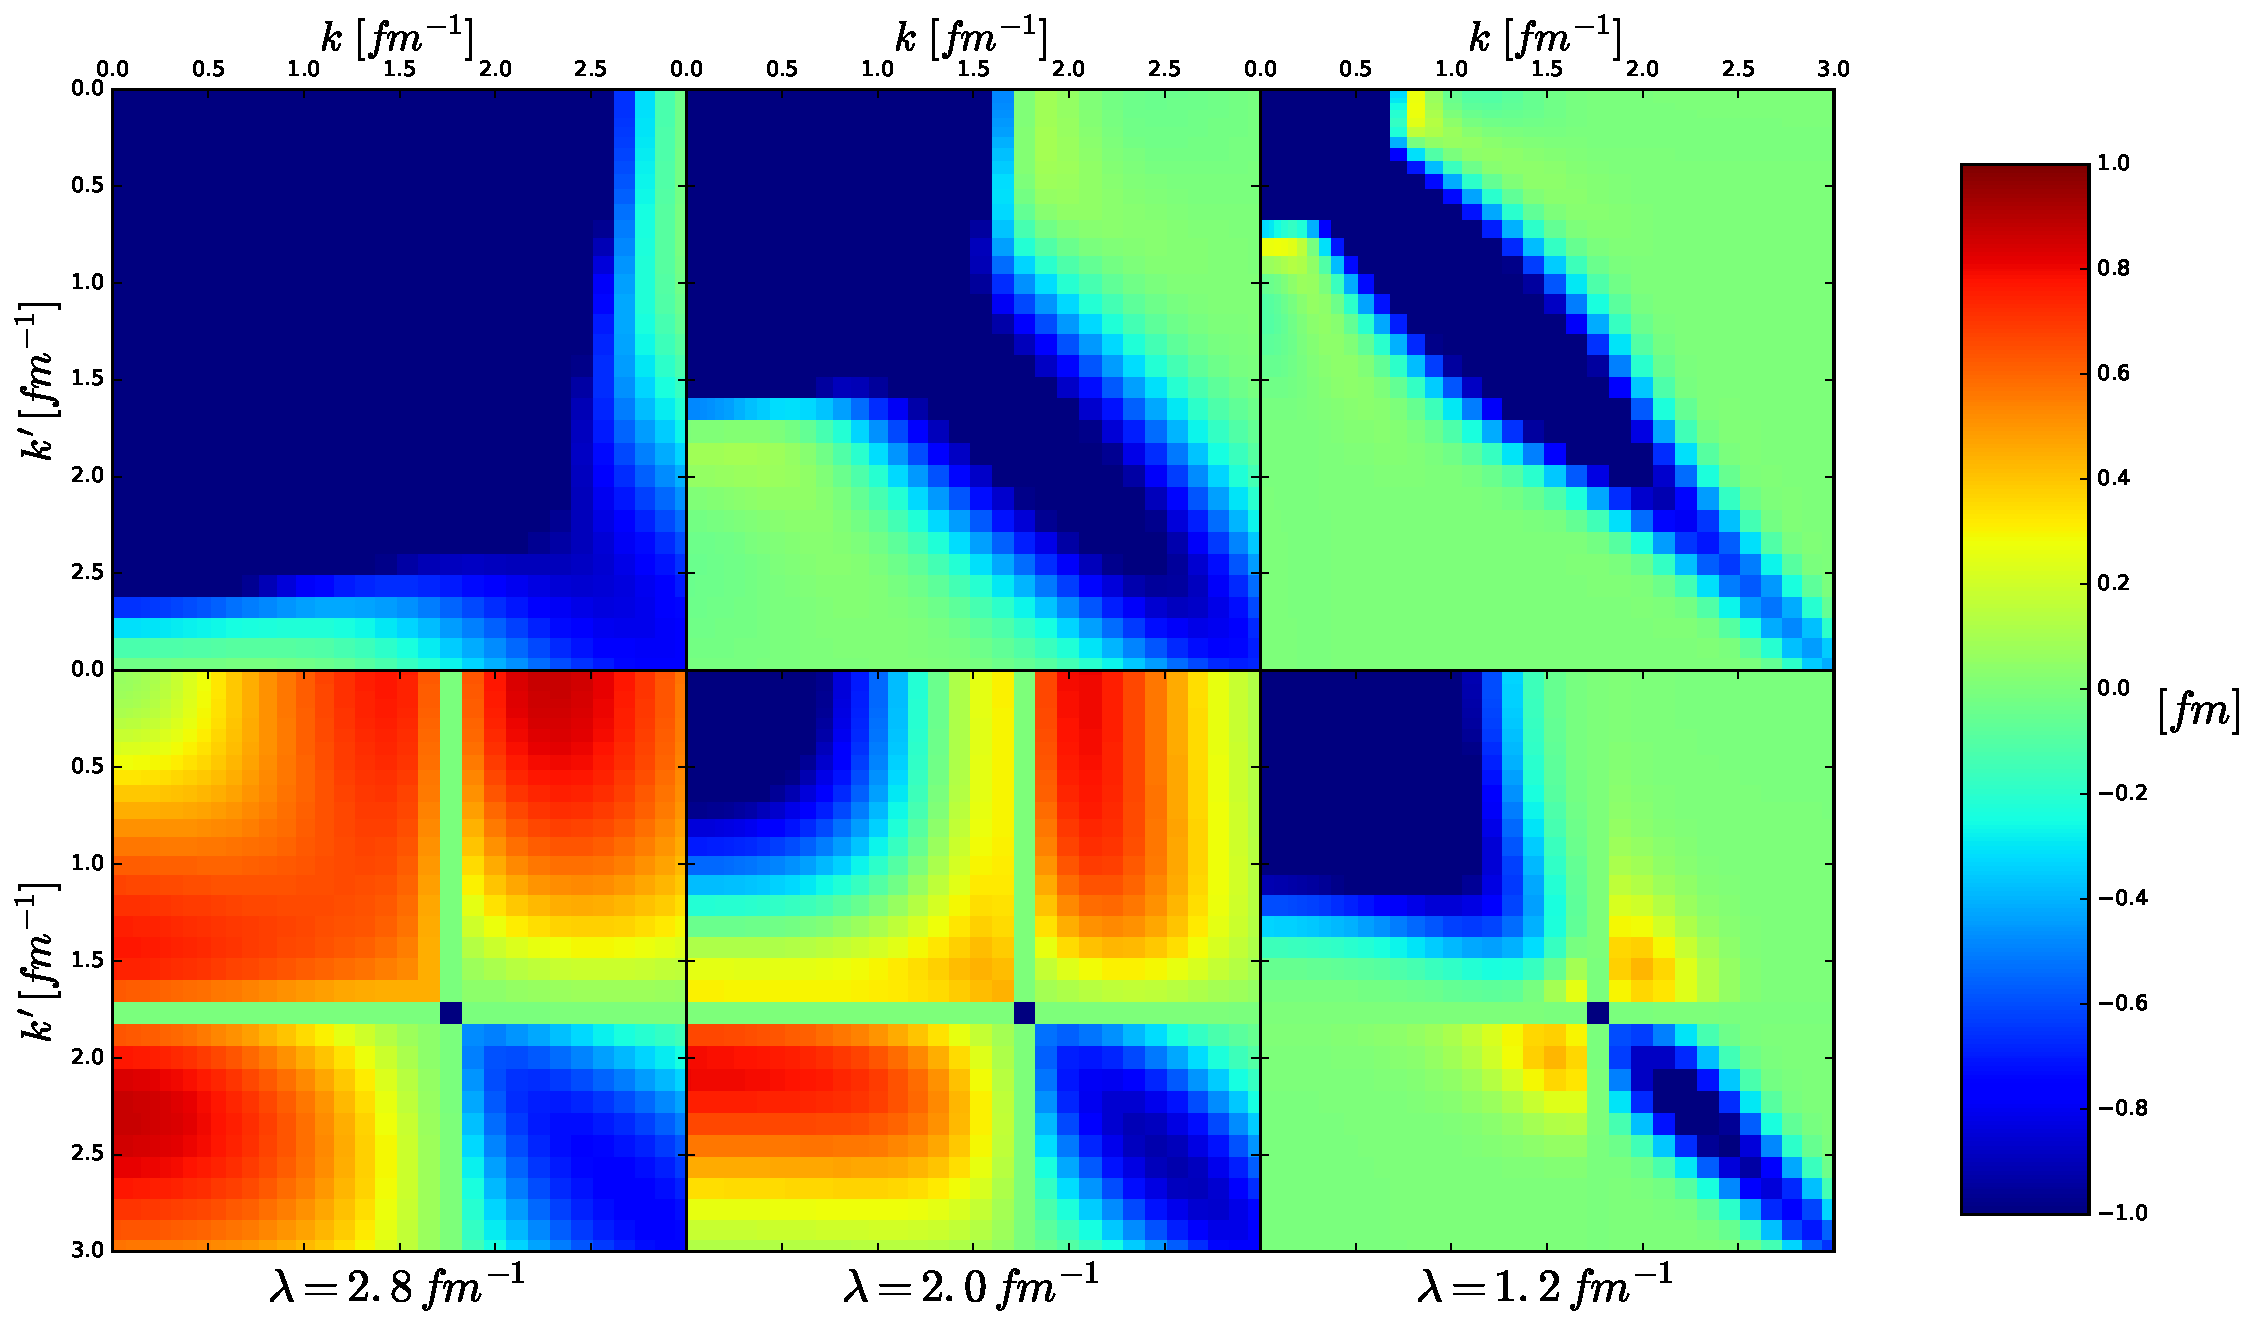
\includegraphics[width=14cm]{srg_contours_Wendt_9}
   \hspace*{0.05\textwidth}%
  \caption{Contour of SRG evolved $V_{\lambda}(k,k')$ with $\Lambda=9.0\,fm^{-1}$, $G=T_{rel}$ (top) and $G=H_{D}$ (bottom) for several values of $\lambda$.}
  \label{fig:srg_contours_Wendt_9}
\end{figure}
%
\begin{figure}[H]
  \centering
  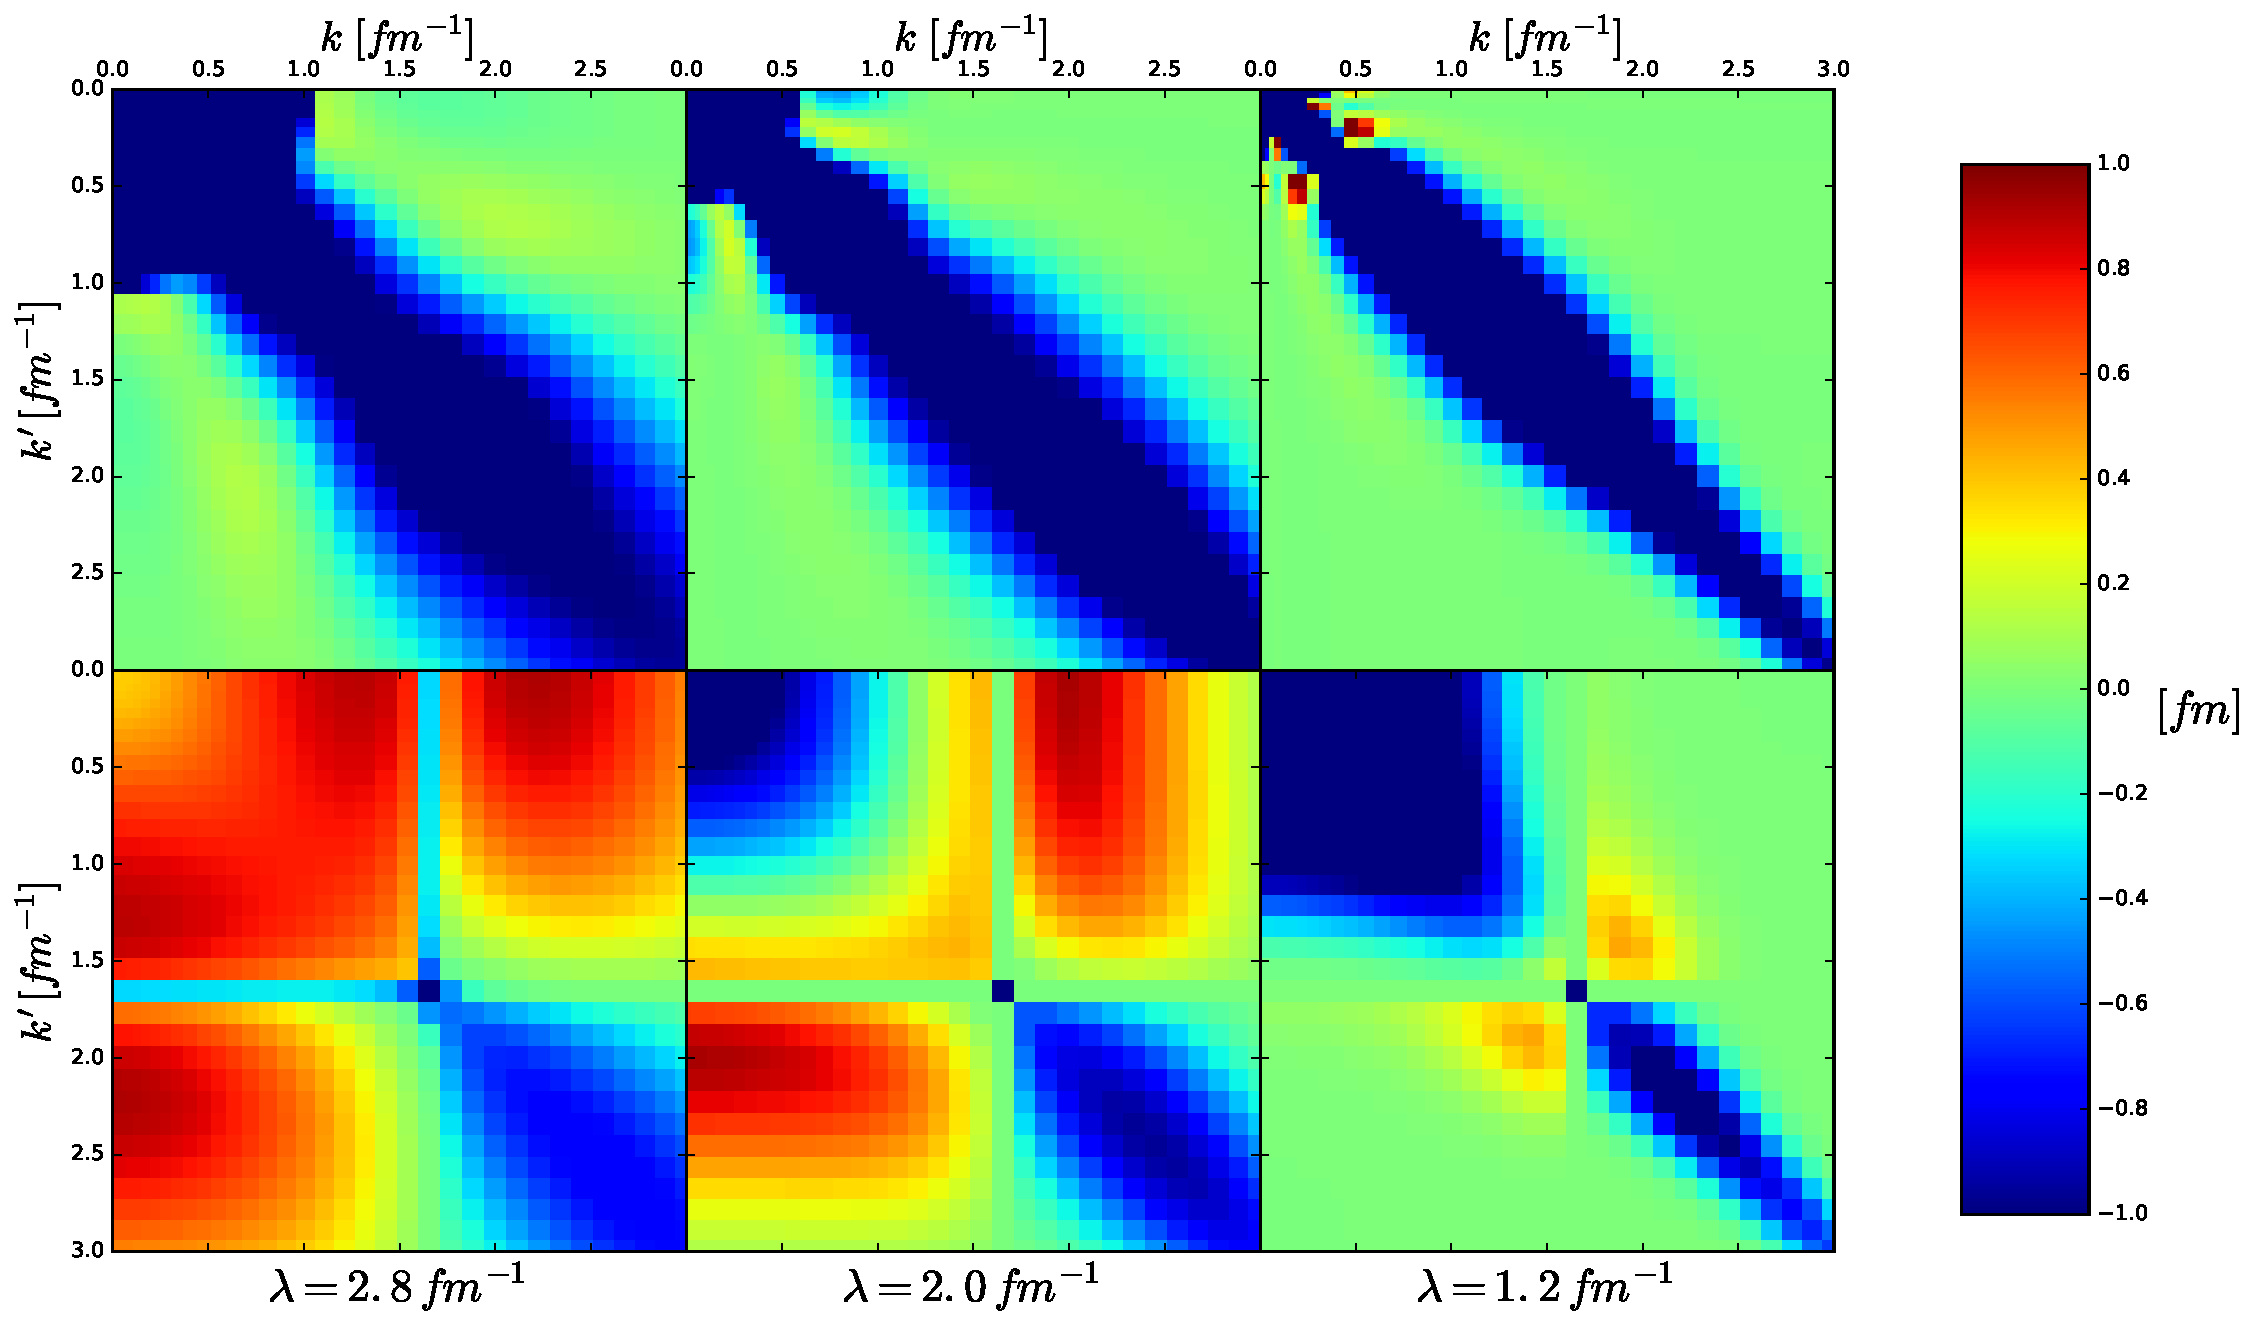
\includegraphics[width=14cm]{srg_contours_Wendt_20}
   \hspace*{0.05\textwidth}%
  \caption{Contour of SRG evolved $V_{\lambda}(k,k')$ with $\Lambda=20.0\,fm^{-1}$, $G=T_{rel}$ (top) and $G=H_{D}$ (bottom) for several values of $\lambda$.}
  \label{fig:srg_contours_Wendt_20}
\end{figure}
%
With the Wegner generator, we see that the spurious, deeply bound state(s) decouple at sufficiently high momentum (meaning it does not affect the low-momentum part of the potential). Once the bound state is decoupled, the SRG evolution drives the potential to the desired band-diagonal form as before. The low-momentum part of the evolved potential is consistent between the three cutoffs unlike with $G=T_{rel}$. This is seen more clearly in Figure \ref{fig:srg_diags_offdiags_Wendt_Wegner}. Therefore, at high cutoffs, the evolution is dependent on the choice of $G$ where the Wegner generator safely evolves the potential by keeping the spurious, deeply bound state(s) outside the low-energy physics. \\
%
\begin{figure}[H]
  \centering
  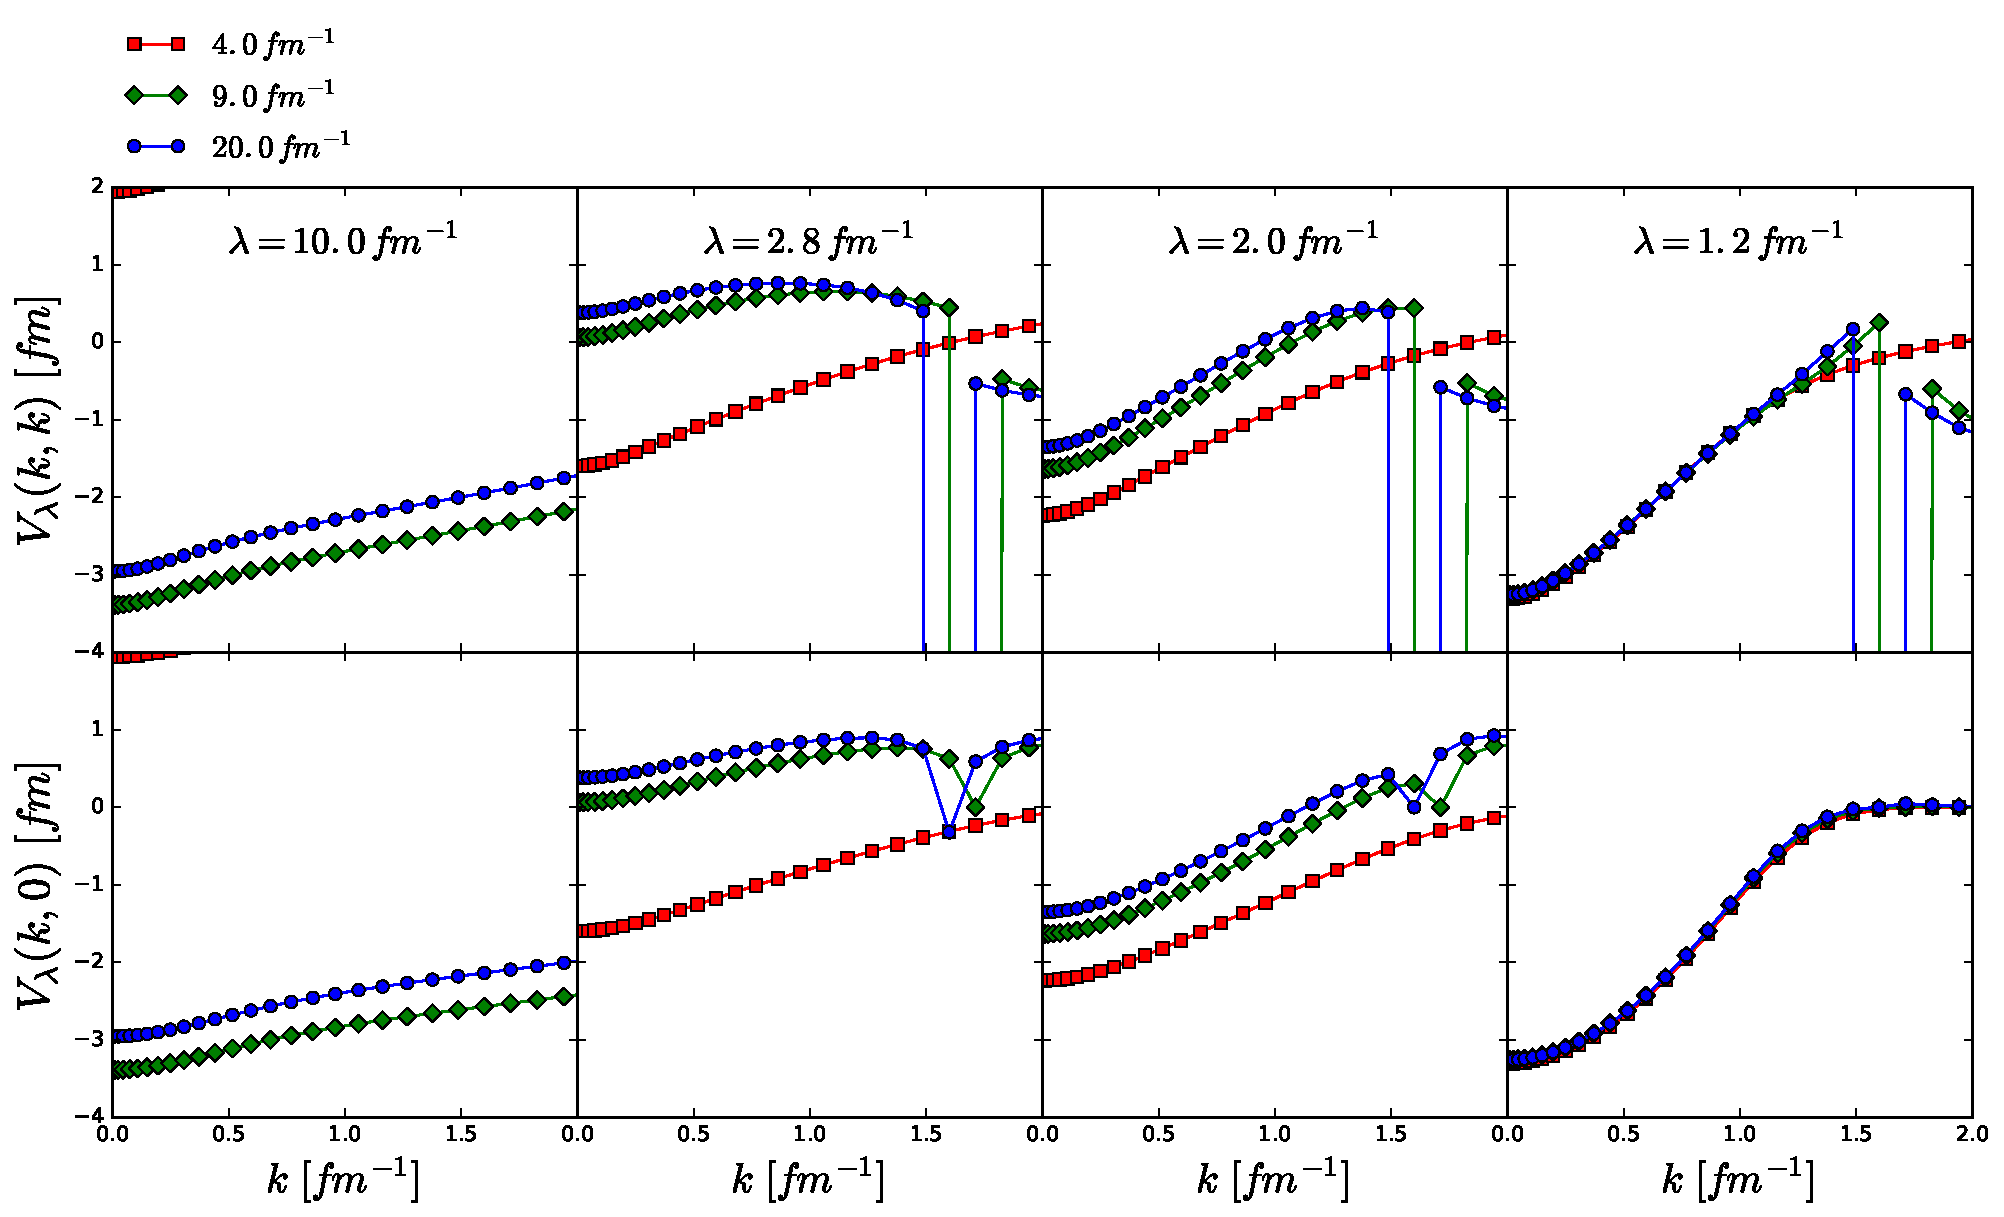
\includegraphics[width=15cm]{srg_diags_offdiags_Wendt_Wegner}
   \hspace*{0.05\textwidth}%
  \caption{Diagonal and off-diagonal matrix elements of SRG evolved $V_{\lambda}(k,k')$ with $G=H_{D}$ for $\Lambda=4.0, \, 9.0, \, 20.0\,fm^{-1}$ and several values of $\lambda$.}
  \label{fig:srg_diags_offdiags_Wendt_Wegner}
\end{figure}
%
Again, it is unusual to see a difference in the SRG evolution going from $G=T_{rel}$ to $G=H_{D}$, but the presence of spurious, deeply bound states significantly affects the SRG procedure. In practice, these potentials at high cutoffs are not very useful; however, they do offer a nice test case for the Magnus expansion given their sensitivity to SRG evolution. It is critical that the Magnus implementation matches the typical SRG approach if one is to understand the IMSRG intruder state problem using the Magnus expansion. In the following section, we compare results between the Magnus expansion and the typical SRG approach for these potentials. \\
%
\begin{figure}[H]
  \centering
  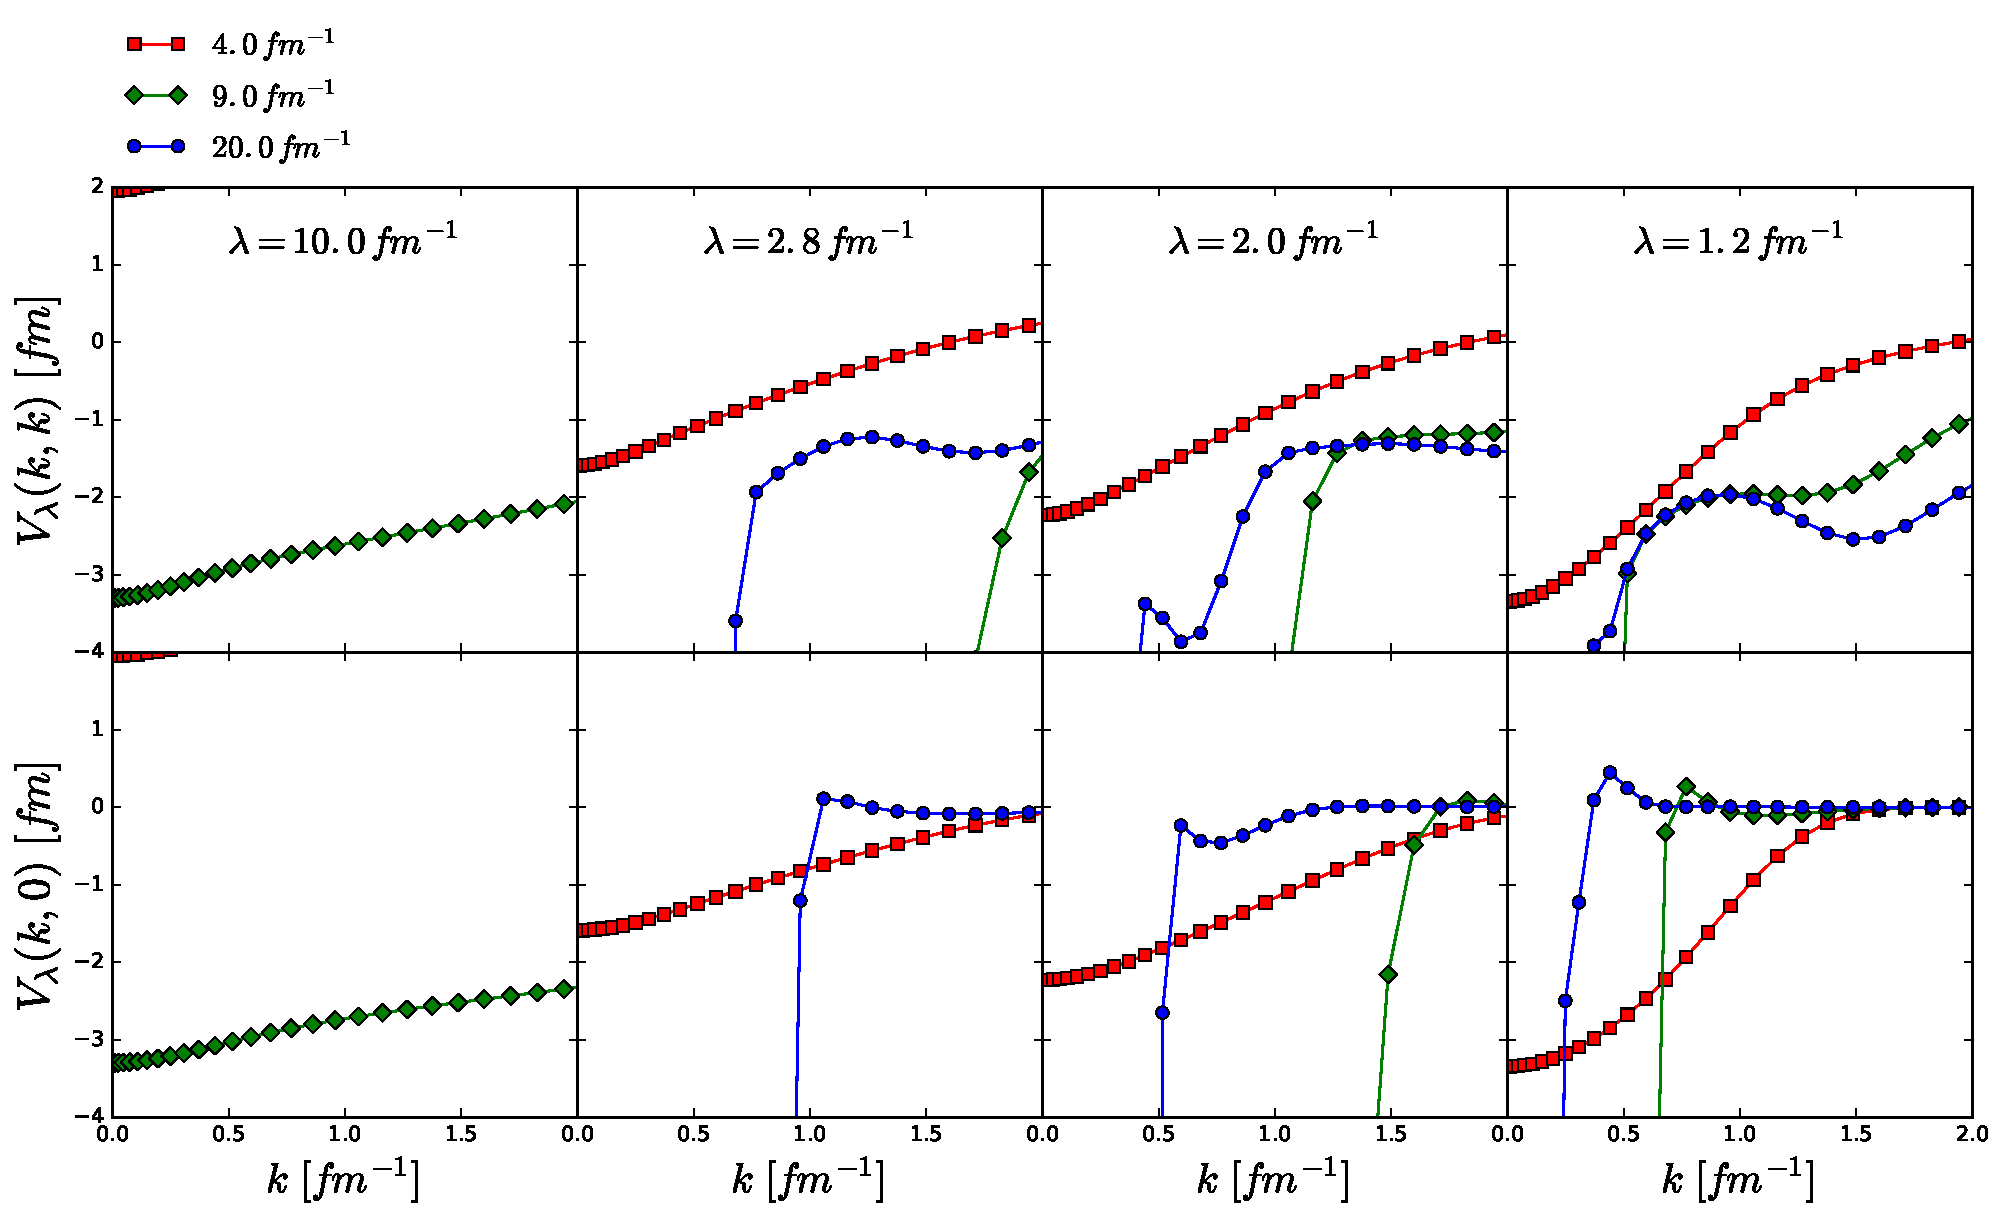
\includegraphics[width=15cm]{srg_diags_offdiags_Wendt_Wilson}
   \hspace*{0.05\textwidth}%
  \caption{Diagonal and off-diagonal matrix elements of SRG evolved $V_{\lambda}(k,k')$ with $G=T_{rel}$ for $\Lambda=4.0, \, 9.0, \, 20.0\,fm^{-1}$ and several values of $\lambda$.}
  \label{fig:srg_diags_offdiags_Wendt_Wilson}
\end{figure}

%%%%%%%%%%%%%%%%%%%%%%%%%%%%%%%%%%%%%%%%%%%%%%%%%%%%%%%%%%%%%%%%%%%%%%%%%
\section{The Magnus expansion at high $\Lambda$}
\label{sec:magnus_high_lambda}

% .....................................................................................................................................................................................................................................
\subsection{Evolved potentials}

In this subsection, we compare the evolved potentials, $V_{\lambda}(k,k')$, for the typical SRG approach and the Magnus implementation. For all figures presented in this subsection, the first-order Euler method with a fixed step-size, $ds=10^{-5}$, was used to solve Eq. (\ref{eq:magnus_omega}) in the Magnus implementation. For the most part, there is no sensitivity to the step-size, only that it has to be chosen such that ``enough" steps are taken in evolving $V_{\lambda}(k,k')$ (for instance, at $\lambda=10.0 \, fm^{-1}$ we set $ds=10^{-6}$ to get good agreement with the standard SRG approach since $ds=10^{-5}$ would only result in a total of 12 steps in $s$). However, the evolution of $V_{\lambda}(k,k')$ does depend significantly on the truncation of the Magnus series, $k_{max}$, particularly at higher cutoffs in $\Lambda$. Here $k_{max}$ represents the last term included in the Magnus series in numerically solving Eq. (\ref{eq:magnus_omega}).
%
\begin{figure}[H]
  \centering
  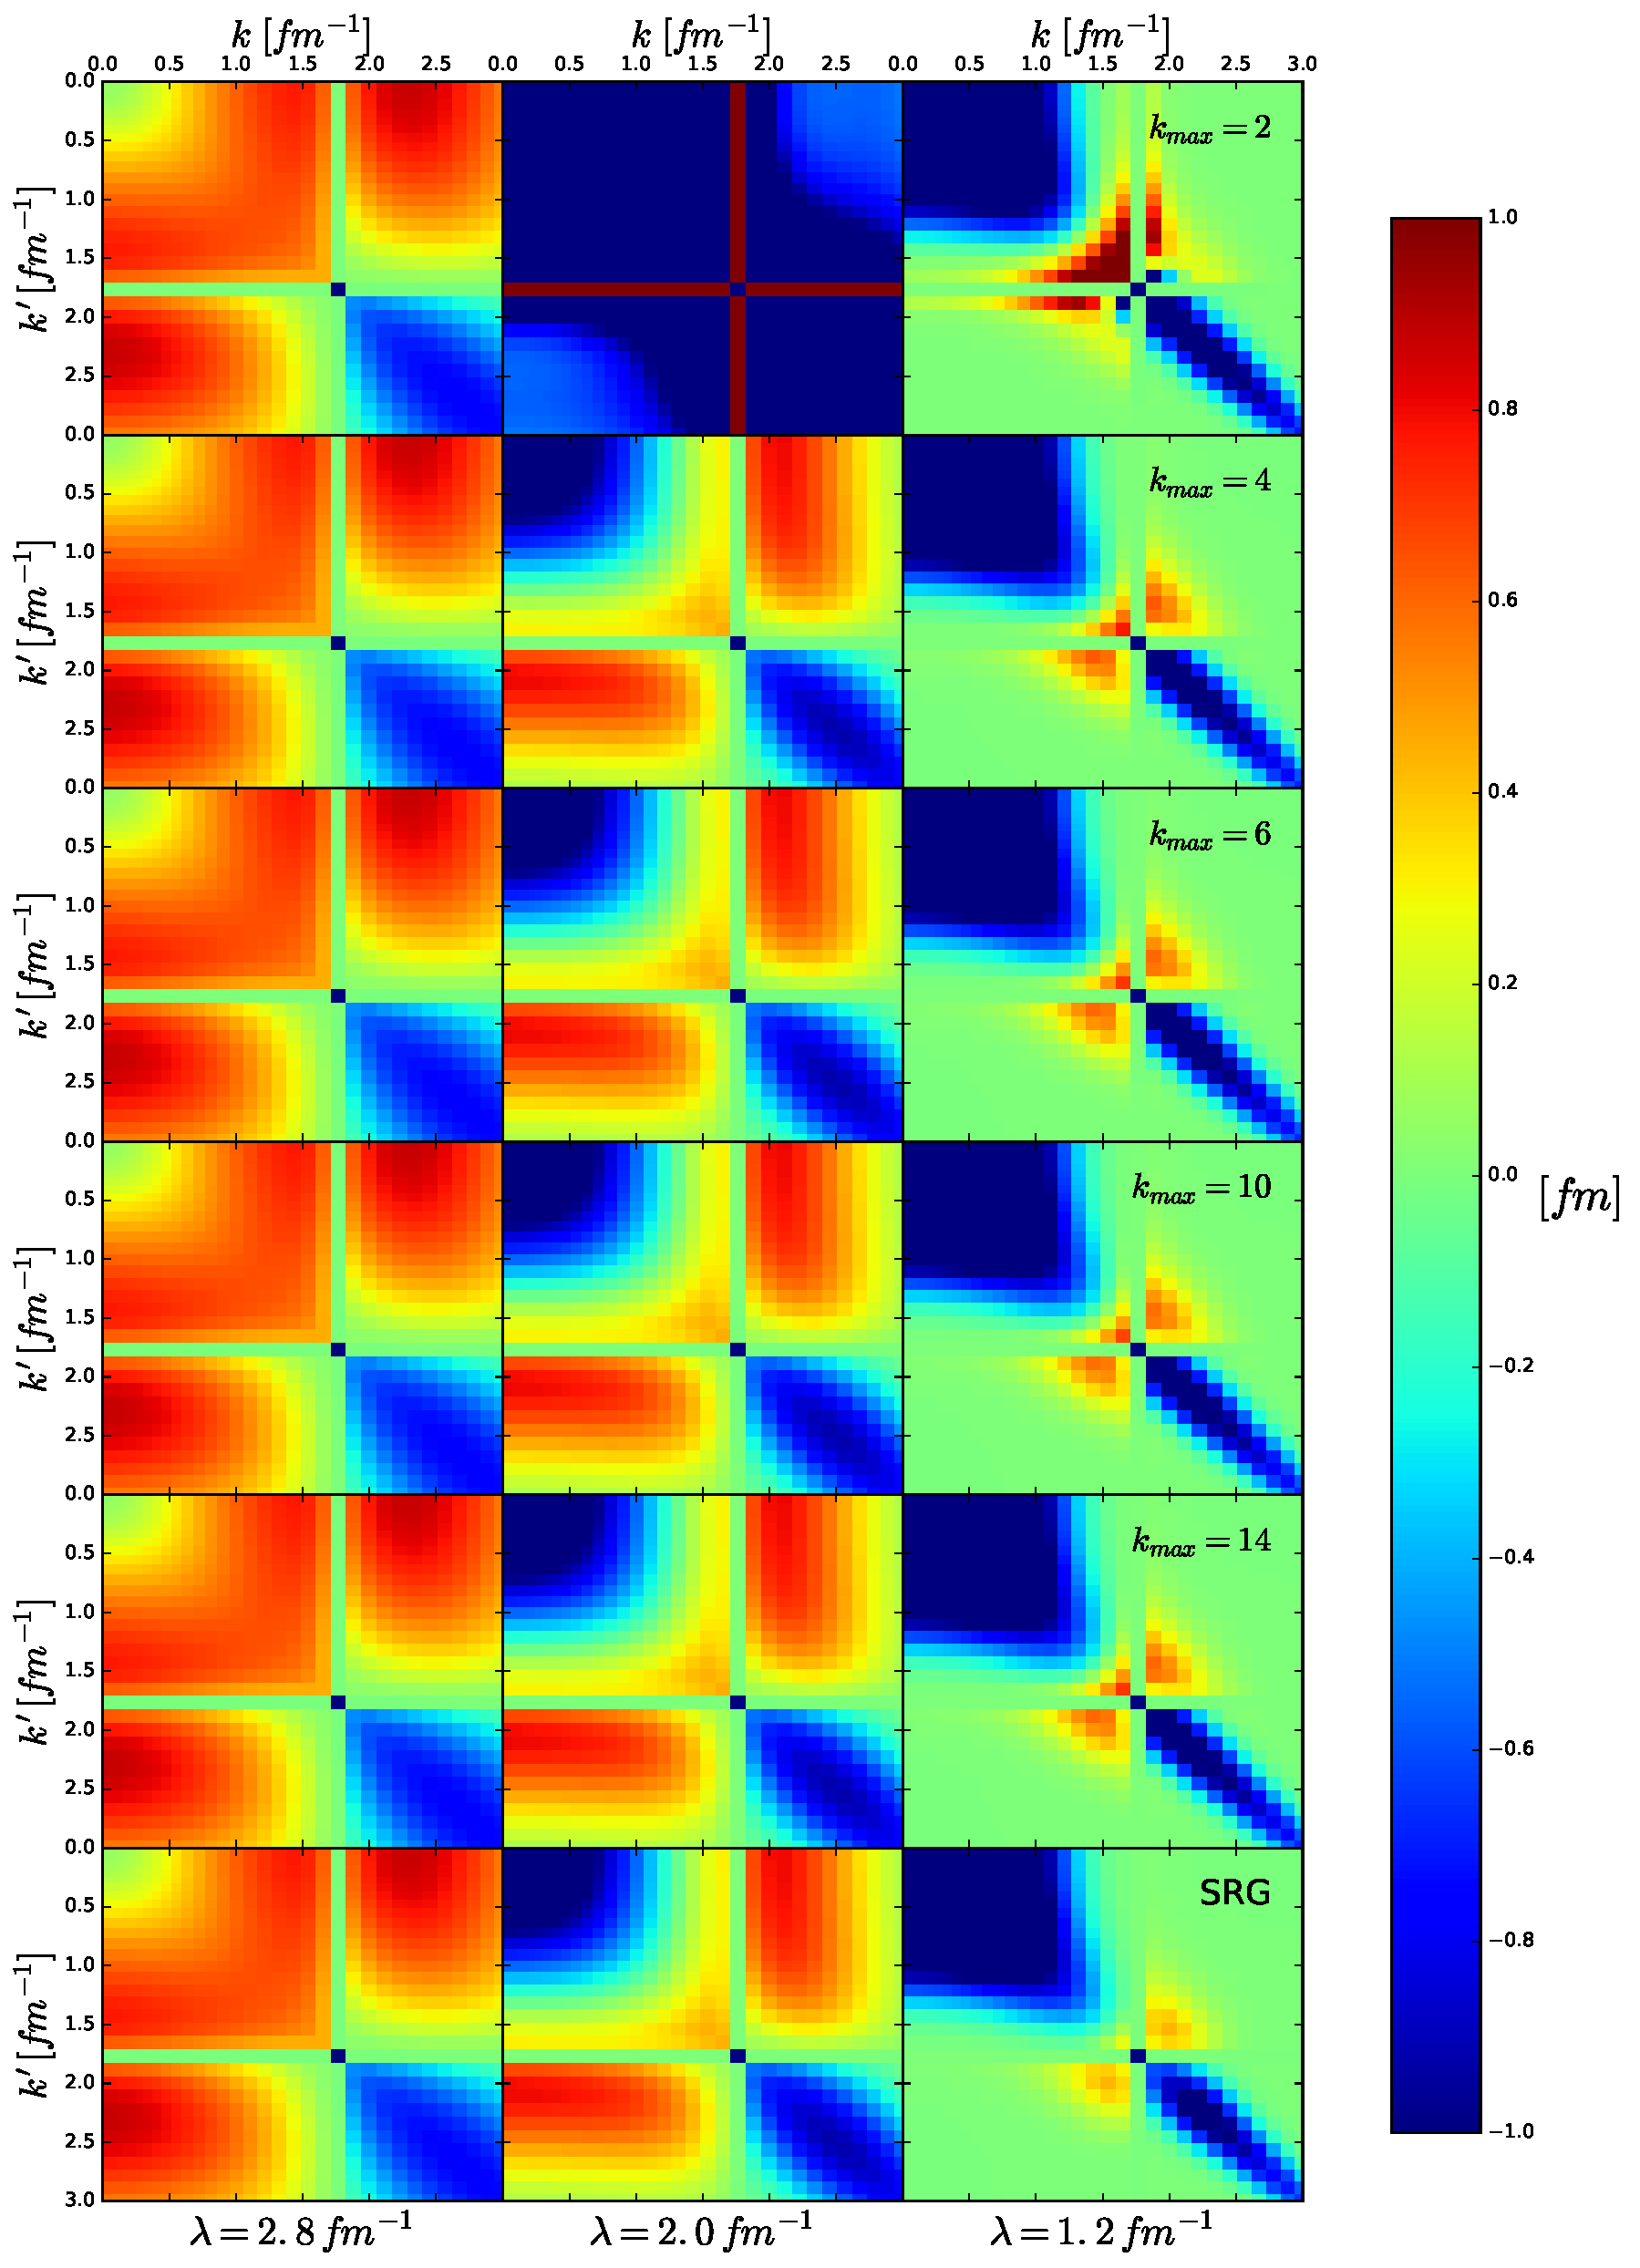
\includegraphics[width=15cm]{mag_contours_Wendt_9_Wegner}
   \hspace*{0.05\textwidth}%
  \caption{Contour of evolved $V_{\lambda}(k,k')$ with $\Lambda=9.0\,fm^{-1}$ and $G=H_{D}$ for several values of $\lambda$. Each row corresponds to a different truncation in the Magnus expansion (2, 4, 6, 10, 14) with the last row being the SRG result.}
  \label{fig:mag_contours_Wendt_9_Wegner}
\end{figure}
%
\begin{figure}[H]
  \centering
  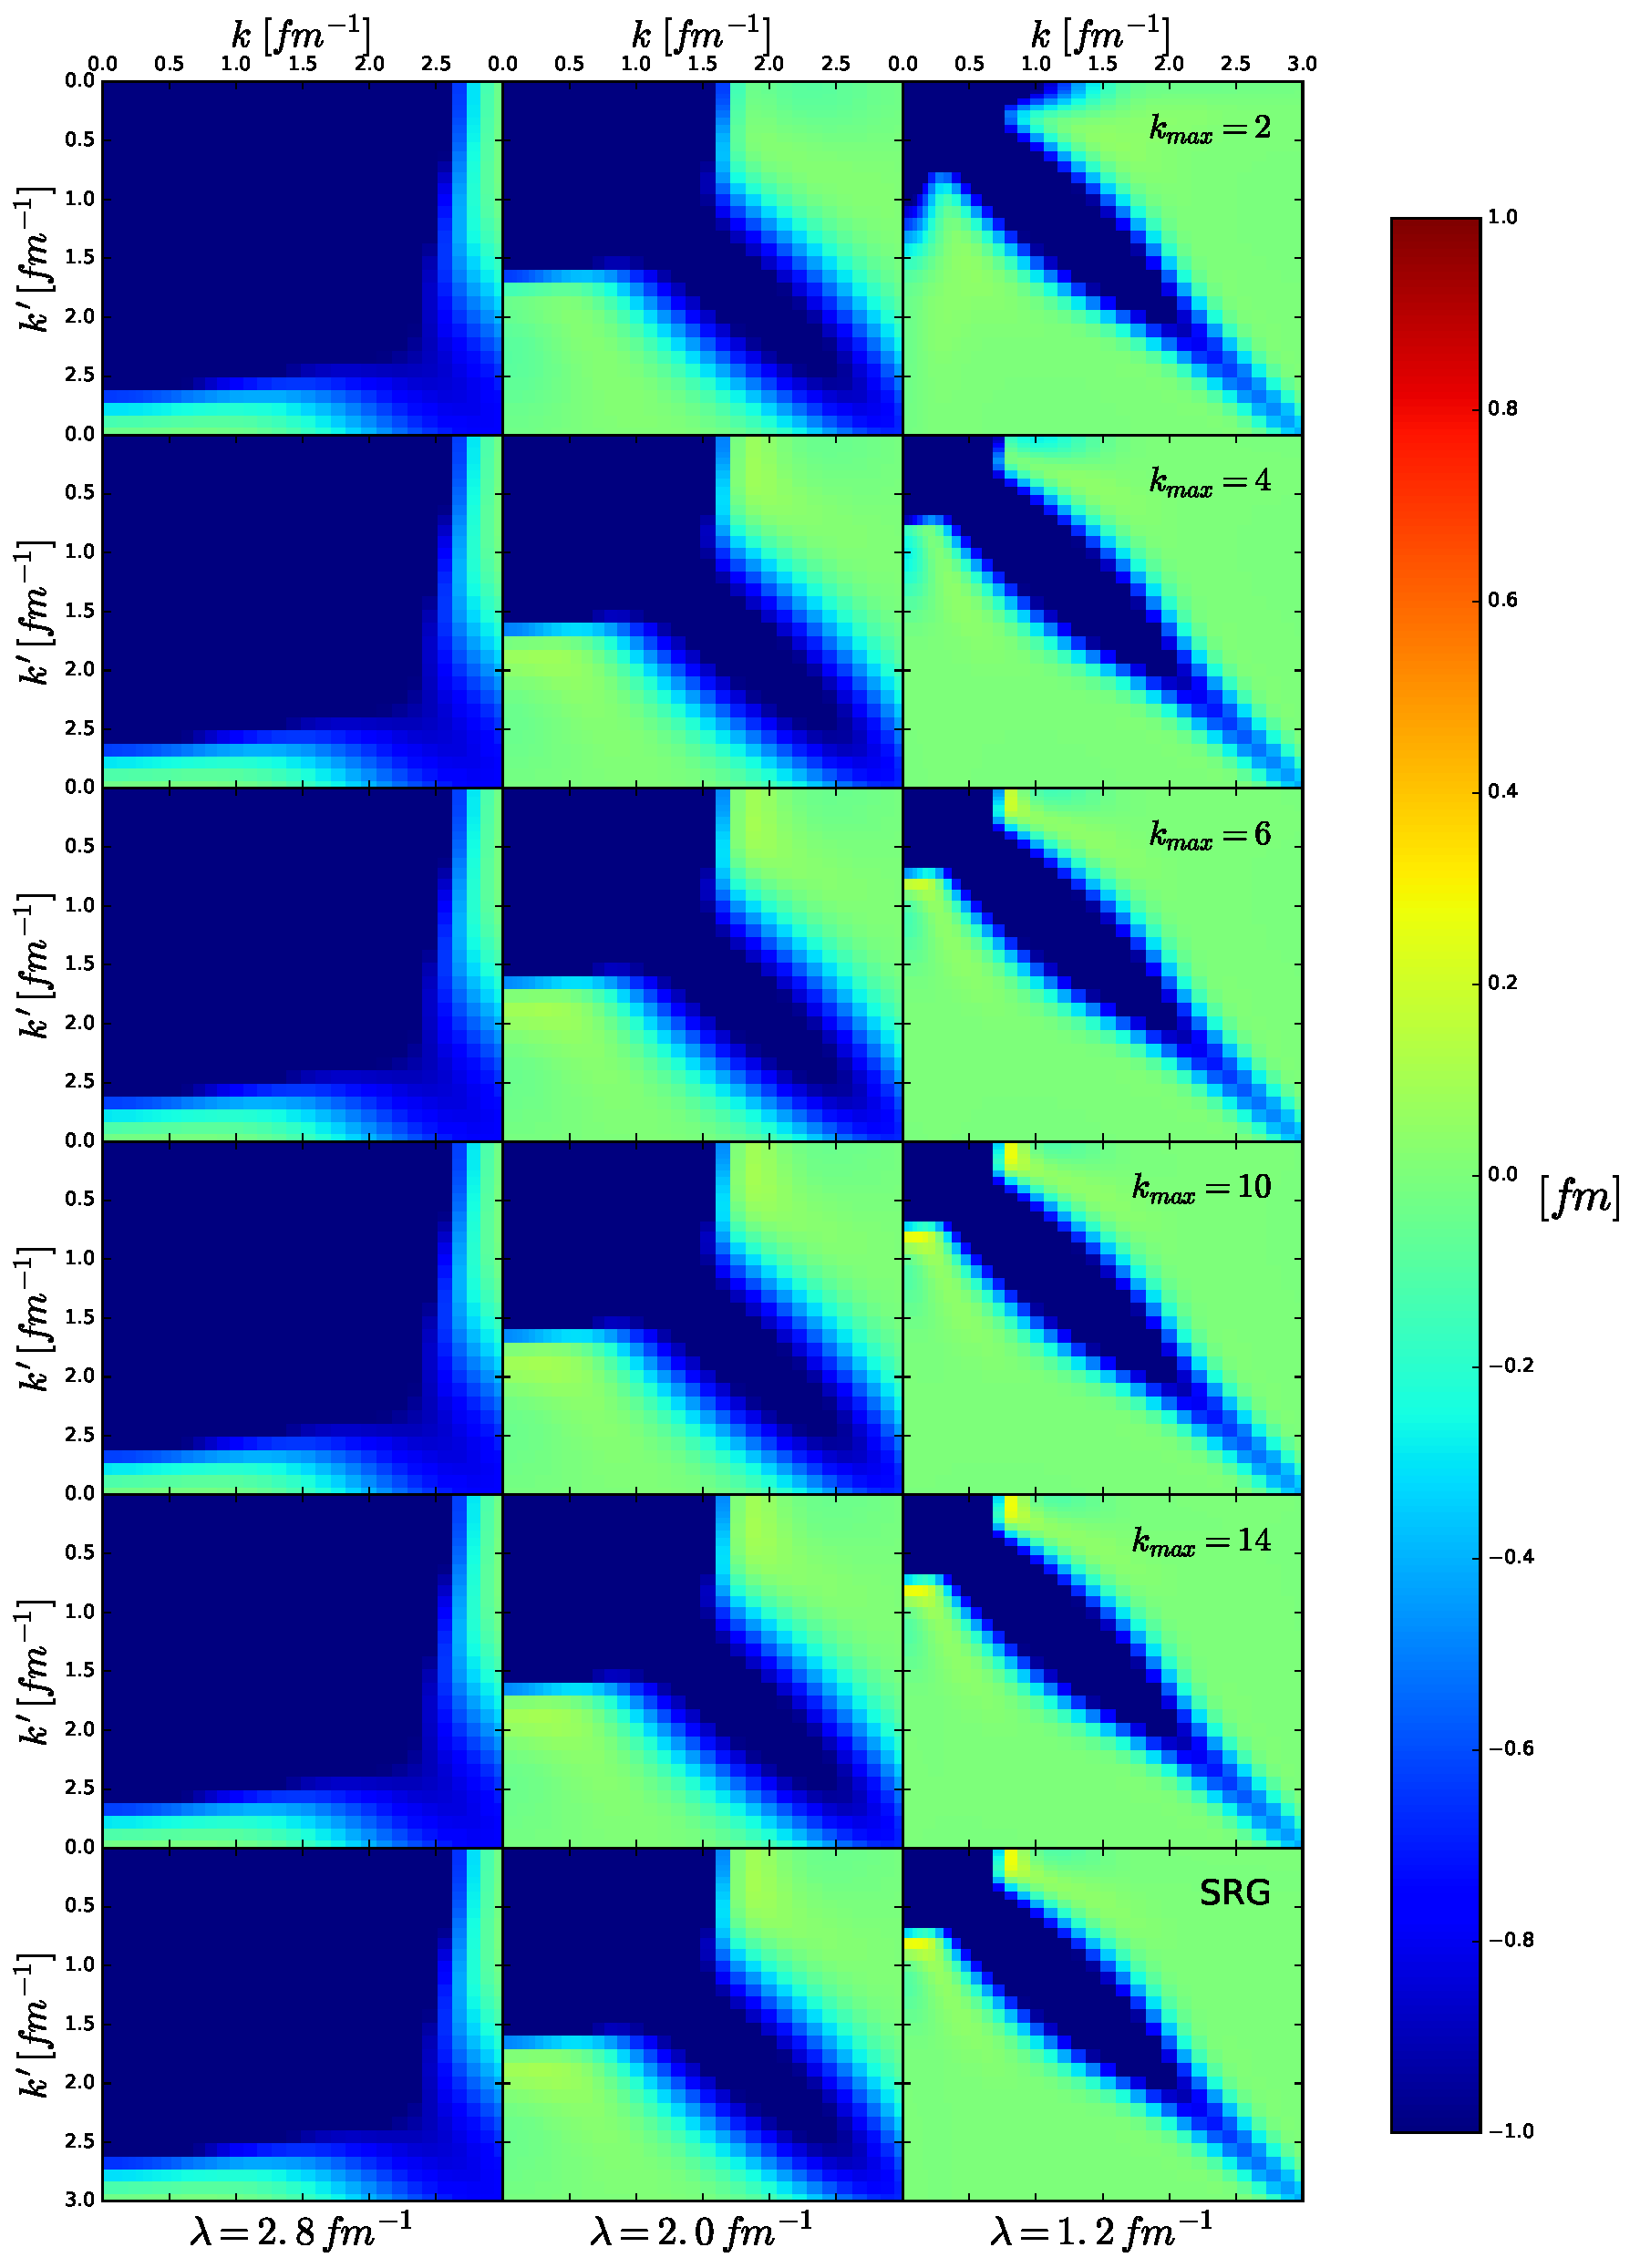
\includegraphics[width=15cm]{mag_contours_Wendt_9_Wilson}
   \hspace*{0.05\textwidth}%
  \caption{Contour of evolved $V_{\lambda}(k,k')$ with $\Lambda=9.0\,fm^{-1}$ and $G=T_{rel}$ for several values of $\lambda$. Each row corresponds to a different truncation in the Magnus expansion (2, 4, 6, 10, 14) with the last row being the SRG result.}
  \label{fig:mag_contours_Wendt_9_Wilson}
\end{figure}
%
In Figure \ref{fig:mag_contours_Wendt_9_Wegner} we show contours of the evolving potential for $\Lambda=9.0 \, fm^{-1}$ with the Wegner generator. This figure compares the Magnus implementation at several truncations to the SRG result (bottom row). Notice the large off-diagonal values in $V_{\lambda}(k,k')$ at $\lambda=2.0 \, fm^{-1}$ for $k_{max}=2$. This illustrates the point that using the Magnus expansion with a low truncation can lead to an undesirable flow. Taking $k_{max}$ to higher values reproduces the SRG result to moderate accuracy. An important piece to notice in Figure \ref{fig:mag_contours_Wendt_9_Wegner} is that the Magnus reproduces the decoupling of the spurious, deeply bound state at all values of $k_{max}$ as in the SRG approach. At $\lambda=1.2 \, fm^{-1}$ there is a slight difference in the evolved potential near the decoupled spurious bound state, although the low-momentum block is nearly identical.
%
\begin{figure}[H]
  \centering
  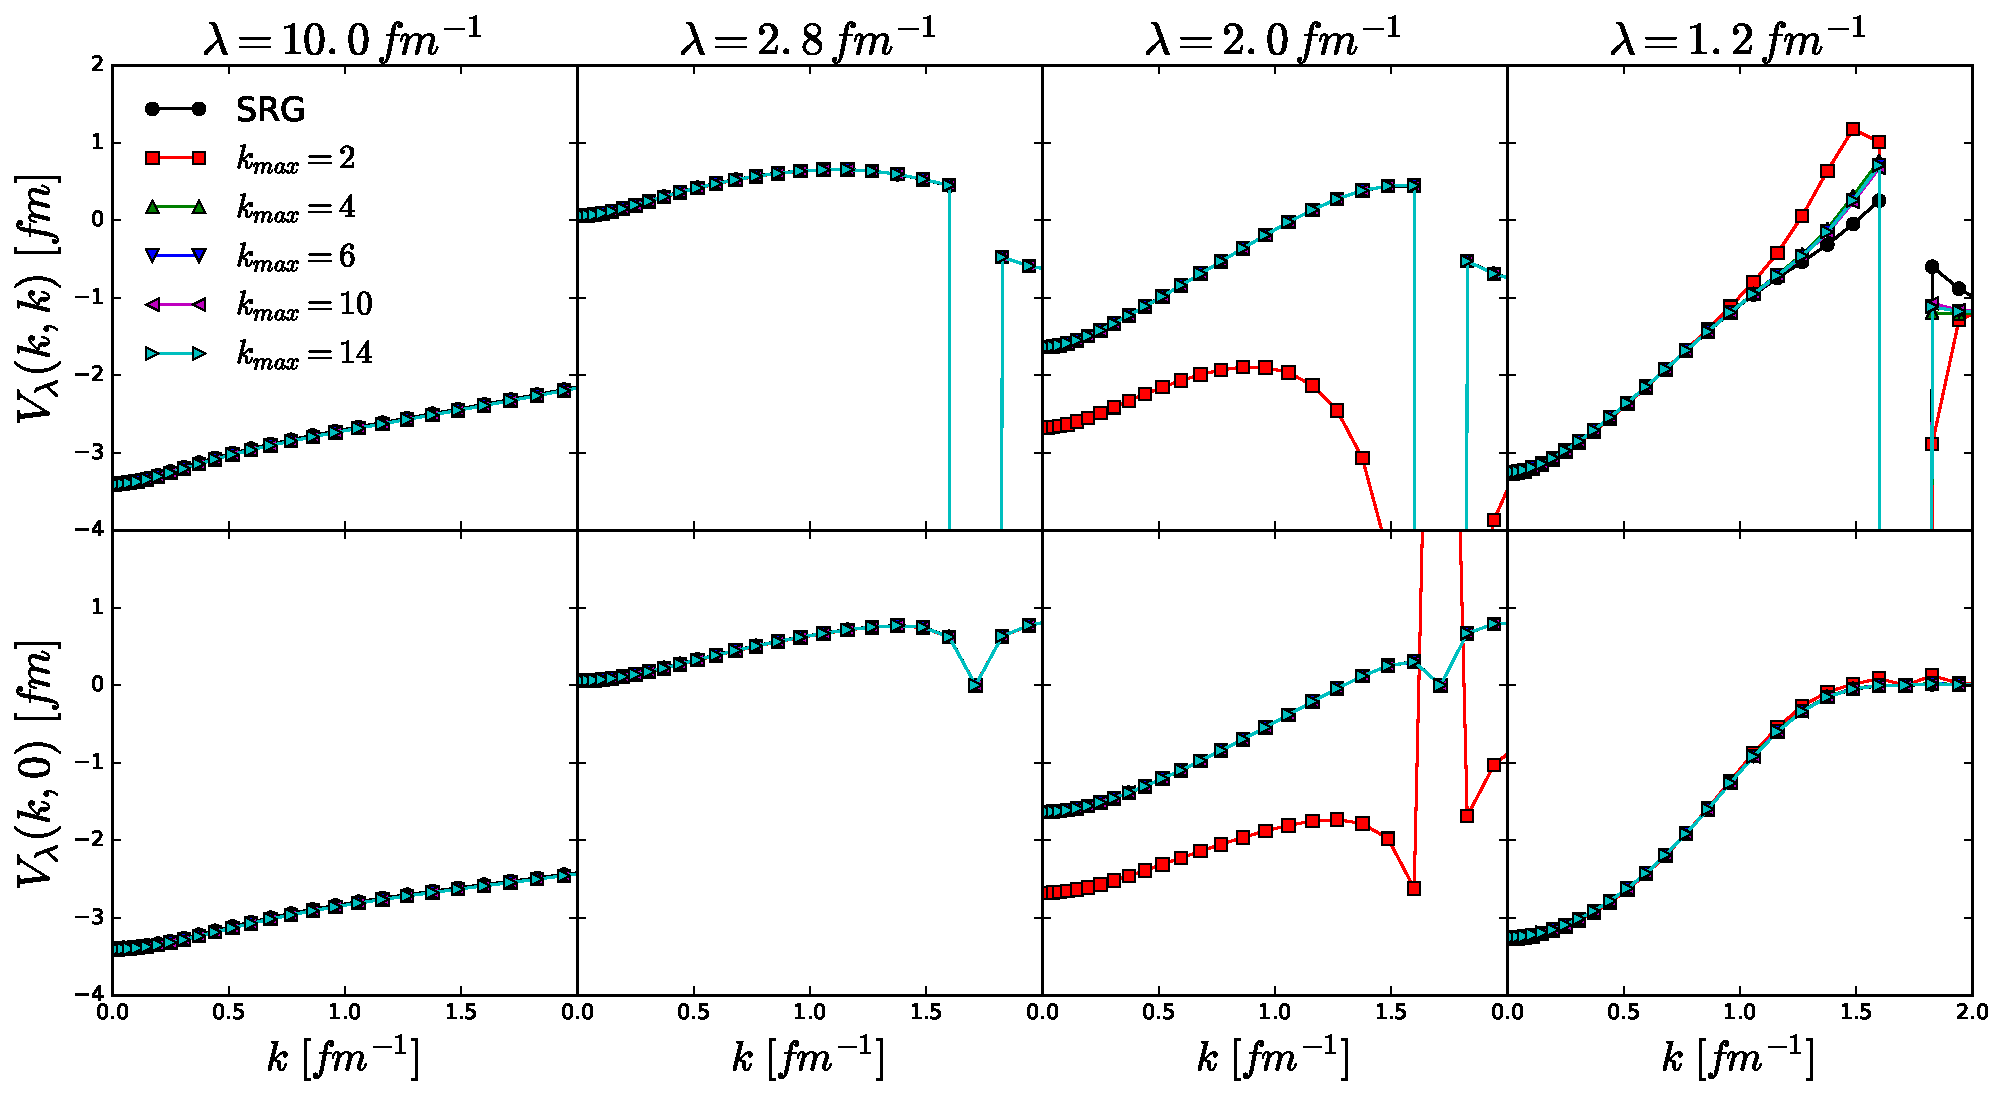
\includegraphics[width=15cm]{mag_diags_offdiags_Wendt_9_Wegner}
   \hspace*{0.05\textwidth}%
  \caption{Diagonal and off-diagonal matrix elements of evolved $V_{\lambda}(k,k')$ with $G=H_{D}$ and $\Lambda=9.0 \, fm^{-1}$ for several values of $\lambda$ and $k_{max}$ compared to the SRG result.}
  \label{fig:mag_diags_offdiags_Wendt_9_Wegner}
\end{figure}
%
Figure \ref{fig:mag_contours_Wendt_9_Wilson} shows the result for $G=T_{rel}$. Again, we see that the Magnus implementation reproduces the SRG generator sensitivity, in particular, how the spurious, deeply bound state is decoupled. This reinforces the conclusion that the Wegner generator safely evolves the potential whereas the $G=T_{rel}$ choice does not. The higher truncations in Figure \ref{fig:mag_contours_Wendt_9_Wilson} are in very good agreement with the SRG result. This can be seen more quantitatively in Figures \ref{fig:mag_diags_offdiags_Wendt_9_Wegner} and \ref{fig:mag_diags_offdiags_Wendt_9_Wilson}. These figures show the diagonal and off-diagonal elements of $V_{\lambda}(k,k')$ for several values of $k_{max}$ compared to the SRG result. We see the decoupling of the spurious bound state in the upper three panels of Figure \ref{fig:mag_diags_offdiags_Wendt_9_Wegner} where the curve dips down to large negative values at $k \approx 1.75 \, fm^{-1}$.
%
\begin{figure}[H]
  \centering
  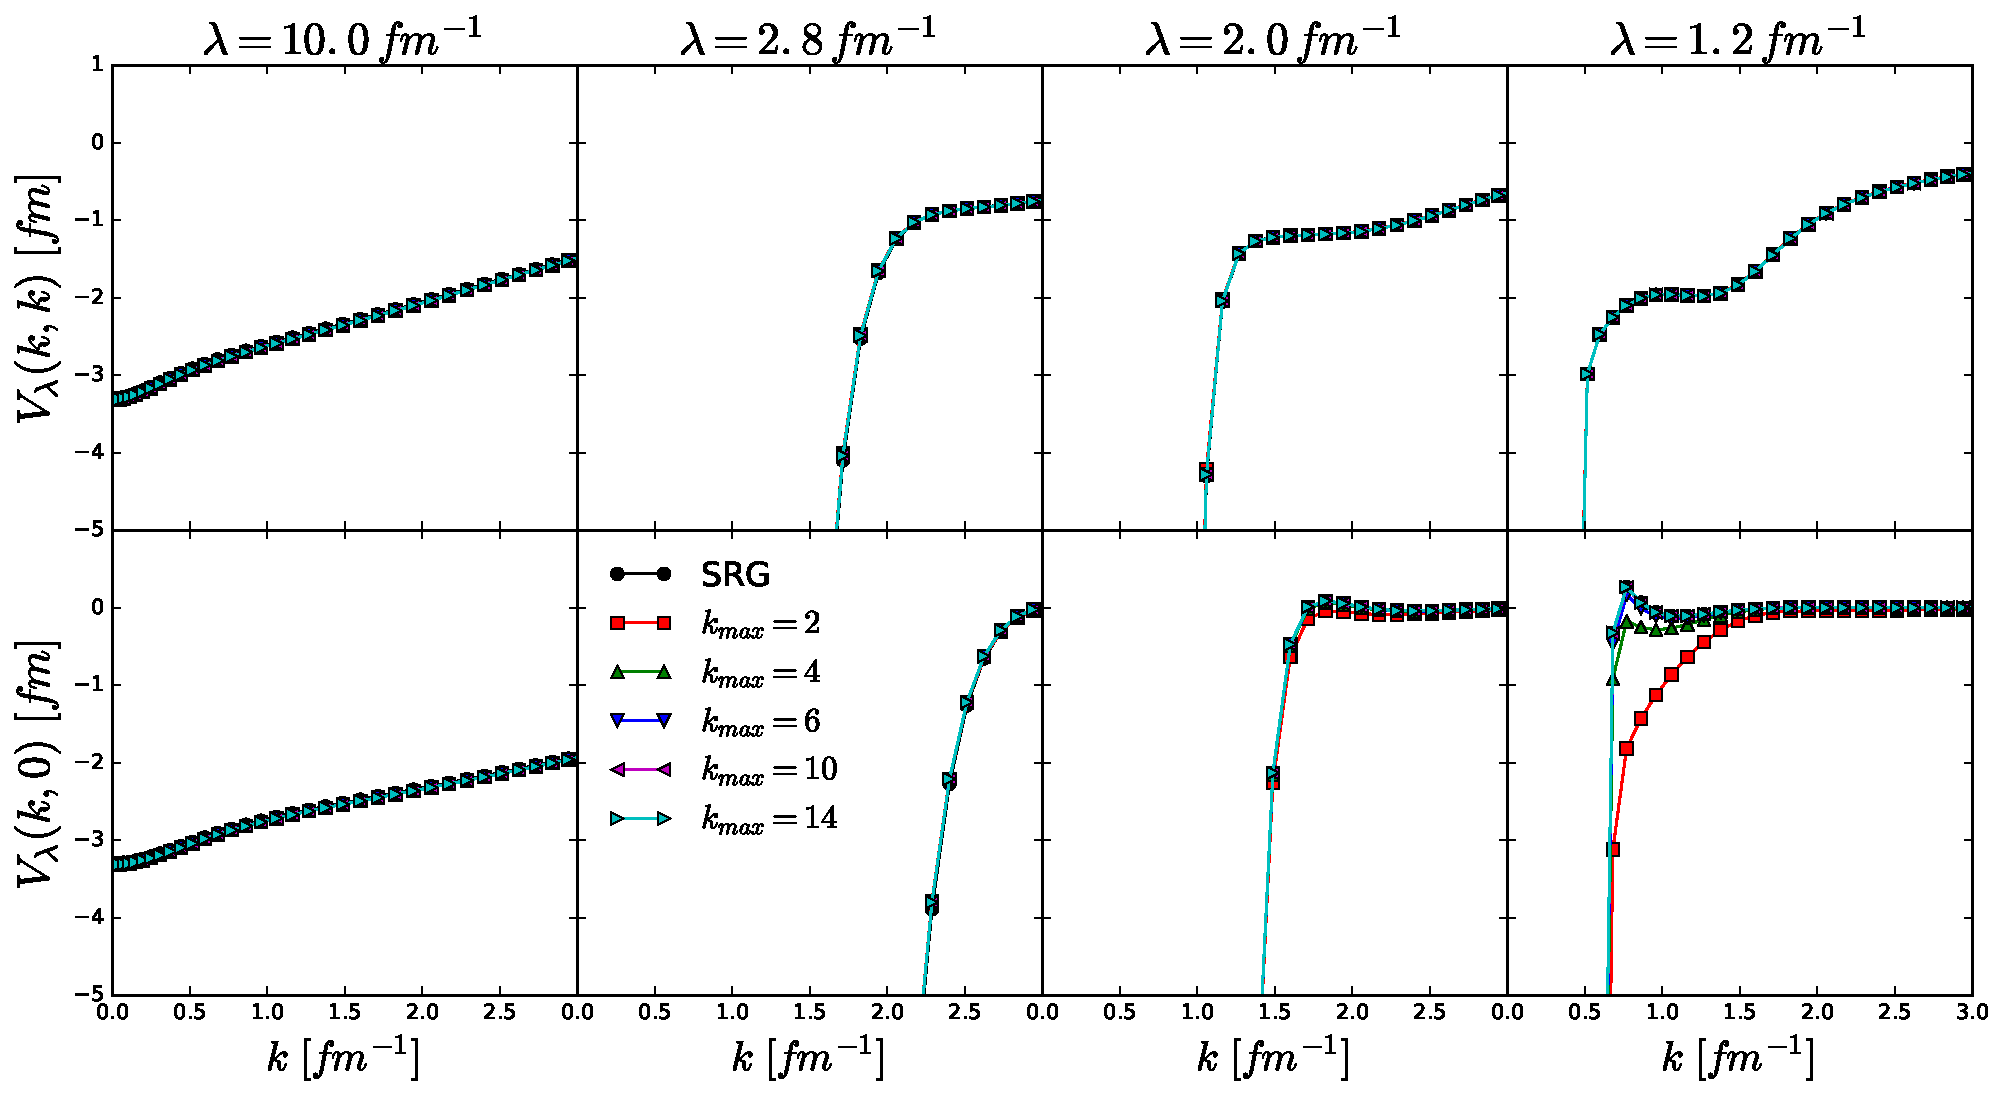
\includegraphics[width=15cm]{mag_diags_offdiags_Wendt_9_Wilson}
   \hspace*{0.05\textwidth}%
  \caption{Diagonal and off-diagonal matrix elements of evolved $V_{\lambda}(k,k')$ with $G=T_{rel}$ and $\Lambda=9.0 \, fm^{-1}$ for several values of $\lambda$ and $k_{max}$ compared to the SRG result.}
  \label{fig:mag_diags_offdiags_Wendt_9_Wilson}
\end{figure}
%
\begin{figure}[H]
  \centering
  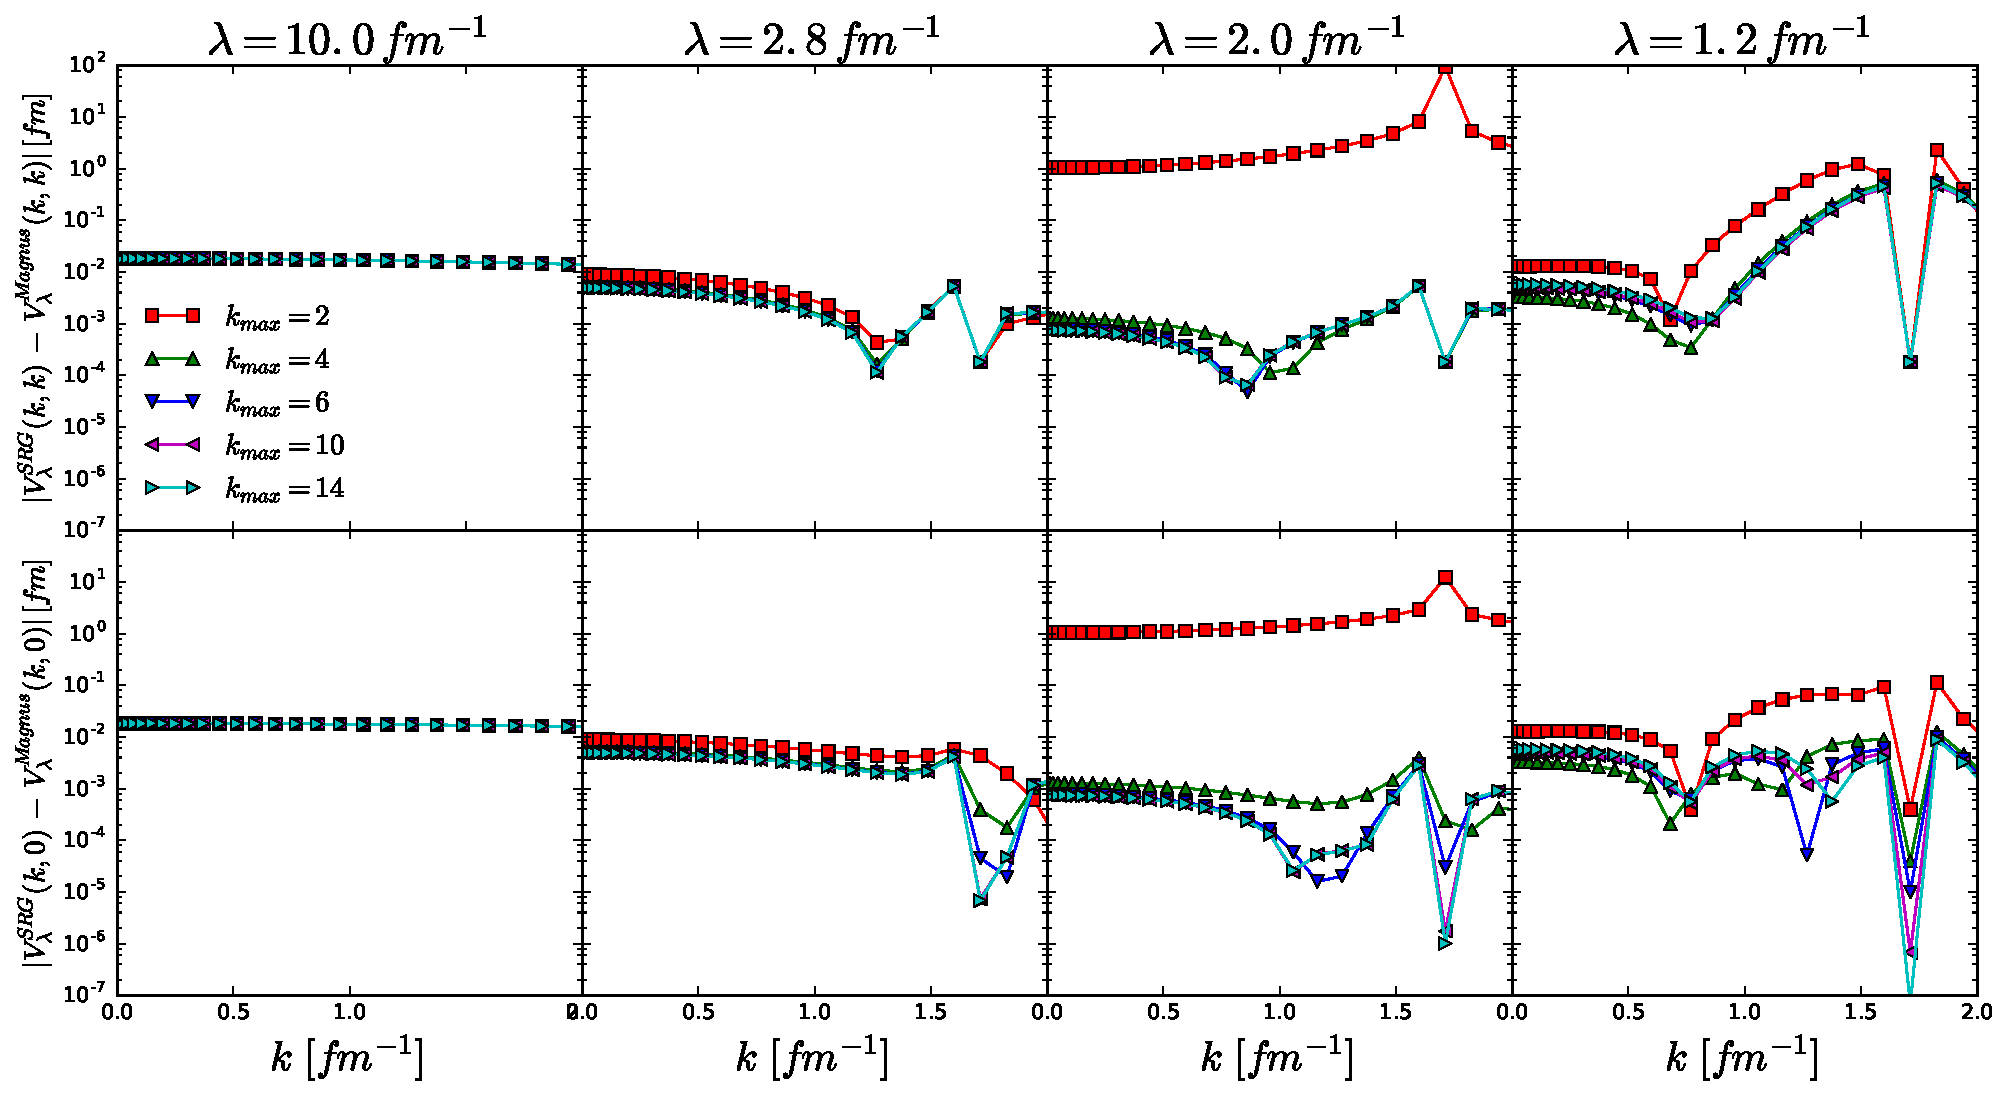
\includegraphics[width=15cm]{mag_diff_Wendt_9_Wegner}
   \hspace*{0.05\textwidth}%
  \caption{Difference in the diagonal and off-diagonal matrix elements of evolved $V_{\lambda}(k,k')$ with $G=H_D$ and $\Lambda=9.0 \, fm^{-1}$ for several values of $\lambda$ and $k_{max}$.}
  \label{fig:mag_diff_Wendt_9_Wegner}
\end{figure}
%
\newpage
%
\begin{figure}[H]
  \centering
  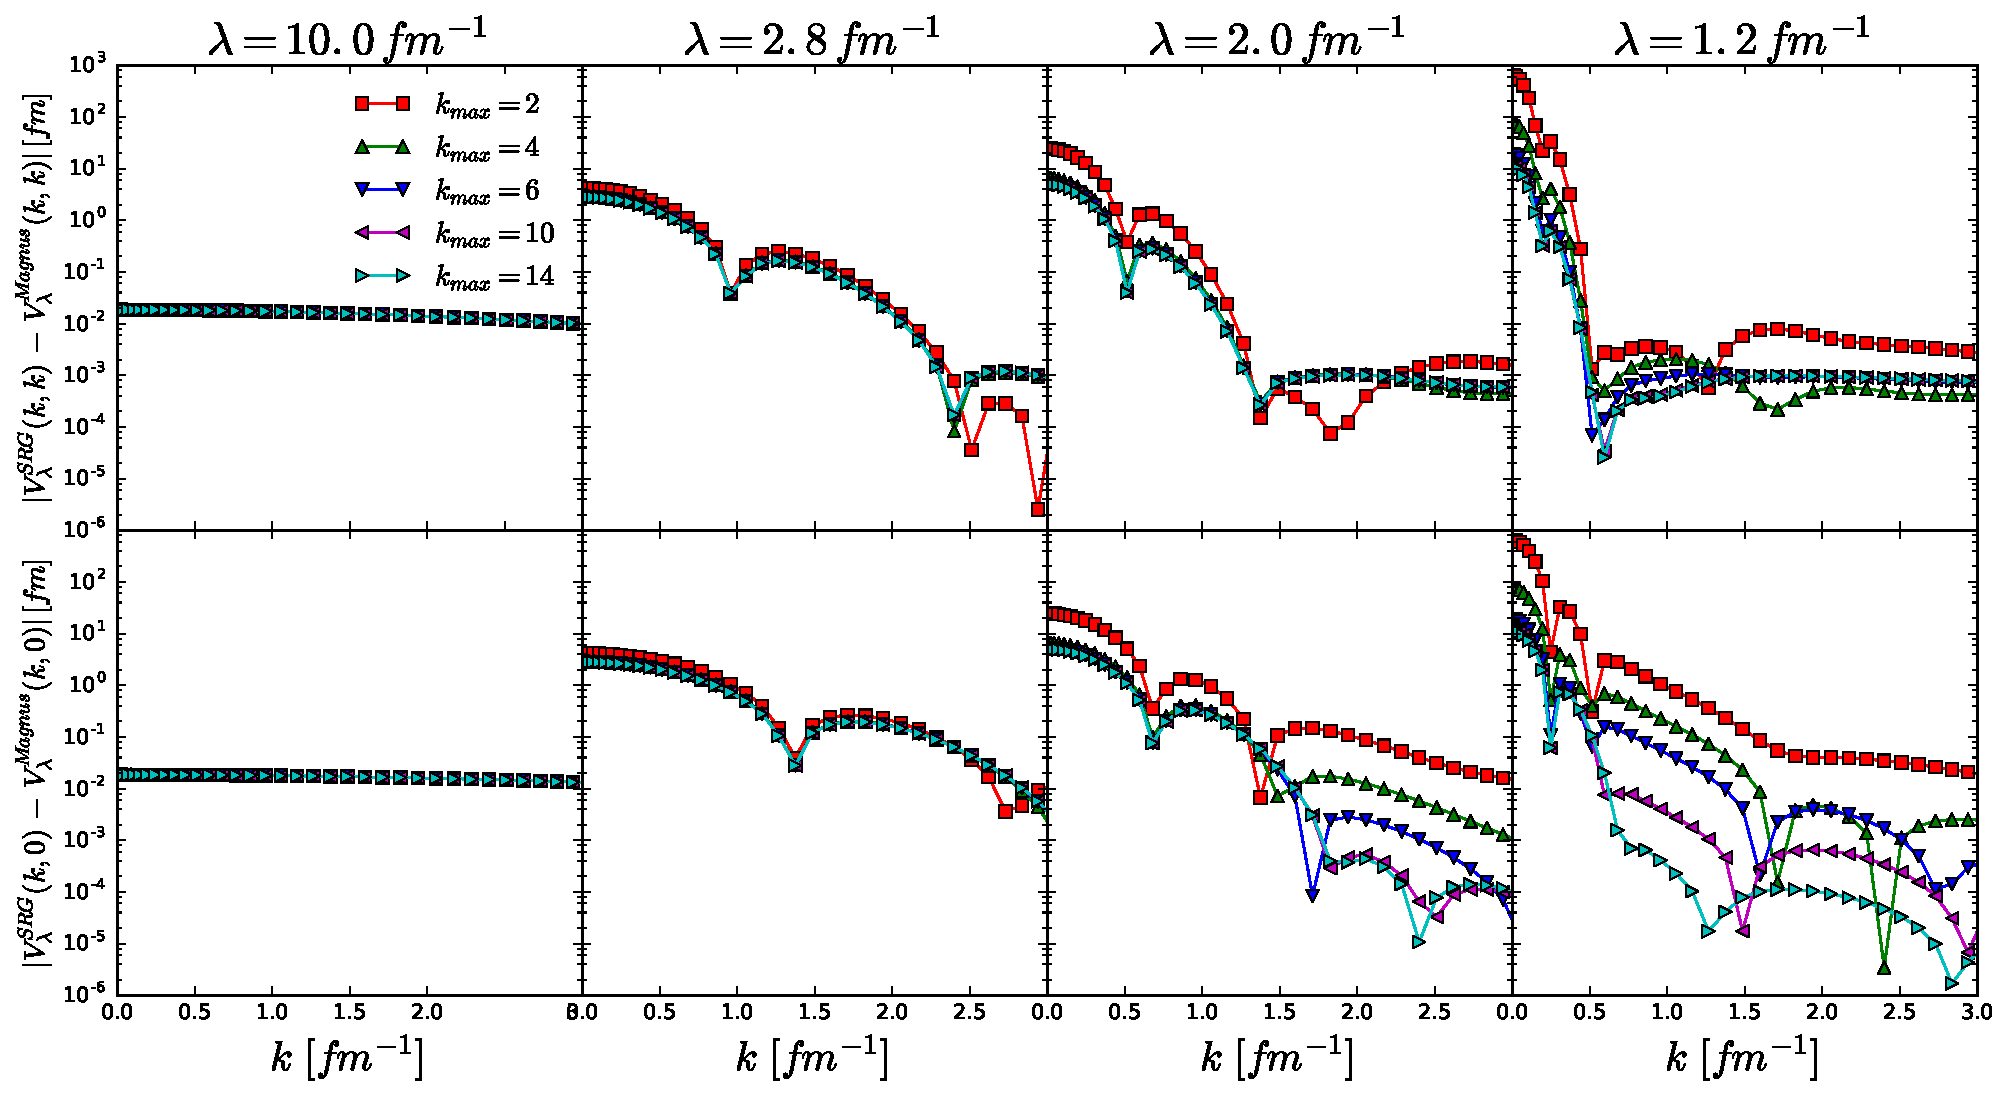
\includegraphics[width=15cm]{mag_diff_Wendt_9_Wilson}
   \hspace*{0.05\textwidth}%
  \caption{Difference in the diagonal and off-diagonal matrix elements of evolved $V_{\lambda}(k,k')$ with $G=H_D$ and $\Lambda=9.0 \, fm^{-1}$ for several values of $\lambda$ and $k_{max}$.}
  \label{fig:mag_diff_Wendt_9_Wilson}
\end{figure}
%
\begin{figure}[H]
  \centering
  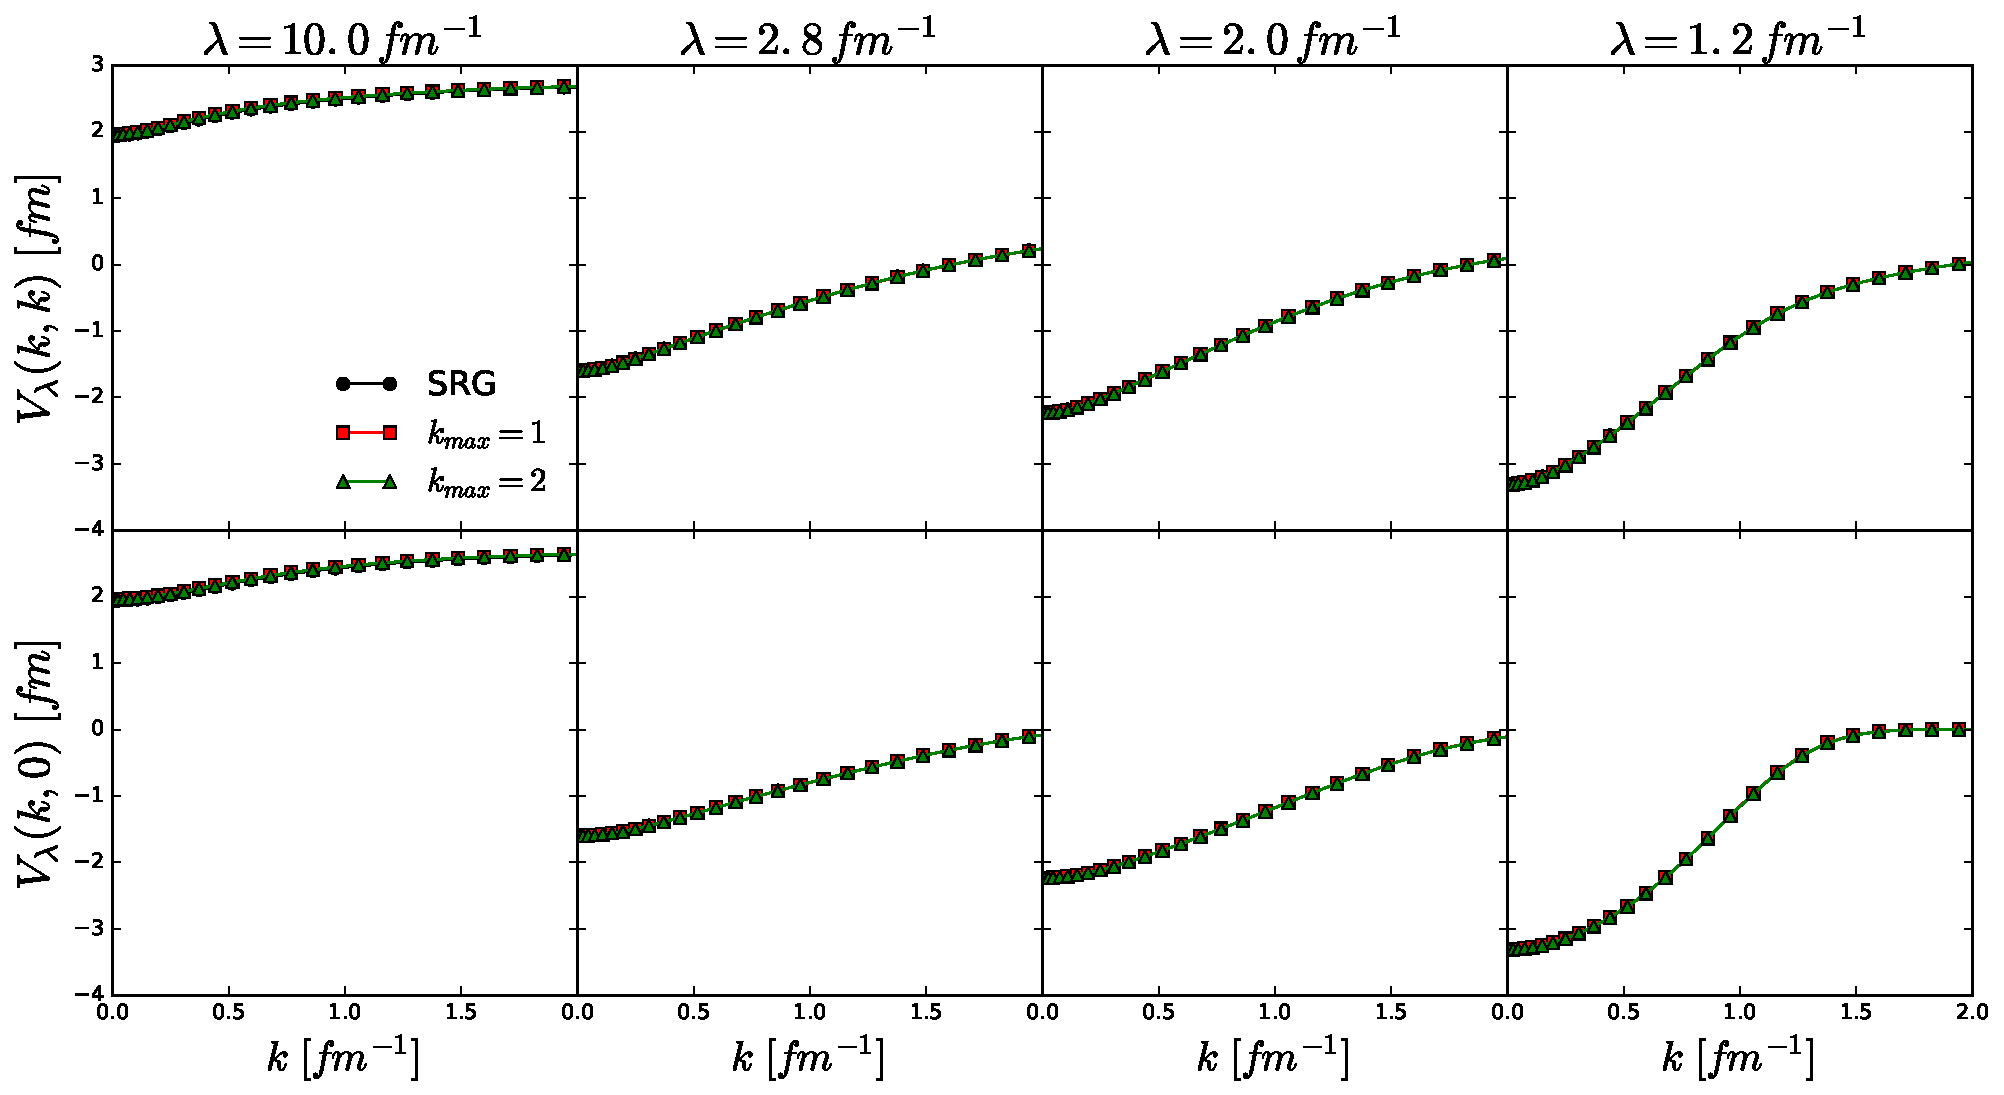
\includegraphics[width=15cm]{mag_diags_offdiags_Wendt_4_Wegner}
   \hspace*{0.05\textwidth}%
  \caption{Diagonal and off-diagonal matrix elements of evolved $V_{\lambda}(k,k')$ with $G=H_{D}$ and $\Lambda=4.0 \, fm^{-1}$ for several values of $\lambda$ and $k_{max}$ compared to the SRG result.}
  \label{fig:mag_diags_offdiags_Wendt_4_Wegner}
\end{figure}
%
In Figures \ref{fig:mag_diff_Wendt_9_Wegner} and \ref{fig:mag_diff_Wendt_9_Wilson} we show the difference in the diagonal and off-diagonal matrix elements between the typical SRG evolved potential and the Magnus evolved potential. The only significant disagreement in evolution comes with the low truncation $k_{max}=2$. Taking the next term ($k_{max}=4$ since the $k=3$ term is zero from $B_3=0$) increases the agreement substantially. Finally, we check the comparison between the typical SRG approach and the Magnus implementation at the lower cutoff of $\Lambda=4.0 \, fm^{-1}$ in Figures \ref{fig:mag_diags_offdiags_Wendt_4_Wegner} and \ref{fig:mag_diags_offdiags_Wendt_4_Wilson}. At the lower cutoff, the agreement is better for even lower truncations in the Magnus series. We see consistent evolution keeping only the first couple terms in the Magnus series.
%
\begin{figure}[H]
  \centering
  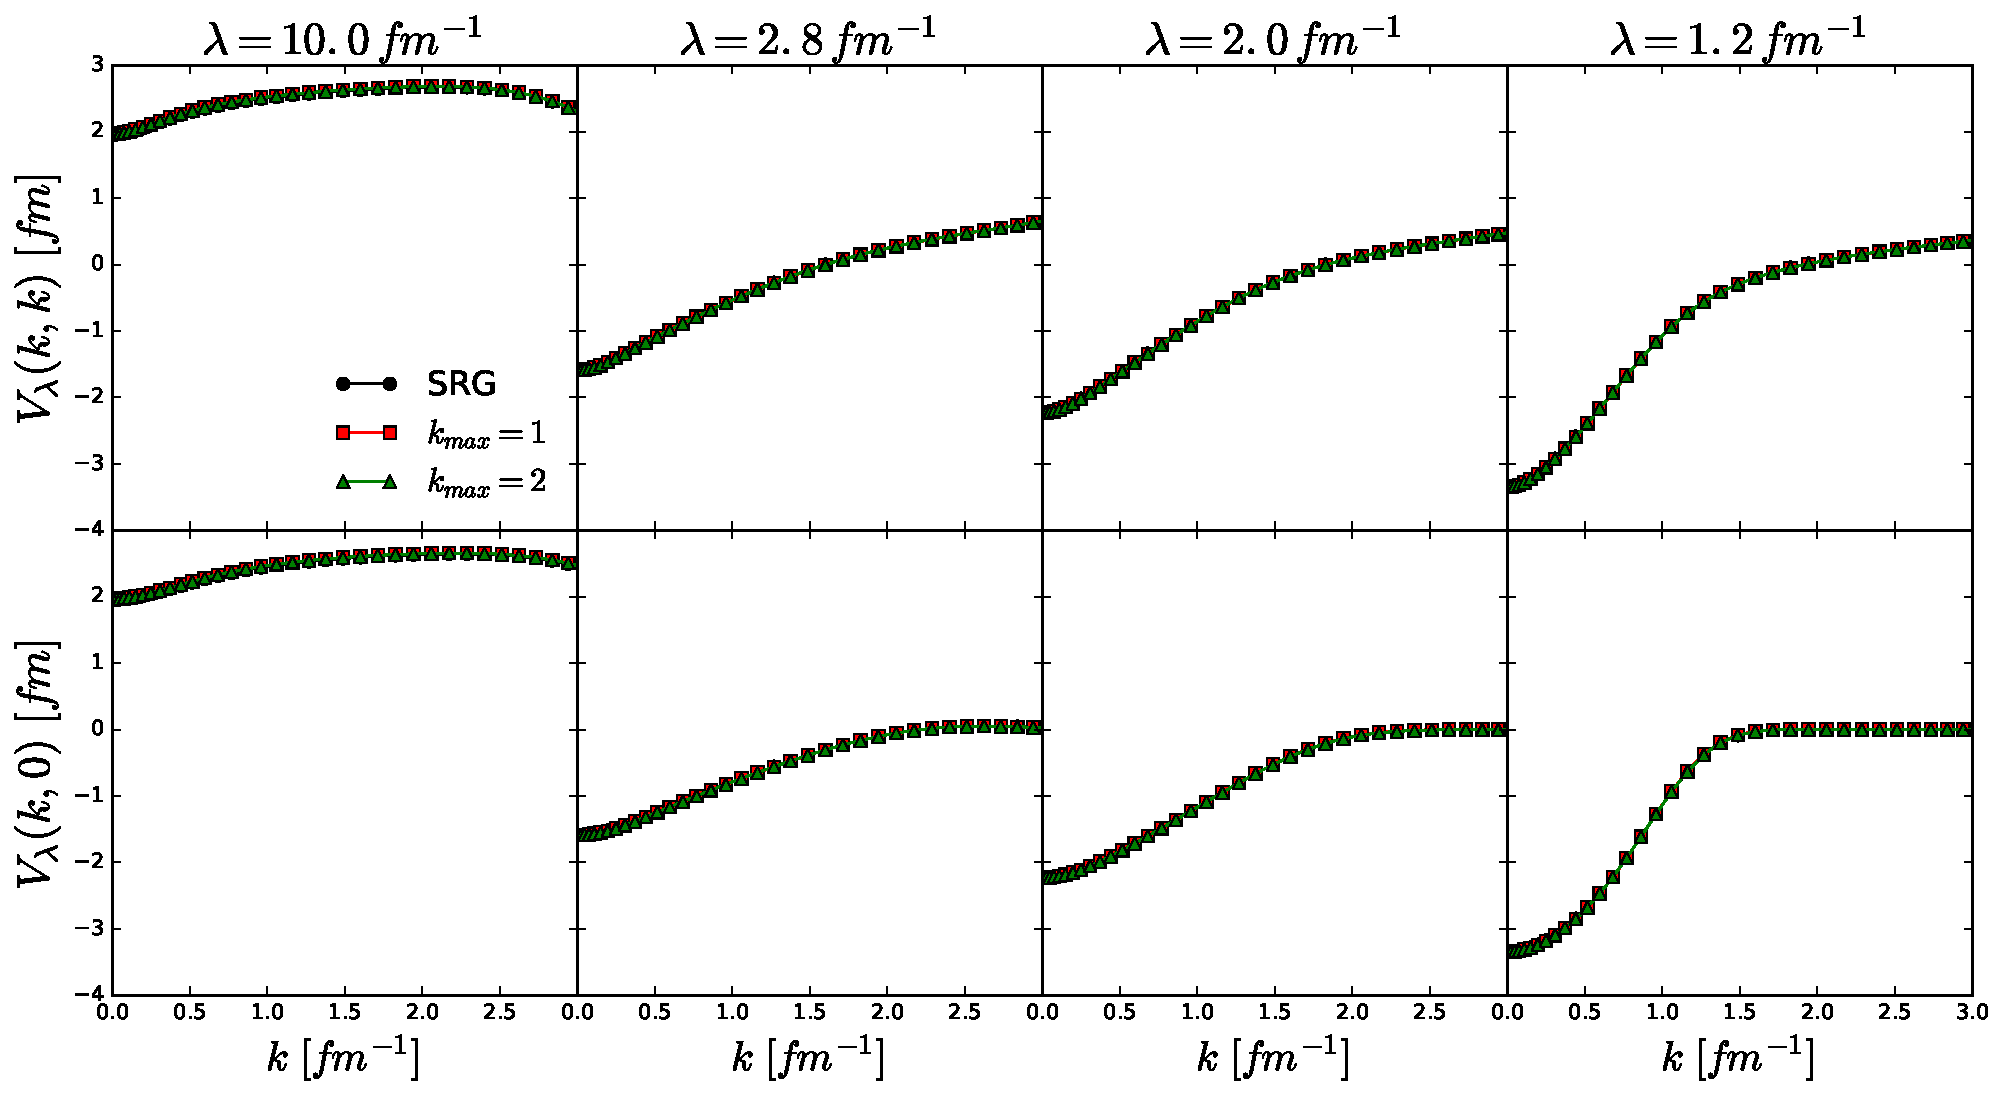
\includegraphics[width=15cm]{mag_diags_offdiags_Wendt_4_Wilson}
   \hspace*{0.05\textwidth}%
  \caption{Diagonal and off-diagonal matrix elements of evolved $V_{\lambda}(k,k')$ with $G=T_{rel}$ and $\Lambda=4.0 \, fm^{-1}$ for several values of $\lambda$ and $k_{max}$ compared to the SRG result.}
  \label{fig:mag_diags_offdiags_Wendt_4_Wilson}
\end{figure}

% .....................................................................................................................................................................................................................................
\subsection{Accuracy of observables}

The Magnus expansion guarantees a unitary transformation in evolving an operator. Thus, the evolved observables are consistent with the initial observables. Here we show some numerical results to illustrate this. In Table \ref{tab:errors} we show values for the relative error in the deuteron bound state energy and the root mean square error (RMSE) in the eigenvalues from the initial and evolved Hamiltonian. With the SRG approach, one cannot avoid compiling ODE solver error in solving the flow equations. The Magnus implementation avoids this issue; this is seen by comparing the orders of magnitude in the Table \ref{tab:errors}. We see about a $10^7$ order of magnitude difference in the relative error of $\epsilon_d$ and a $10^5$ order of magnitude difference in the RMSE going from the SRG approach to the Magnus approach.
%
\begin{table}[H]
\caption{Relative error in the deuteron bound state energy and the root mean square error in eigenvalues where $\tilde{\epsilon}$ denotes an evolved eigenvalue with SRG and Magnus evolved Hamiltonians for $\Lambda=9.0 \, fm^{-1}$ and $\lambda=1.2 \, fm^{-1}$.}
\label{tab:errors}
\begin{ruledtabular}
\begin{tabular}{{>{\centering\arraybackslash}m{1.5in}>{\centering\arraybackslash}m{1in}>{\centering\arraybackslash}m{1.5in}>{\centering\arraybackslash}m{2in}}}
  $  $ & $G$ & $ |\frac{\epsilon_d-\tilde{\epsilon}_d}{\epsilon_d}| $ & $\sqrt{\frac{1}{N} \, \sum_{i}^{N} (\tilde{\epsilon}_i-\epsilon_i)^2}$   [MeV] \\
  \colrule
  SRG & $ $ & $\num{2.428e-06}$ & $\num{2.856e-04}$ \\
  Magnus, $k_{max}=2$ & $H_D$ & $\num{1.040e-12}$ & $\num{6.881e-09}$ \\
  Magnus, $k_{max}=14$ & $ $ & $\num{5.727e-13}$ & $\num{6.903e-09}$ \\ \hline
  SRG & $ $ & $\num{1.325e-04}$ & $\num{1.596e-04}$ \\
  Magnus, $k_{max}=2$ & $T_{rel}$ & $\num{1.542e-11}$ & $\num{6.770e-09}$ \\
  Magnus, $k_{max}=14$ & $ $ & $\num{3.418e-12}$ & $\num{6.674e-09}$ \\
\end{tabular}
\end{ruledtabular}
\end{table}
%
In Figure \ref{fig:initial_phase_shifts} we show the phase shifts in the $^{3}S_{1}-^{3}D_{1}$ coupled channel for two cutoffs in $\Lambda$. Phase shifts should also be consistent from the bare to evolved potential from unitarity. In Figure \ref{fig:evolved_phase_shifts_diff} we show the difference in the bare ($\lambda=\infty$) and evolved ($\lambda=1.2$) phase shifts using the typical SRG approach and the Magnus expansion at two truncations. Up to $E_{lab} \sim 100 \, MeV$ the differences are very small for both methods. At higher lab energies, the difference is more sensitive to the truncation in the Magnus series. This is illustrated by the large peak at $E_{lab} \sim 100 \, MeV$ for $k_{max}=2$ and $G=H_D$ in Figure \ref{fig:evolved_phase_shifts_diff}.
%
\begin{figure}[H]
  \centering
  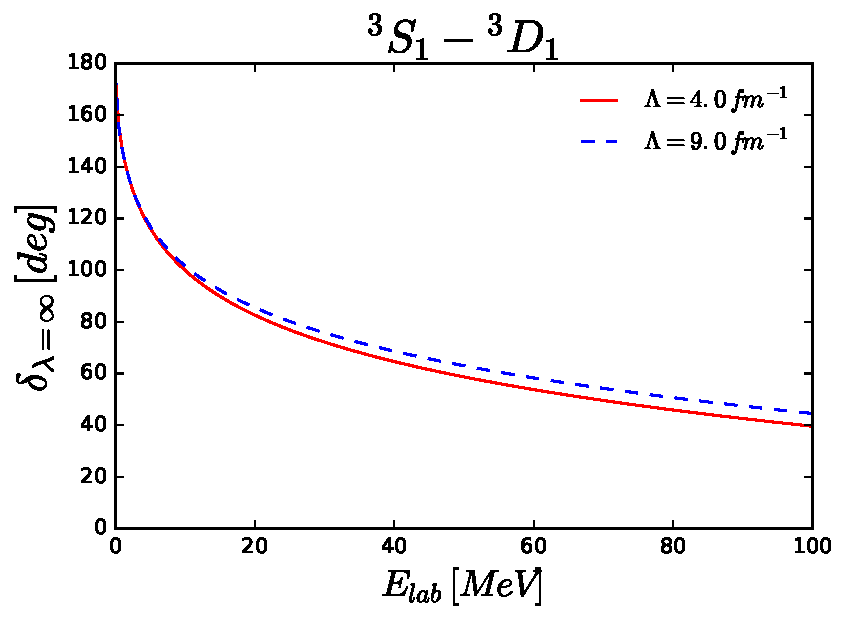
\includegraphics[width=10cm]{initial_phase_shifts}
   \hspace*{0.05\textwidth}%
  \caption{$^{3}S_{1}$ phase shifts for $\Lambda=4.0$ and $9.0 \, fm^{-1}$.}
  \label{fig:initial_phase_shifts}
\end{figure}
%
\begin{figure}[H]
  \centering
  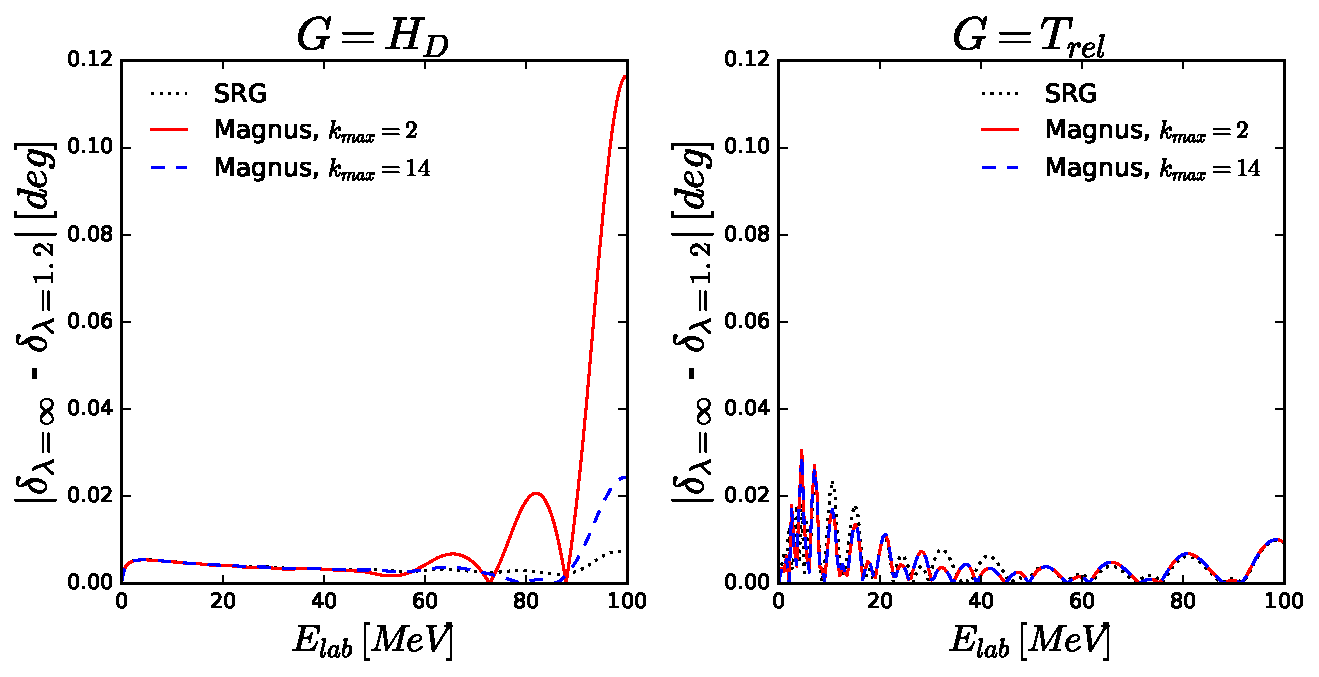
\includegraphics[width=15cm]{evolved_phase_shifts_diff}
   \hspace*{0.05\textwidth}%
  \caption{Difference in the $^{3}S_{1}$ phase shifts with $\Lambda=9.0 \, fm^{-1}$ for SRG and Magnus evolved potentials.}
  \label{fig:evolved_phase_shifts_diff}
\end{figure}

% .....................................................................................................................................................................................................................................
\subsection{RKE semi-local potentials}

The previous results used a non-local potential where both the one-pion exchange potential and contact force are regulated with Eq. (\ref{eq:non_local_reg}). One might ask how high cutoffs affect the SRG procedure for potentials that are regulated differently. This is an interesting problem in its own right, and we leave a complete analysis of this as a further study. Here we sample this problem by showing SRG and Magnus results with a semi-local LO NN potential \cite{Reinert:2018} where the regulators have the following form:
%
\begin{subequations}
\label{eq:semi_local_regulator}
\begin{eqnarray}
f_{1\pi}(q) = e^{-(q^2+M_{\pi}^2)/\Lambda^2},
\label{eq:opep_regulator} \\
%
f_{cont}(k',k) = e^{-(k^2+k'^2)/\Lambda^2},
\label{eq:contact_regulator}
\end{eqnarray}
\end{subequations}
%
where $q=|\vec{k}'-\vec{k}|$. The first function regulates the OPEP locally while the second regulates the contact force non-locally. \\

Notice that the cutoff is not consistent numerically between the two cases in the sense that functional form of the regulator controls the strength of the cutoff (i.e., $\Lambda=4.0 \, fm^{-1}$ for the non-local potential is not the same as $\Lambda=4.0 \, fm^{-1}$ for the semi-local potential). This is seen in Table \ref{tab:RKE_bound_states} by noting the presence of a spurious, deeply bound state at $\Lambda=4.0 \, fm^{-1}$. This was not the case with the non-local potential. Higher values of $\Lambda$ correspond to a stronger cutoff for the semi-local potential compared to the non-local potential. Thus, we only need to take $\Lambda \approx 4.0 \, fm^{-1}$ to produce a potential with a spurious bound state.
%
\begin{table}[H]
\caption{Bound state values for deuteron, $\epsilon_d$, and the spurious, deeply bound state, $\epsilon_s$ in units MeV for two cutoffs in $\Lambda$}
\label{tab:RKE_bound_states}
\begin{ruledtabular}
\begin{tabular}{{>{\centering\arraybackslash}m{2in} >{\centering\arraybackslash}m{2in}>{\centering\arraybackslash}m{2in}}}
  $\Lambda \,\,\, [fm^{-1}]$ & $\epsilon_d$  [MeV] & $\epsilon_s$  [MeV] \\
  \colrule
  $3.0$ & $-2.224$ & - \\
  $4.0$ & $-2.225$ & $-1311.442$ \\
\end{tabular}
\end{ruledtabular}
\end{table}
%
\begin{figure}[H]
  \centering
  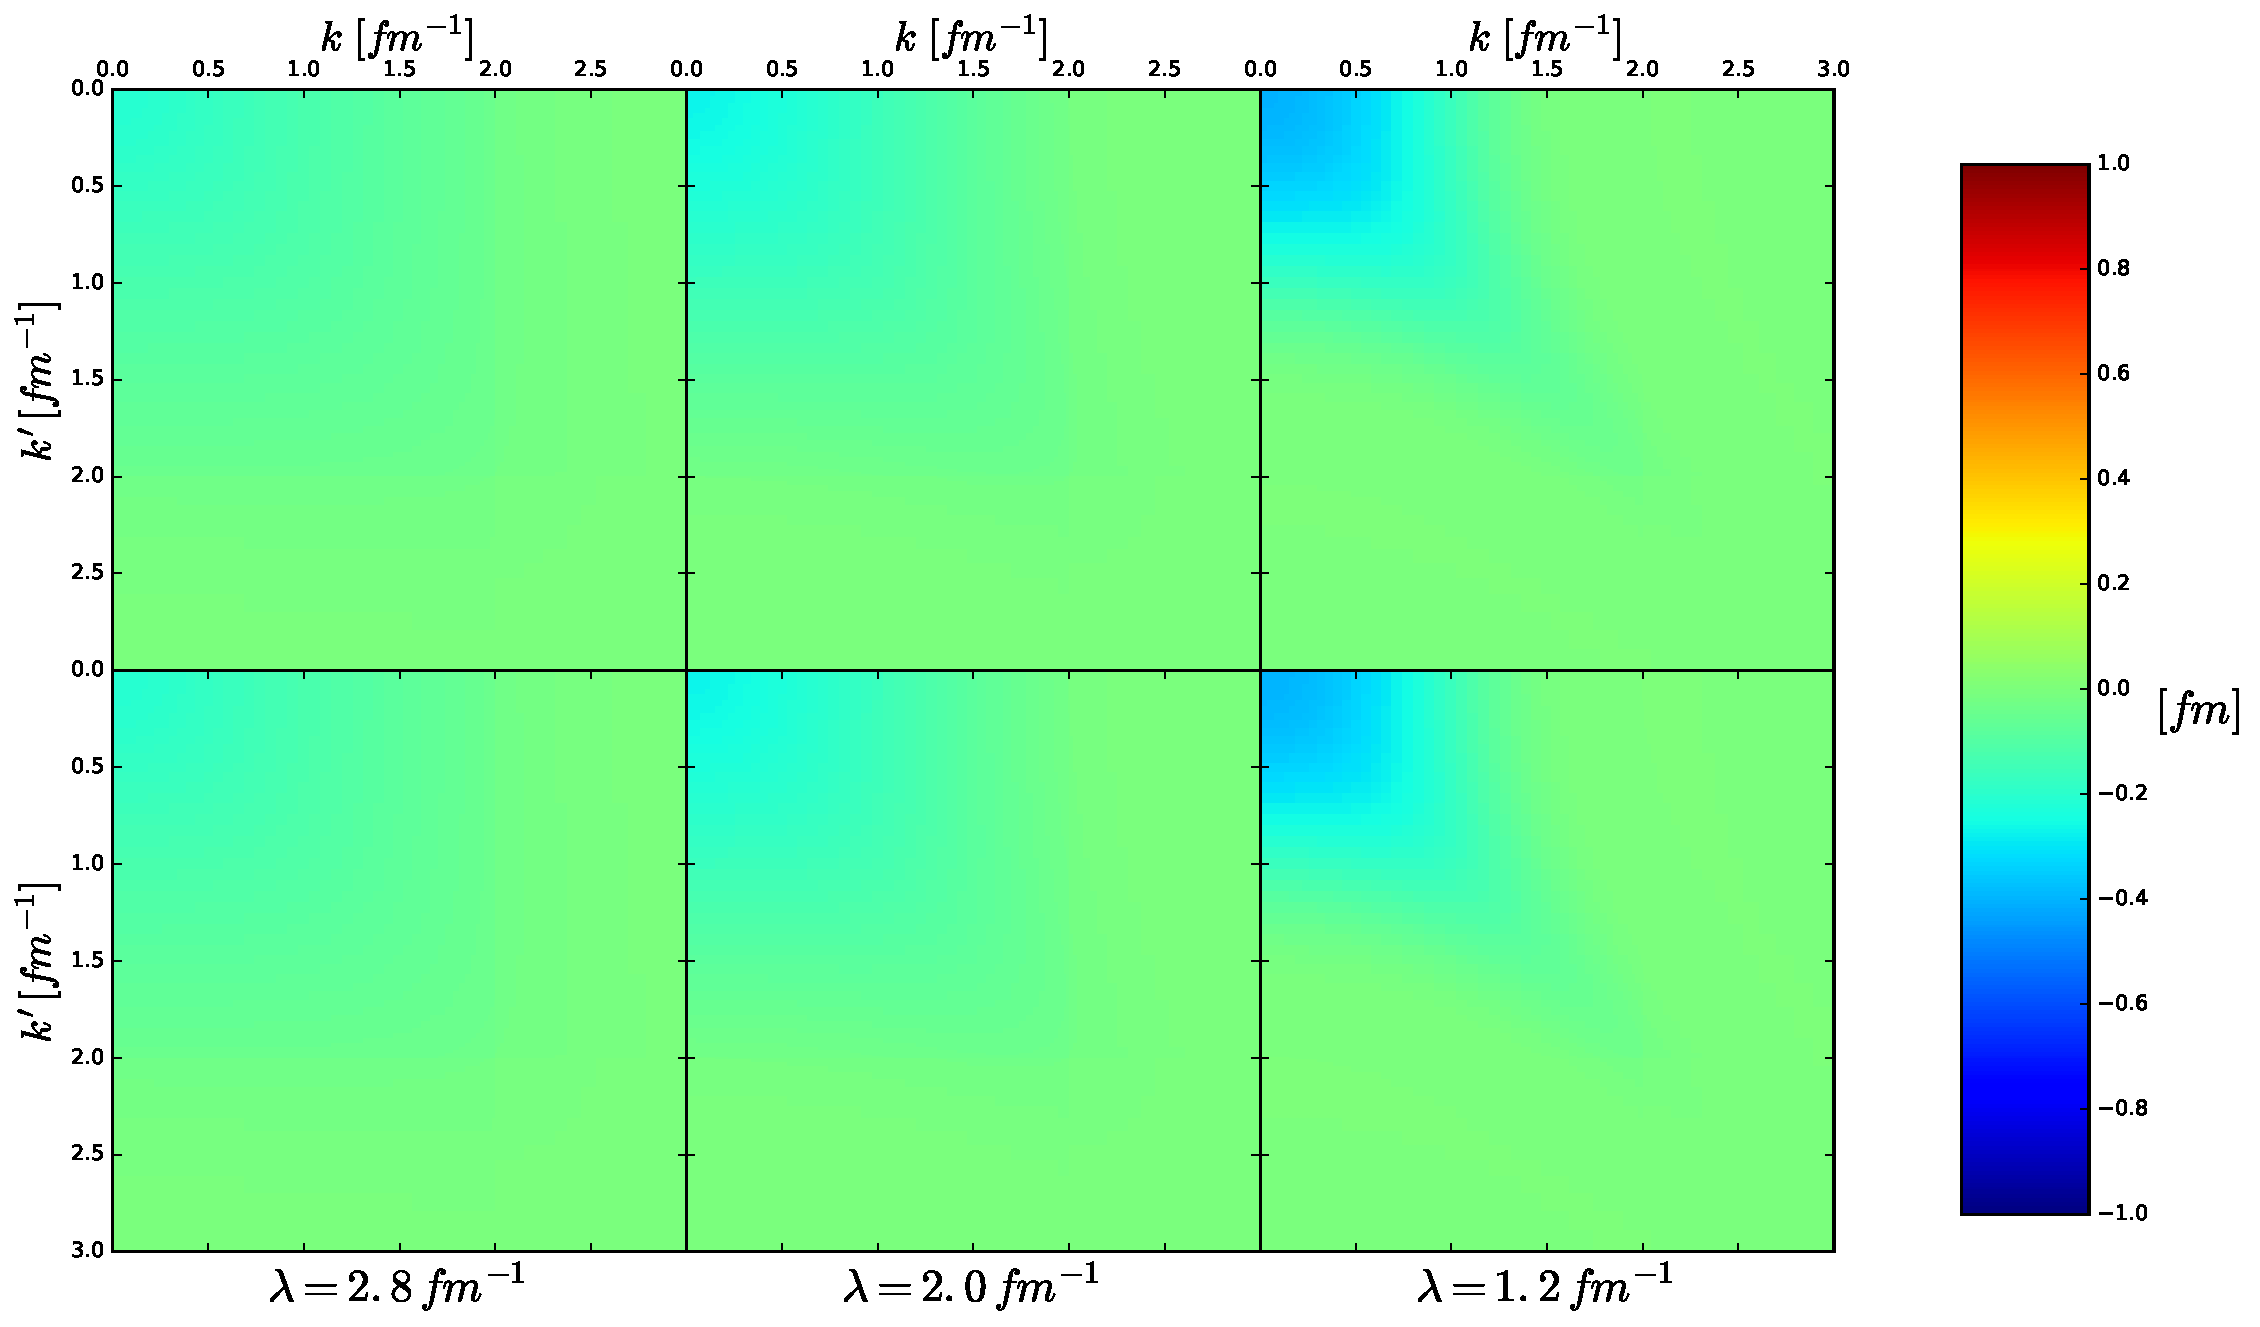
\includegraphics[width=14cm]{srg_contours_RKE_3}
   \hspace*{0.05\textwidth}%
  \caption{Contour of SRG evolved $V_{\lambda}(k,k')$ with $\Lambda=3.0\,fm^{-1}$, $G=T_{rel}$ (top) and $G=H_{D}$ (bottom) for several values of $\lambda$.}
  \label{fig:srg_contours_RKE_3}
\end{figure}
%
Figures \ref{fig:srg_contours_RKE_3} and \ref{fig:srg_contours_RKE_4} show the SRG evolution of the semi-local potential. These figures reinforce the result from before, namely that the evolution is generator dependent at high cutoffs. In Figure \ref{fig:srg_contours_RKE_3} where $\Lambda=3.0 \, fm^{-1}$, we see that the choice in SRG generator is not so important as before (the analogous non-local figure is Figure \ref{fig:srg_contours_Wendt_4}). Again, both generators decouple the potential in similar fashion. But at the higher cutoff of $\Lambda=4.0 \, fm^{-1}$ where the spurious, deeply bound state is present, the $G=T_{rel}$ and $G=H_D$ differ in the same manner as with the non-local potential. The Wegner generator safely decouples the spurious bound state from the low-momentum part of the potential whereas the $G=T_{rel}$ choice keeps the spurious bound state at low-momentum. This generator behavior is independent of how the potential is regulated. One deviation from the non-local case is that the Wegner generator decouples the spurious bound state at a lower value of momentum, $k \approx 1.1 \, fm^{-1}$, compared to $k \approx 1.75 \, fm^{-1}$ for the non-local case. It is not clear what leads to where the spurious bound state is decoupled. It is also not fully understood how to compare cutoff values for potentials that are regulated differently. These questions are left as future work.
%
\begin{figure}[H]
  \centering
  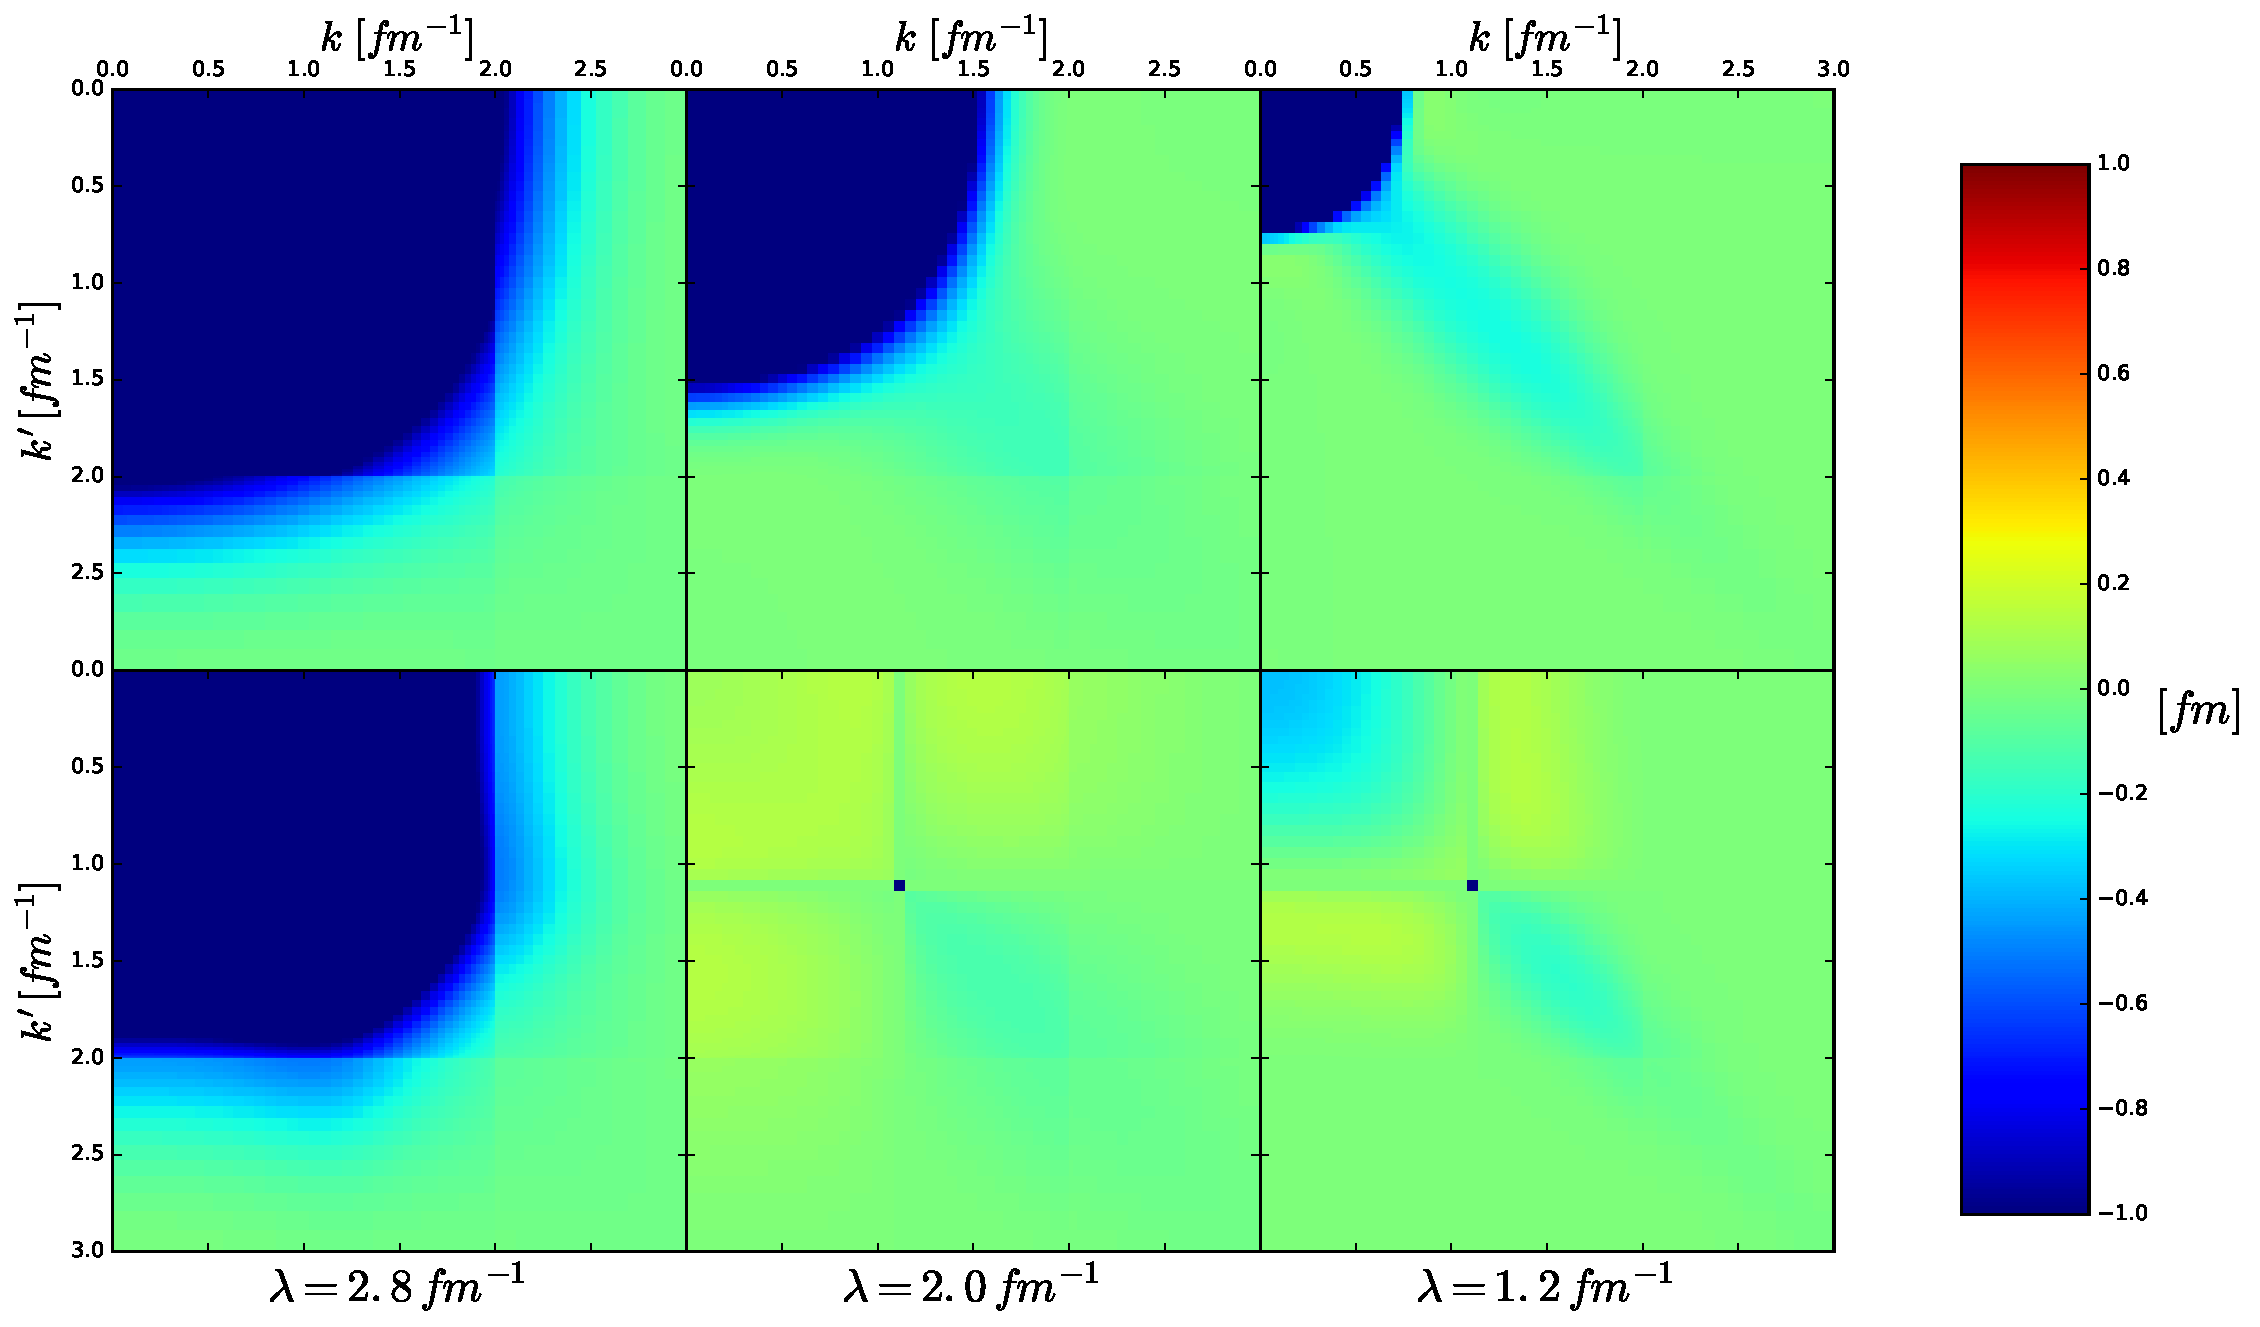
\includegraphics[width=14cm]{srg_contours_RKE_4}
   \hspace*{0.05\textwidth}%
  \caption{Contour of SRG evolved $V_{\lambda}(k,k')$ with $\Lambda=4.0\,fm^{-1}$, $G=T_{rel}$ (top) and $G=H_{D}$ (bottom) for several values of $\lambda$.}
  \label{fig:srg_contours_RKE_4}
\end{figure}
%
Figures \ref{fig:mag_contours_RKE_4_Wegner} and \ref{fig:mag_contours_RKE_4_Wilson} compare Magnus evolved potentials and SRG evolved potentials for $G=H_D$ and $G=T_{rel}$ respectively. The Magnus implementation matches the SRG result at lower truncations than in the non-local case. The agreement is good for $k_{max} \gtrsim 1$ with $k_{max}=0$ being the only exception. This is seen more explicitly in Figures \ref{fig:mag_diags_offdiags_RKE_4_Wegner} and \ref{fig:mag_diags_offdiags_RKE_4_Wilson} which show the diagonal and off-diagonal elements of the evolving potential. The Magnus implementation also matches the Wegner and $T_{rel}$ spurious bound state decoupling behavior as in the non-local case. These results reinforce the idea that the Magnus implementation matches SRG transformations for even the most stringent cases which should inspire confidence for using the Magnus expansion in investigating systems with intruder states in the IMSRG context.
%
\begin{figure}[H]
  \centering
  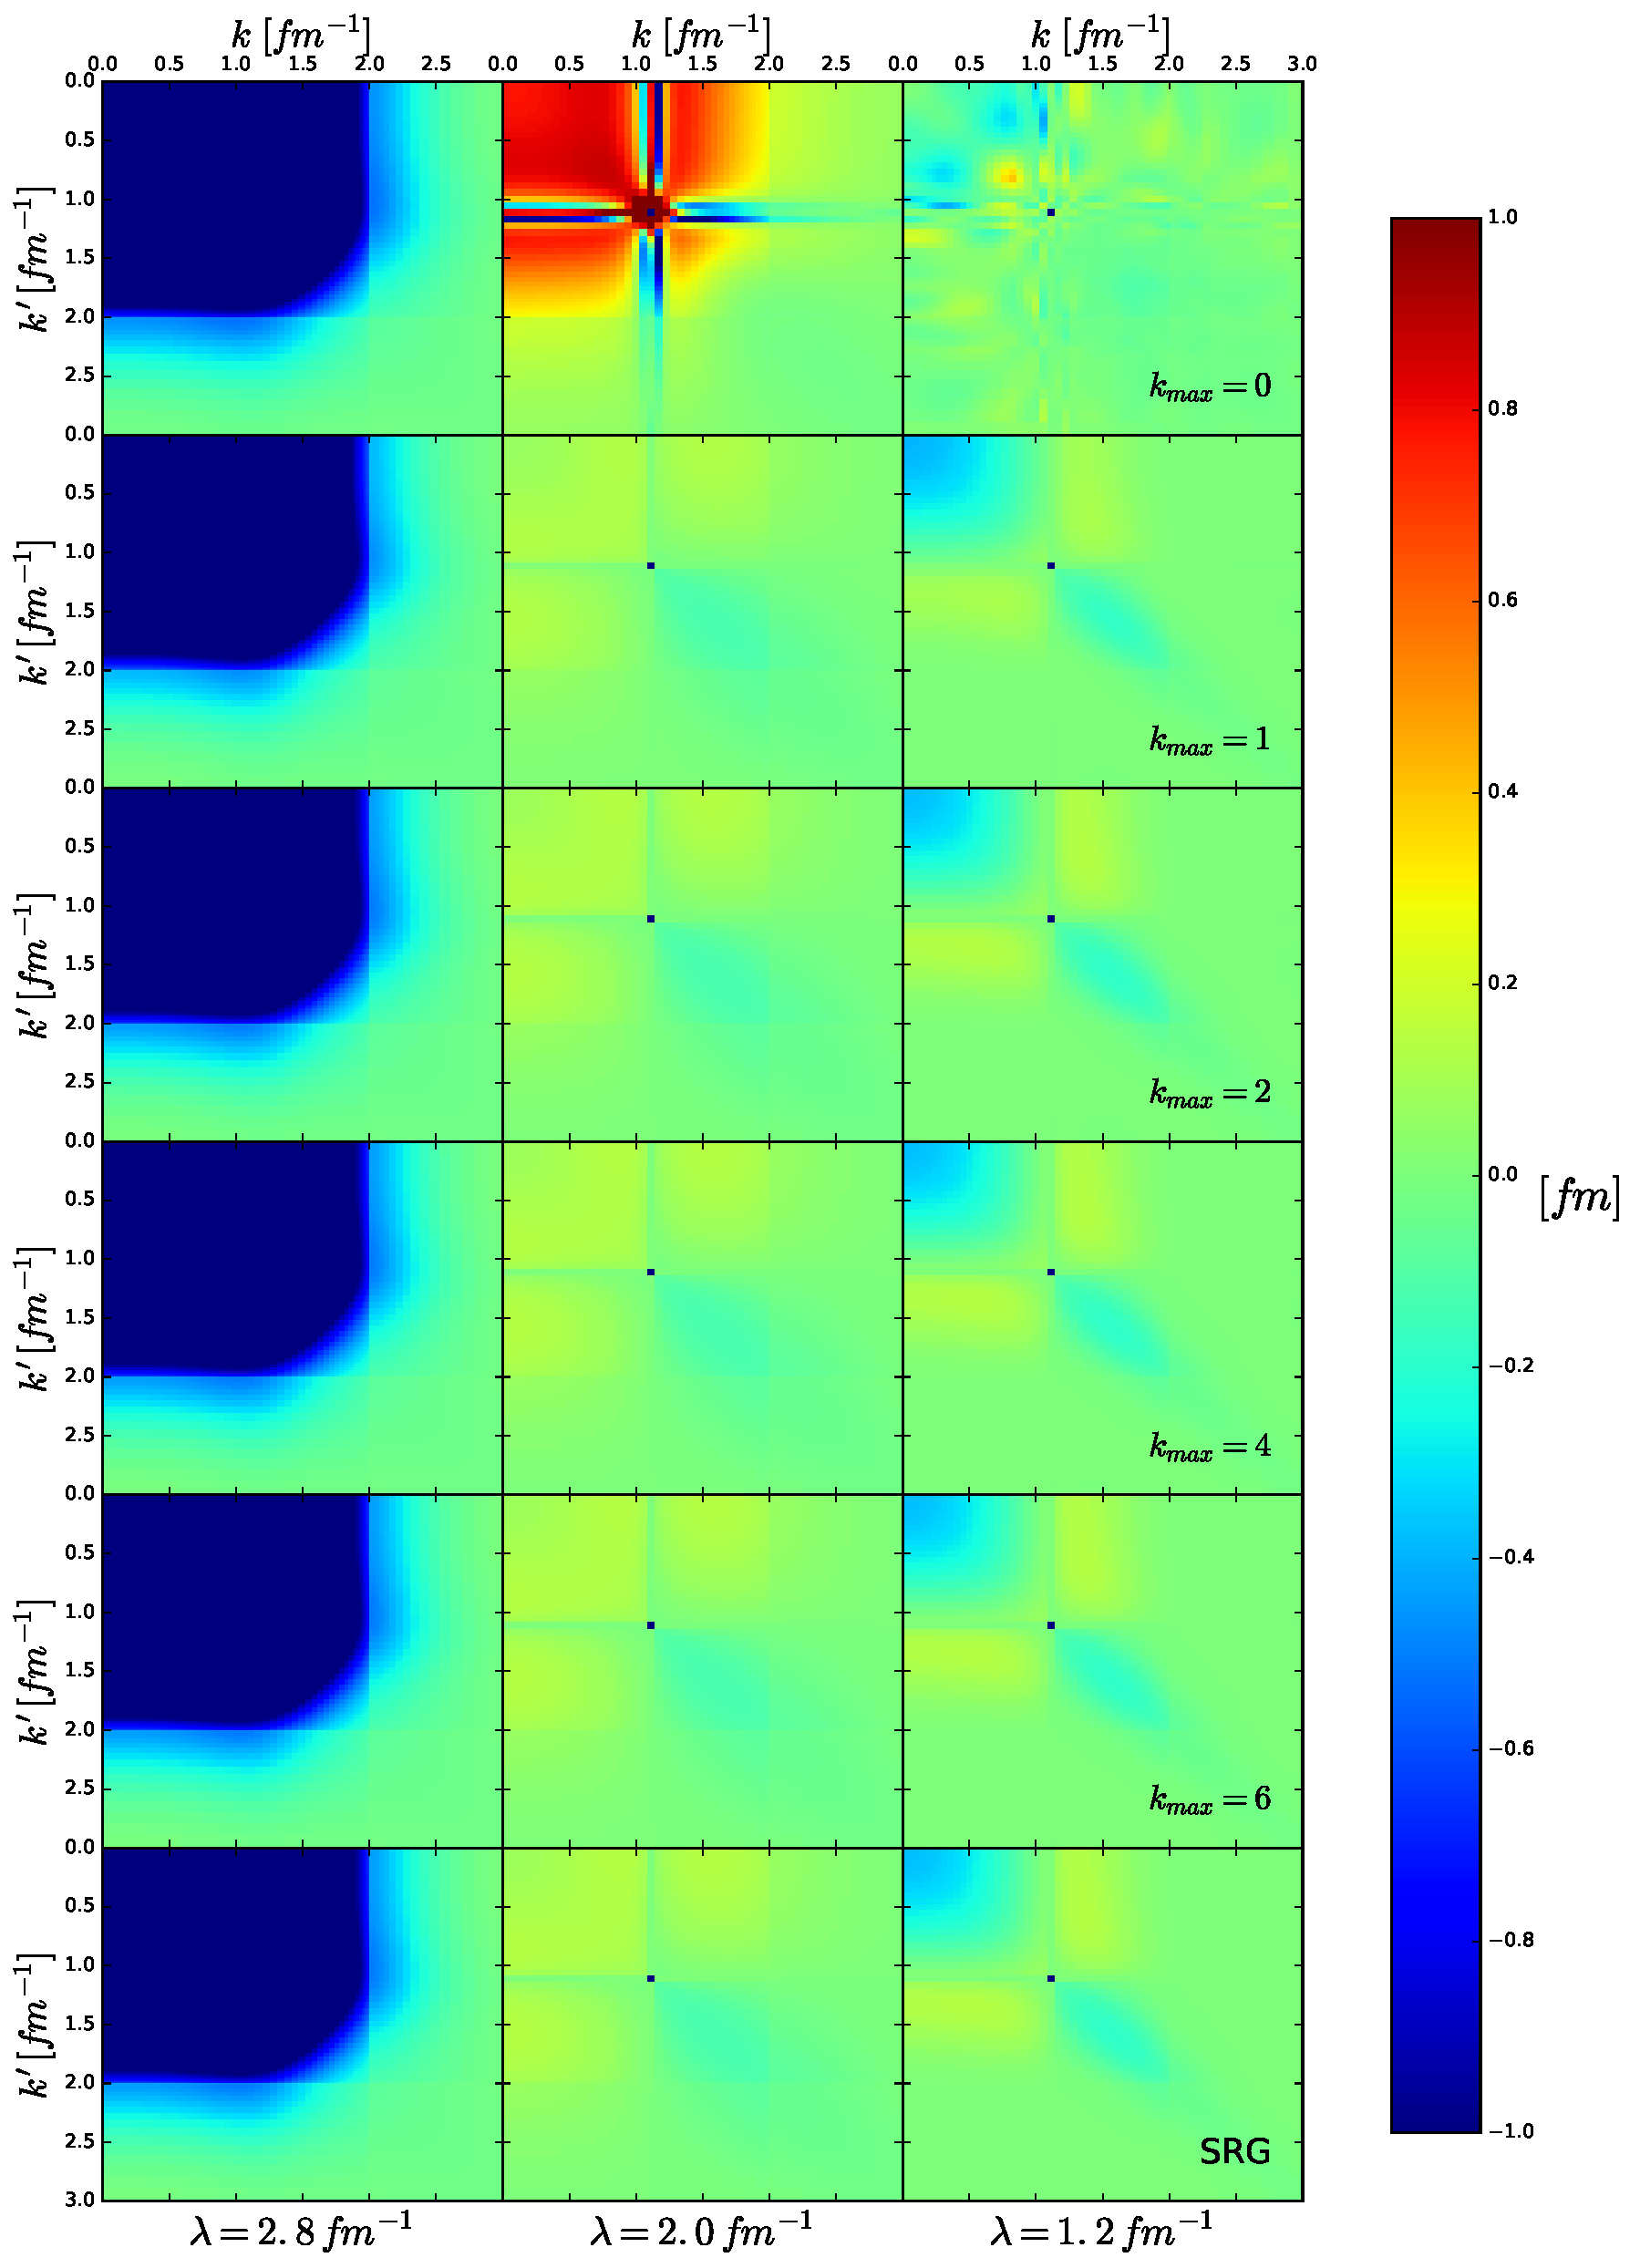
\includegraphics[width=15cm]{mag_contours_RKE_4_Wegner}
   \hspace*{0.05\textwidth}%
  \caption{Contour of evolved $V_{\lambda}(k,k')$ with $\Lambda=4.0\,fm^{-1}$ and $G=H_{D}$ for several values of $\lambda$. Each row corresponds to a different truncation in the Magnus expansion (0, 1, 2, 4, 6) with the last row being the SRG result.}
  \label{fig:mag_contours_RKE_4_Wegner}
\end{figure}
%
\begin{figure}[H]
  \centering
  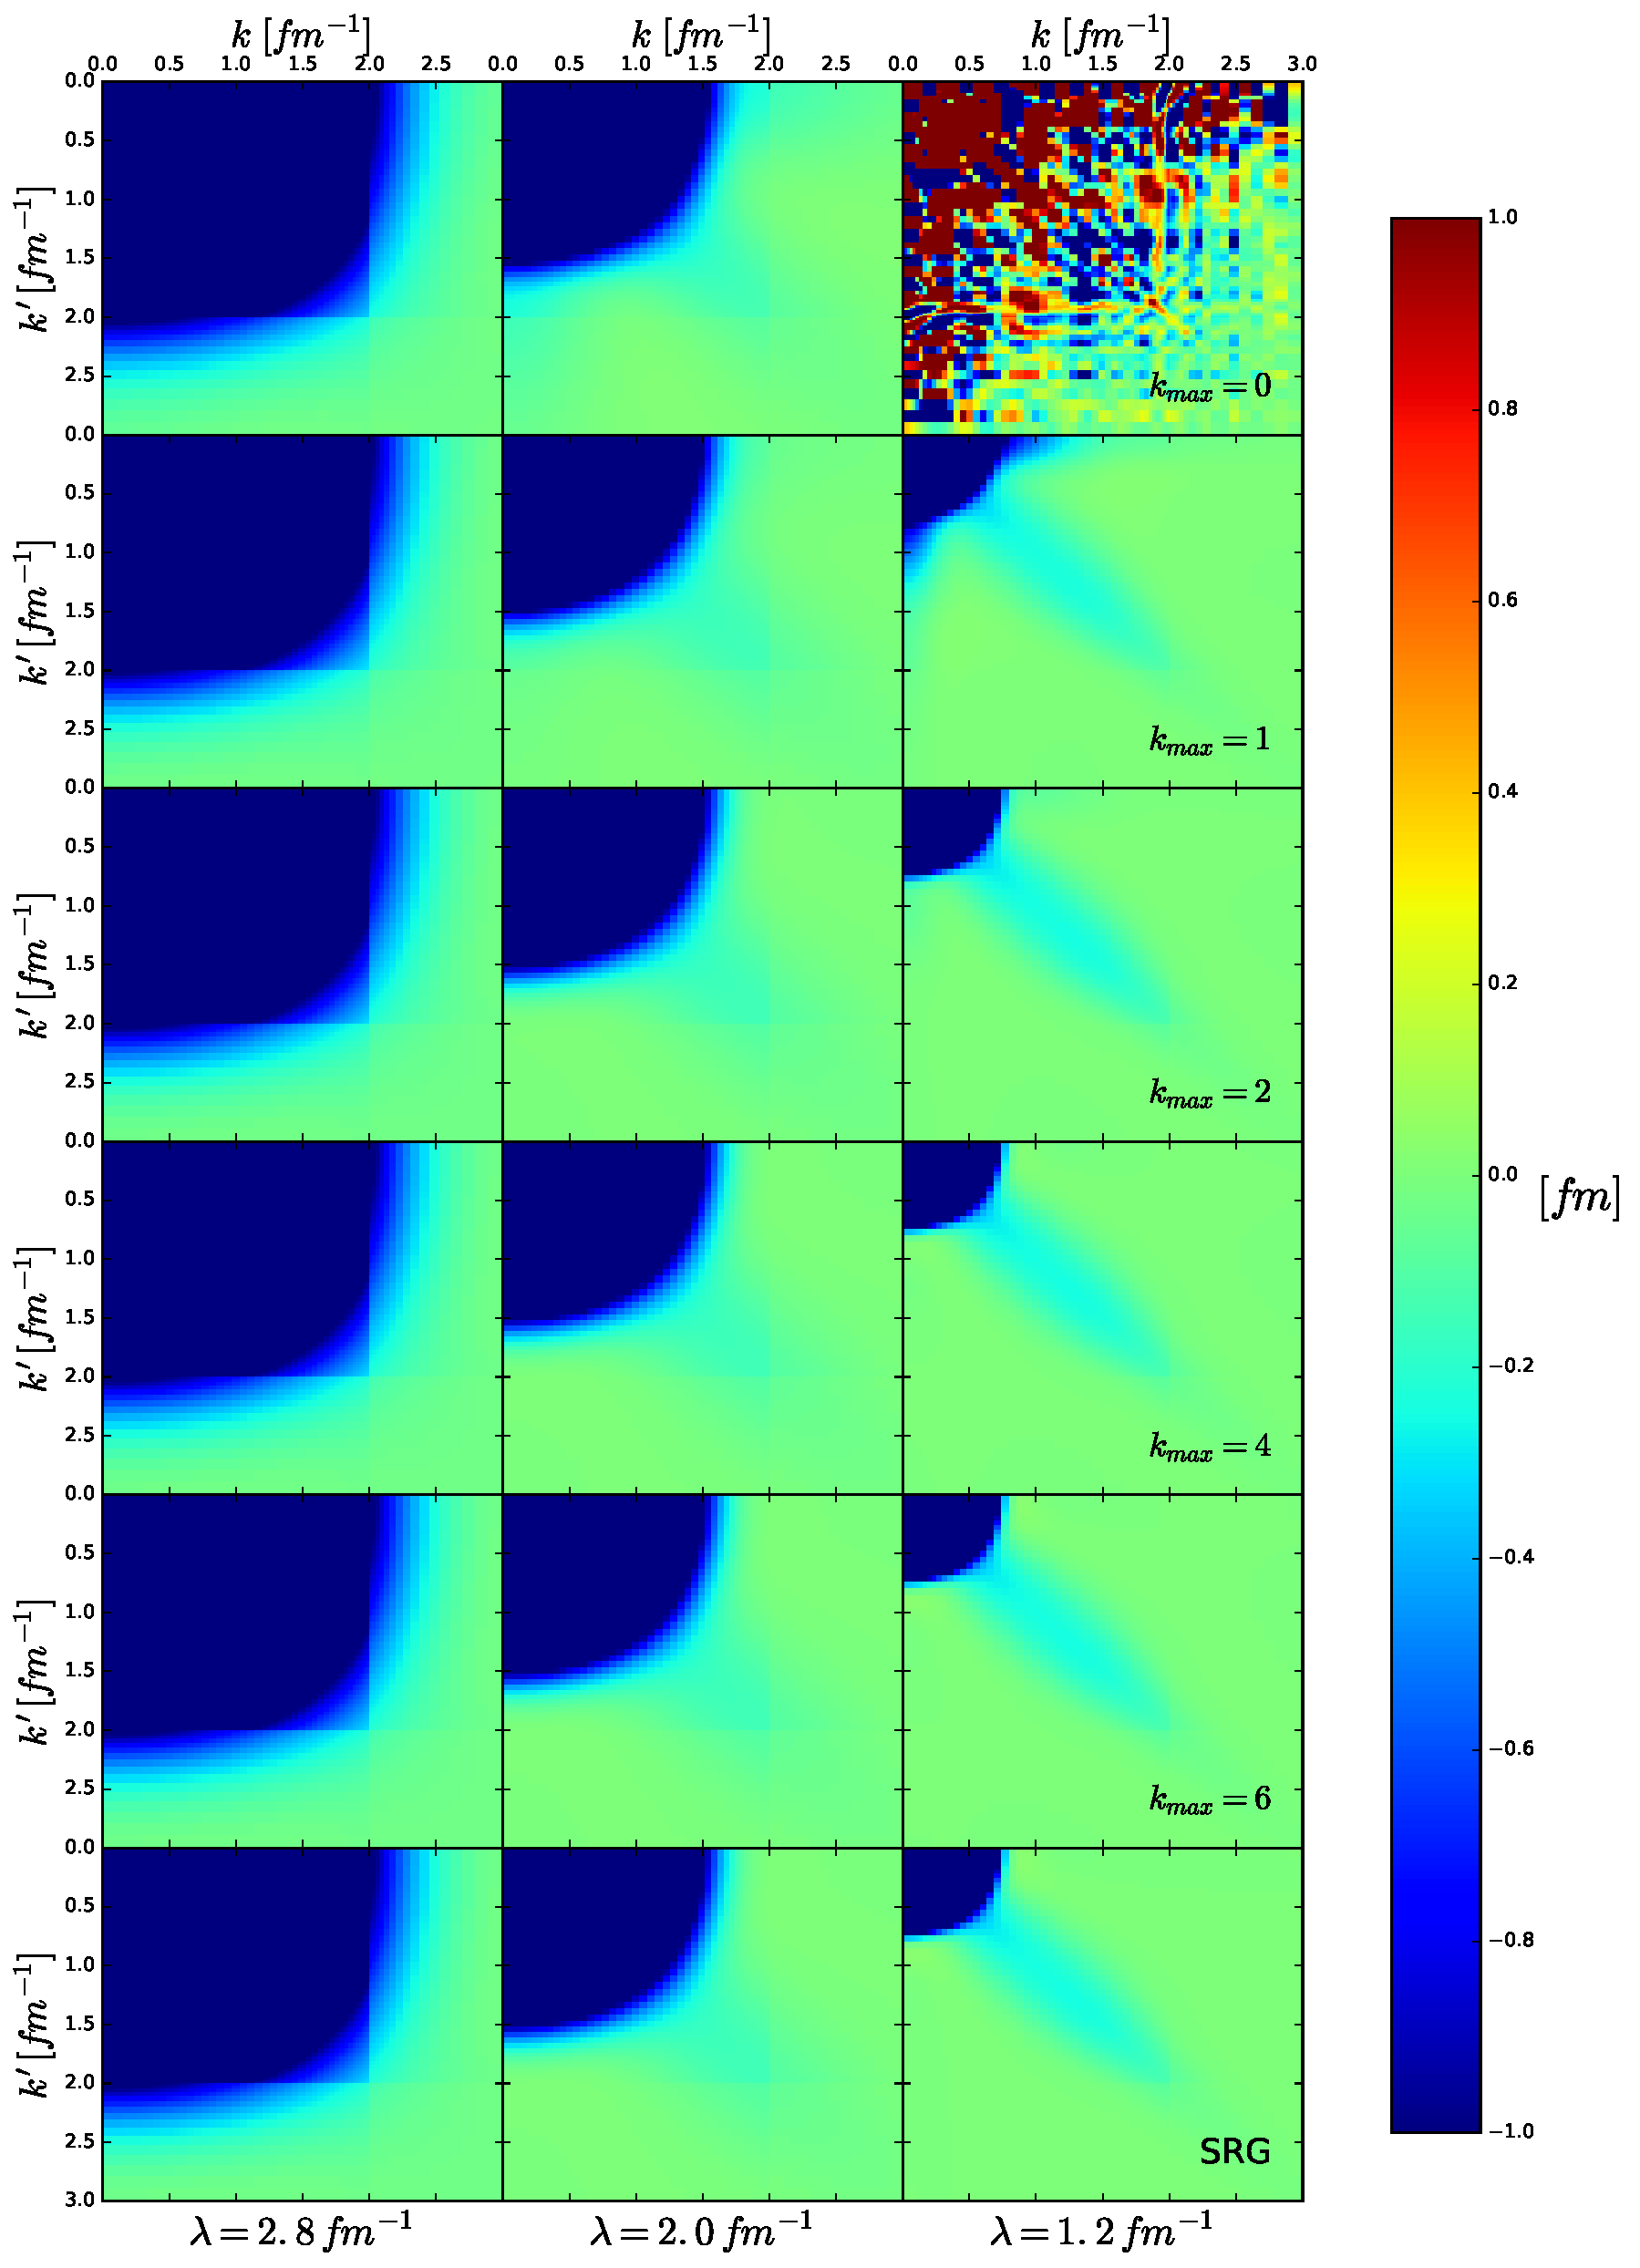
\includegraphics[width=15cm]{mag_contours_RKE_4_Wilson}
   \hspace*{0.05\textwidth}%
  \caption{Contour of evolved $V_{\lambda}(k,k')$ with $\Lambda=4.0\,fm^{-1}$ and $G=T_{rel}$ for several values of $\lambda$. Each row corresponds to a different truncation in the Magnus expansion (0, 1, 2, 4, 6) with the last row being the SRG result.}
  \label{fig:mag_contours_RKE_4_Wilson}
\end{figure}
%
\begin{figure}[H]
  \centering
  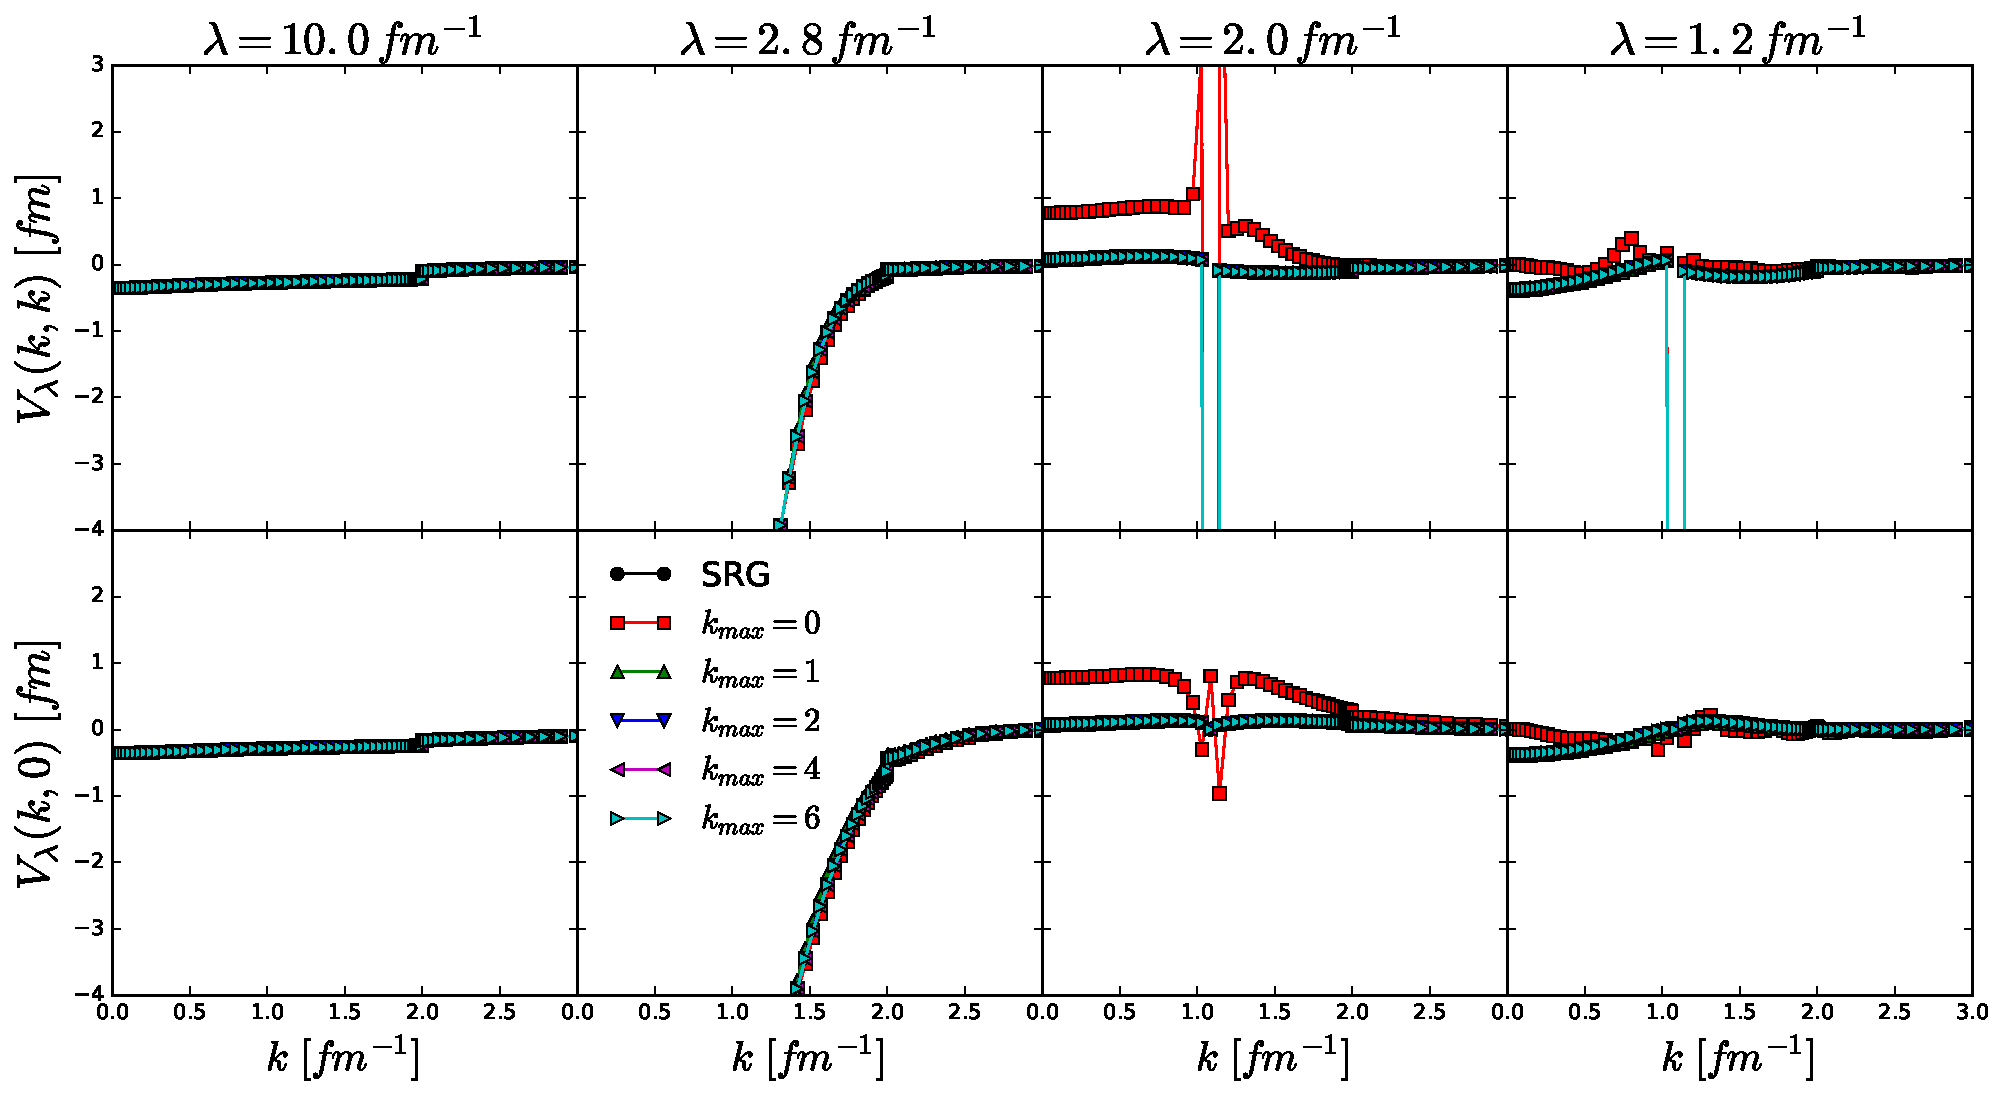
\includegraphics[width=15cm]{mag_diags_offdiags_RKE_4_Wegner}
   \hspace*{0.05\textwidth}%
  \caption{Diagonal and off-diagonal matrix elements of evolved $V_{\lambda}(k,k')$ with $G=H_{D}$ and $\Lambda=4.0 \, fm^{-1}$ for several values of $\lambda$ and $k_{max}$ compared to the SRG result.}
  \label{fig:mag_diags_offdiags_RKE_4_Wegner}
\end{figure}
%
\begin{figure}[H]
  \centering
  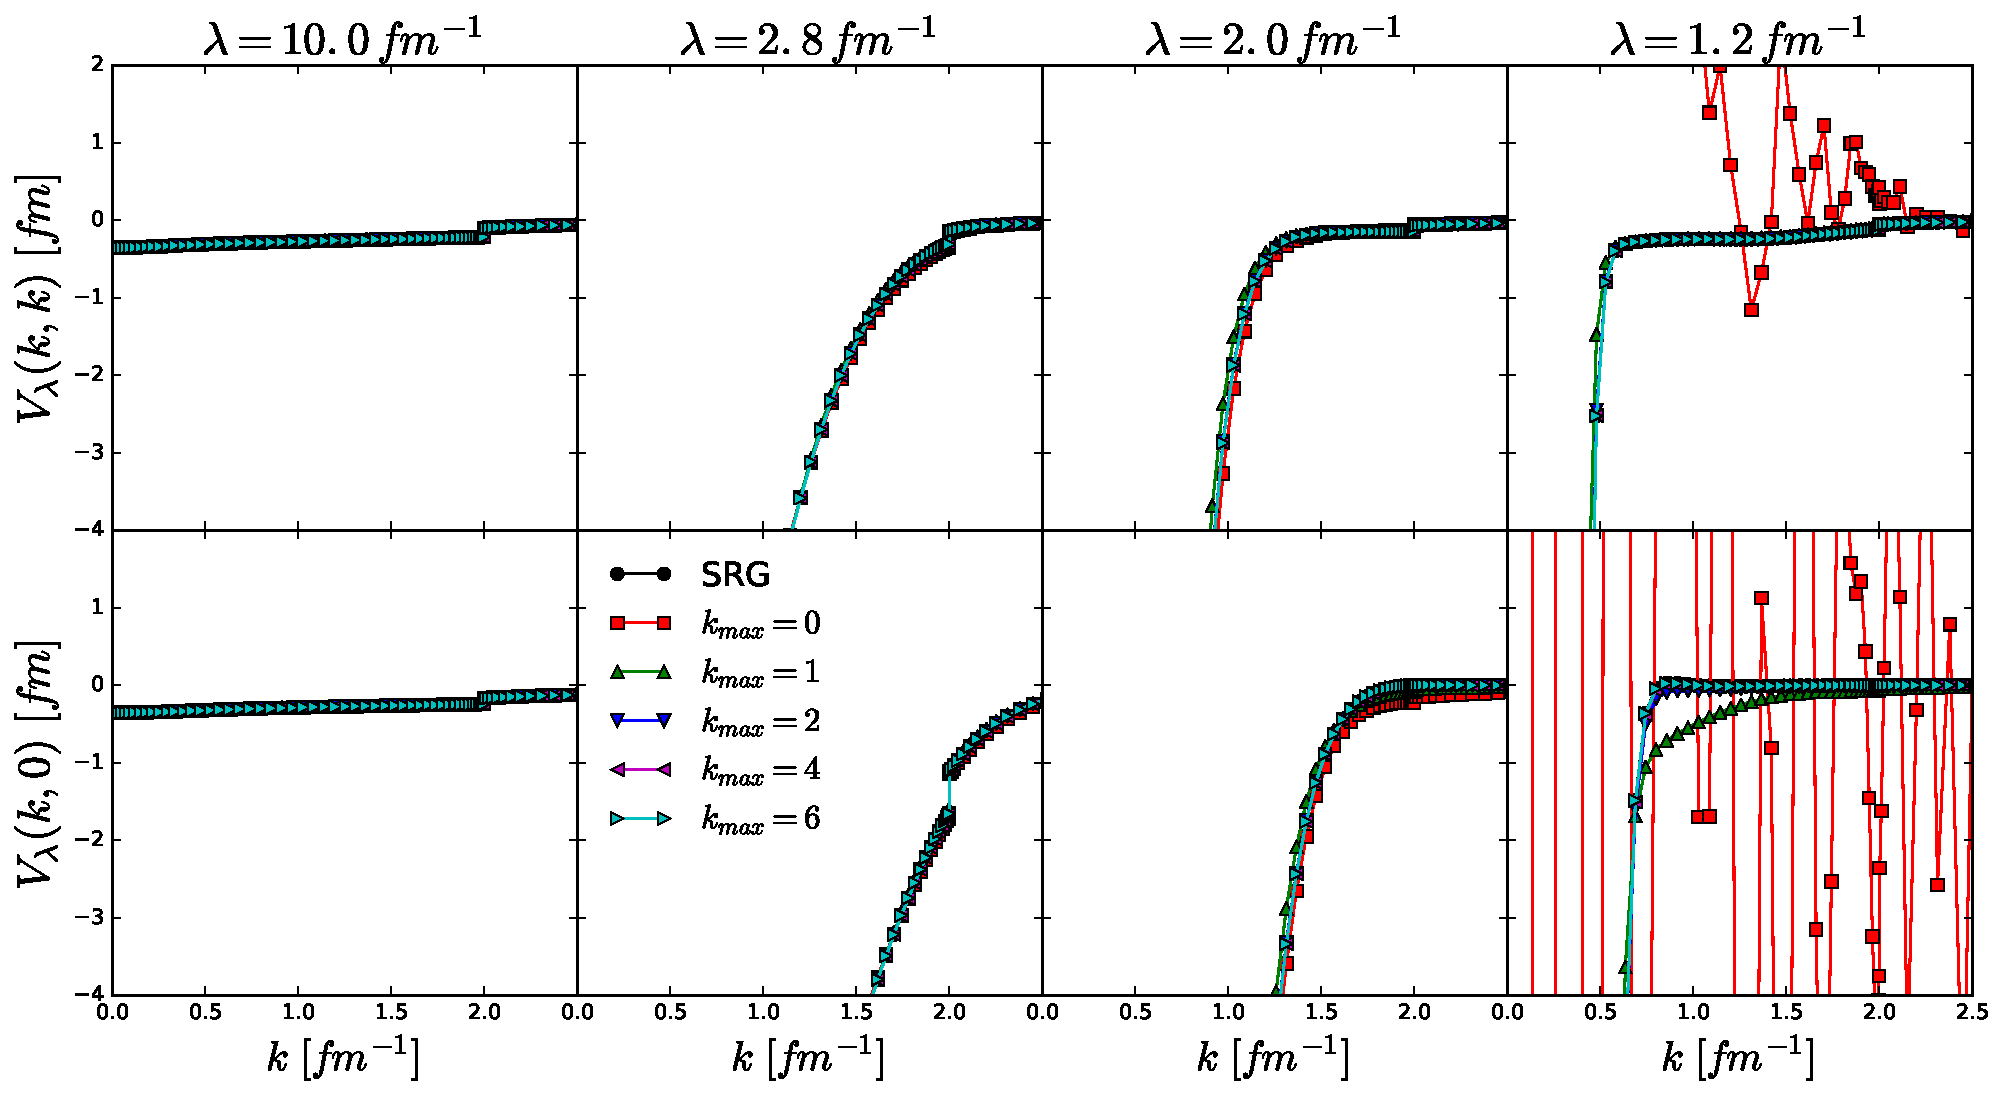
\includegraphics[width=15cm]{mag_diags_offdiags_RKE_4_Wilson}
   \hspace*{0.05\textwidth}%
  \caption{Diagonal and off-diagonal matrix elements of evolved $V_{\lambda}(k,k')$ with $G=T_{rel}$ and $\Lambda=4.0 \, fm^{-1}$ for several values of $\lambda$ and $k_{max}$ compared to the SRG result.}
  \label{fig:mag_diags_offdiags_RKE_4_Wilson}
\end{figure}

\newpage

%%%%%%%%%%%%%%%%%%%%%%%%%%%%%%%%%%%%%%%%%%%%%%%%%%%%%%%%%%%%%%%%%%%%%%%%%
\section{Work in progress}
\label{sec:future}

The Magnus expansion has trouble evolving potentials at very high cutoffs $\Lambda$, $20.0 \, fm^{-1}$ for the non-local potential and $9.0 \, fm^{-1}$ for the semi-local potential. For these cutoffs the size of $\Omega(s)$ increases drastically as $s$ is taken to larger values. (Note: this is independent of the step-size $ds$.) This leads to a numerical error in evaluating $e^{\Omega(s)}$ using either SciPy's expm function or the BCH formula. For this reason, we would like to understand the validity and convergence of the Magnus expansion and how this is affected by the cutoff. For all results in this section, $G=H_D$ and the non-local potential are used unless noted otherwise. \\

In Figure \ref{fig:omega_norms_Wendt_Wegner} we show the Frobenius norm of $\Omega(s)$ for three cutoffs $\Lambda$ and two extremes in $k_{max}$. This figure illustrates the problem as stated above: the size of $\Omega$ at high cutoffs leads to errors in matrix multiplication and exponentiation. At high $s$, the norm begins to flatten with the cutoffs of $4.0$ and $9.0 \, fm^{-1}$ allowing for a full evolution to $\lambda = 1.2 \, fm^{-1}$. However, with the cutoff of $20.0 \, fm^{-1}$, the norm jumps as $s \rightarrow 10^{-4}$. Notice that $||\Omega(s)||$ is generally independent of $k_{max}$, although at $\Lambda=20.0 \, fm^{-1}$ there is more sensitivity to $k_{max}$ with the larger truncation diverging first. Large $\Omega(s)$ leads to an increasing size from the nested commutator in the series in Eq. (\ref{eq:magnus_omega}).
%
\begin{figure}[H]
  \centering
  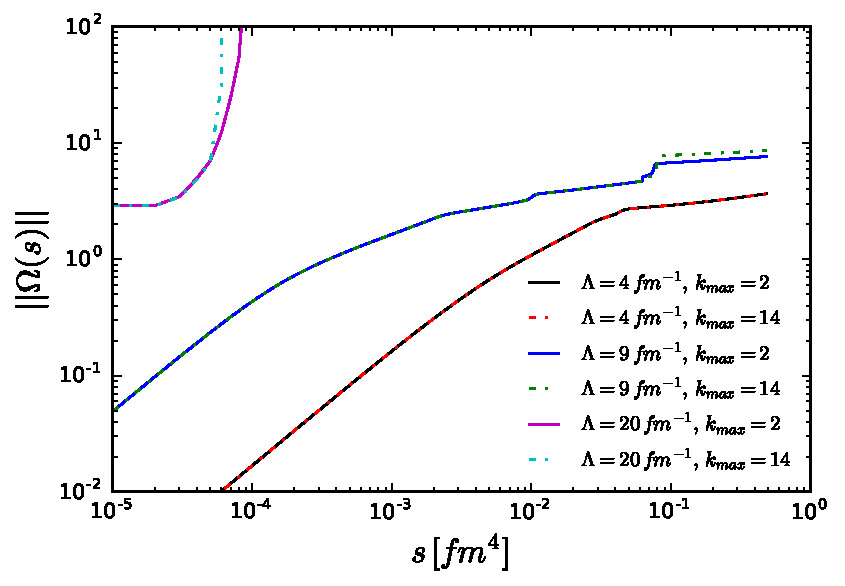
\includegraphics[width=10cm]{omega_norms_Wendt_Wegner}
   \hspace*{0.05\textwidth}%
  \caption{Frobenius norm of $\Omega(s)$ for $\Lambda = 4.0, \, 9.0,$ and $20.0 \, fm^{-1}$ and $k_{max}=2$ and $14$ as a function of $s$.}
  \label{fig:omega_norms_Wendt_Wegner}
\end{figure}
%
The convergence of the Magnus series depends on the SRG generator $\eta(s)$. In Figure \ref{fig:eta_norms_Wendt_Wegner} we plot the Frobenius norm of $\eta(s)$ for three cutoffs $\Lambda$ and two extremes in $k_{max}$ as before. We see that $||\eta(s)||$ decreases with $s$ for $\Lambda=4.0$ and $9.0 \, fm^{-1}$ but not for $\Lambda=20.0 \, fm^{-1}$. For this last case, the size of $\eta(s)$ increases up until $\lambda \sim 10.0 \, fm^{-1}$ until an error in expm is reached (where the two curves end). Also, it is not clear what causes the spike in $||\eta(s)||$ for $\Lambda=9.0 \, fm^{-1}$ at $s \sim 10^{-1}$. Checking this more closely, the spike occurs at $\lambda \approx 2.0 \, fm^{-1}$.
%
\begin{figure}[H]
  \centering
  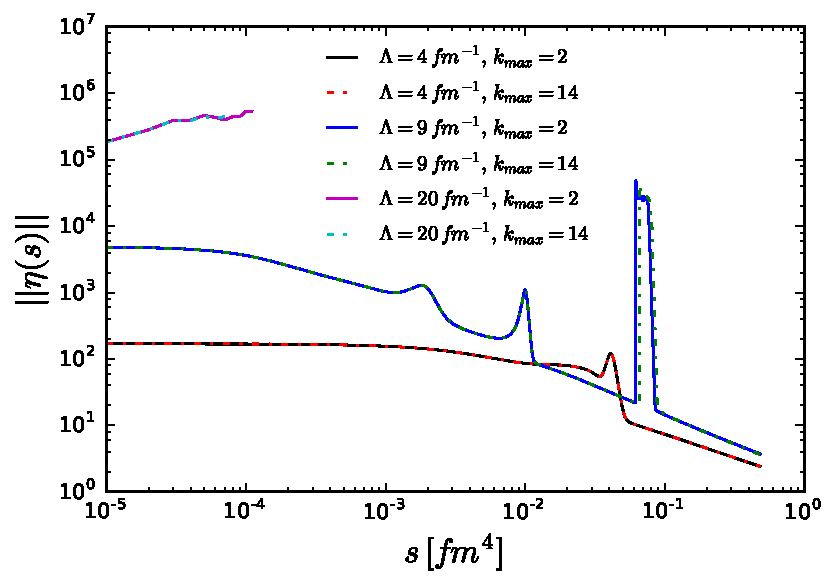
\includegraphics[width=10cm]{eta_norms_Wendt_Wegner}
   \hspace*{0.05\textwidth}%
  \caption{Frobenius norm of $\eta(s)$ for $\Lambda = 4.0, \, 9.0,$ and $20.0 \, fm^{-1}$ and $k_{max}=2$ and $14$ as a function of $s$.}
  \label{fig:eta_norms_Wendt_Wegner}
\end{figure}
%
\begin{table}[H]
\caption{Values of $\int_{0}^{s_{max}} ||\eta(s)|| ds$ for various values in $\Lambda$ and $k_{max}$. If the full evolution is not reached ($\lambda = 1.2 \, fm^{-1}$) because of a numerical error, then we report the last value of $\lambda$.}
\label{tab:convergence_integral}
\begin{ruledtabular}
\begin{tabular}{{>{\centering\arraybackslash}m{1.5in}>{\centering\arraybackslash}m{1.5in}>{\centering\arraybackslash}m{1.5in}>{\centering\arraybackslash}m{1.5in}}}
  $\Lambda \, [fm^{-1}]$ & $k_{max}$ & $\lambda \, [fm^{-1}]$ & $\int_{0}^{s_{max}} ||\eta(s)|| ds$ \\
  \colrule
  $4.0$ & $2$ & $1.2$ & $6.0119$ \\
  $4.0$ & $14$ & $1.2$ & $6.0195$ \\
  $9.0$ & $2$ & $1.2$ & $422.5080$ \\
  $9.0$ & $14$ & $1.2$ & $401.1647$ \\
  $20.0$ & $2$ & $9.7645$ & $43.8078$ \\
  $20.0$ & $14$ & $10.9327$ & $24.3842$ \\
\end{tabular}
\end{ruledtabular}
\end{table}

\newpage

% .....................................................................................................................................................................................................................................
\subsection{Convergence of the Magnus expansion}

As argued in \cite{Blanes:2009}, the size of $||\eta(s)||$ controls the convergence of the Magnus series. The value $\int_{0}^{s_{max}} ||\eta(s)|| ds$ provides a measure of how the Magnus expansion convergences, and thus gives a method to evaluate the validity of the expansion. In Table \ref{tab:convergence_integral} we provide several values of $\int_{0}^{s_{max}} ||\eta(s)|| ds$ for the various cases in $\Lambda$ and $k_{max}$. This reaffirms that the Magnus series diverges at higher cutoffs in $\Lambda$. The size of $\eta(s)$ becomes too large which accounts for the increasing size of $\Omega(s)$ leading to a numerical breakdown. In Table \ref{tab:convergence_integral} we provide the last value of $\lambda$ before an error occurs (only for $\Lambda = 20.0 \, fm^{-1}$). \\

There are a couple of important things to note in understanding this issue. One, the breakdown of the Magnus implementation is independent of the ODE solver. Using a built-in Python ODE solver (such as odeint), we recover the same error as with the Euler method. This implies that the ODE error on $\Omega(s)$ is the not the cause of the problem. Two, the large size of $\Omega(s)$ leads to problems with higher truncations and adaptive truncation methods in the Magnus expansion. Again, this is because the nested commutator in Eq. (\ref{eq:magnus_omega}) begins to grow in size leading to a numerical breakdown at lower values of $s$ than with the lower truncations. \\

In \cite{Blanes:2009}, Blanes argued that the Magnus expansion is convergent in the interval $s \in [0, \, T]$ where
%
\begin{eqnarray}
\label{eq:convergence_integral}
T = max \left \{ s \geq 0 \, : \, \int_{0}^{s} ||\eta(s')|| ds' \, < r_c \right \}.
\end{eqnarray}
%
The value of $r_c$ is debated but the consensus seems to be that $r_c = \pi$ (see \cite{Blanes:2009} for details). Nevertheless, this is a useful quantity to calculate for different cases in $\Lambda$ and $k_{max}$. In Figure \ref{fig:T_values_Wendt_Wegner} we show values of $T$ for the same cases as before with $r_c = \pi$. Note that in Eq. (\ref{eq:convergence_integral}) we use the flow parameter $s$, but in Figure \ref{fig:T_values_Wendt_Wegner} $T$ is given as a $\lambda$ value. A lower $T$ value in the figure means a further evolution can be safely reached. It is not surprising then that the $T$ values increase with $\Lambda$. Note that $T$ never drops below $2 \, fm^{-1}$ for any of the cases.

\newpage

%
\begin{figure}[H]
  \centering
  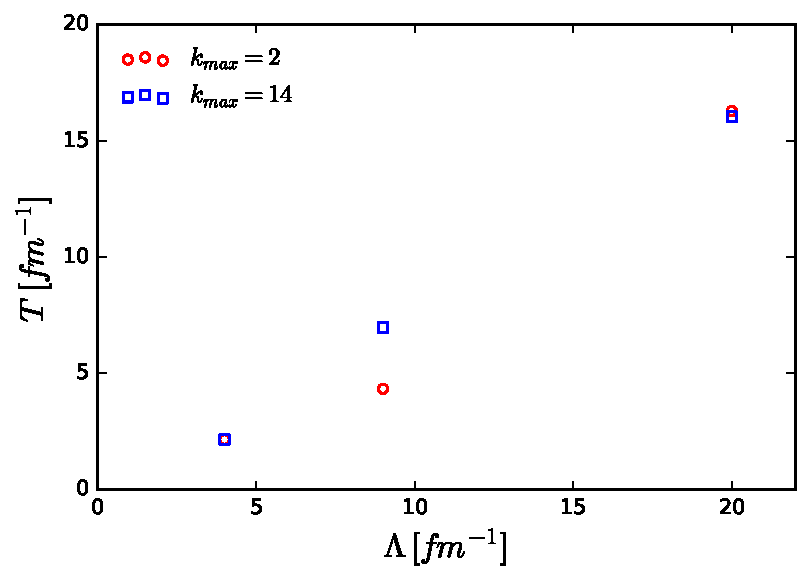
\includegraphics[width=10cm]{T_values_Wendt_Wegner}
   \hspace*{0.05\textwidth}%
  \caption{$T$ in units $fm^{-1}$ for $r_c=\pi$, $\Lambda = 4.0, \, 9.0,$ and $20.0 \, fm^{-1}$, and $k_{max}=2$ and $14$.}
  \label{fig:T_values_Wendt_Wegner}
\end{figure}
%
\begin{figure}[H]
  \centering
  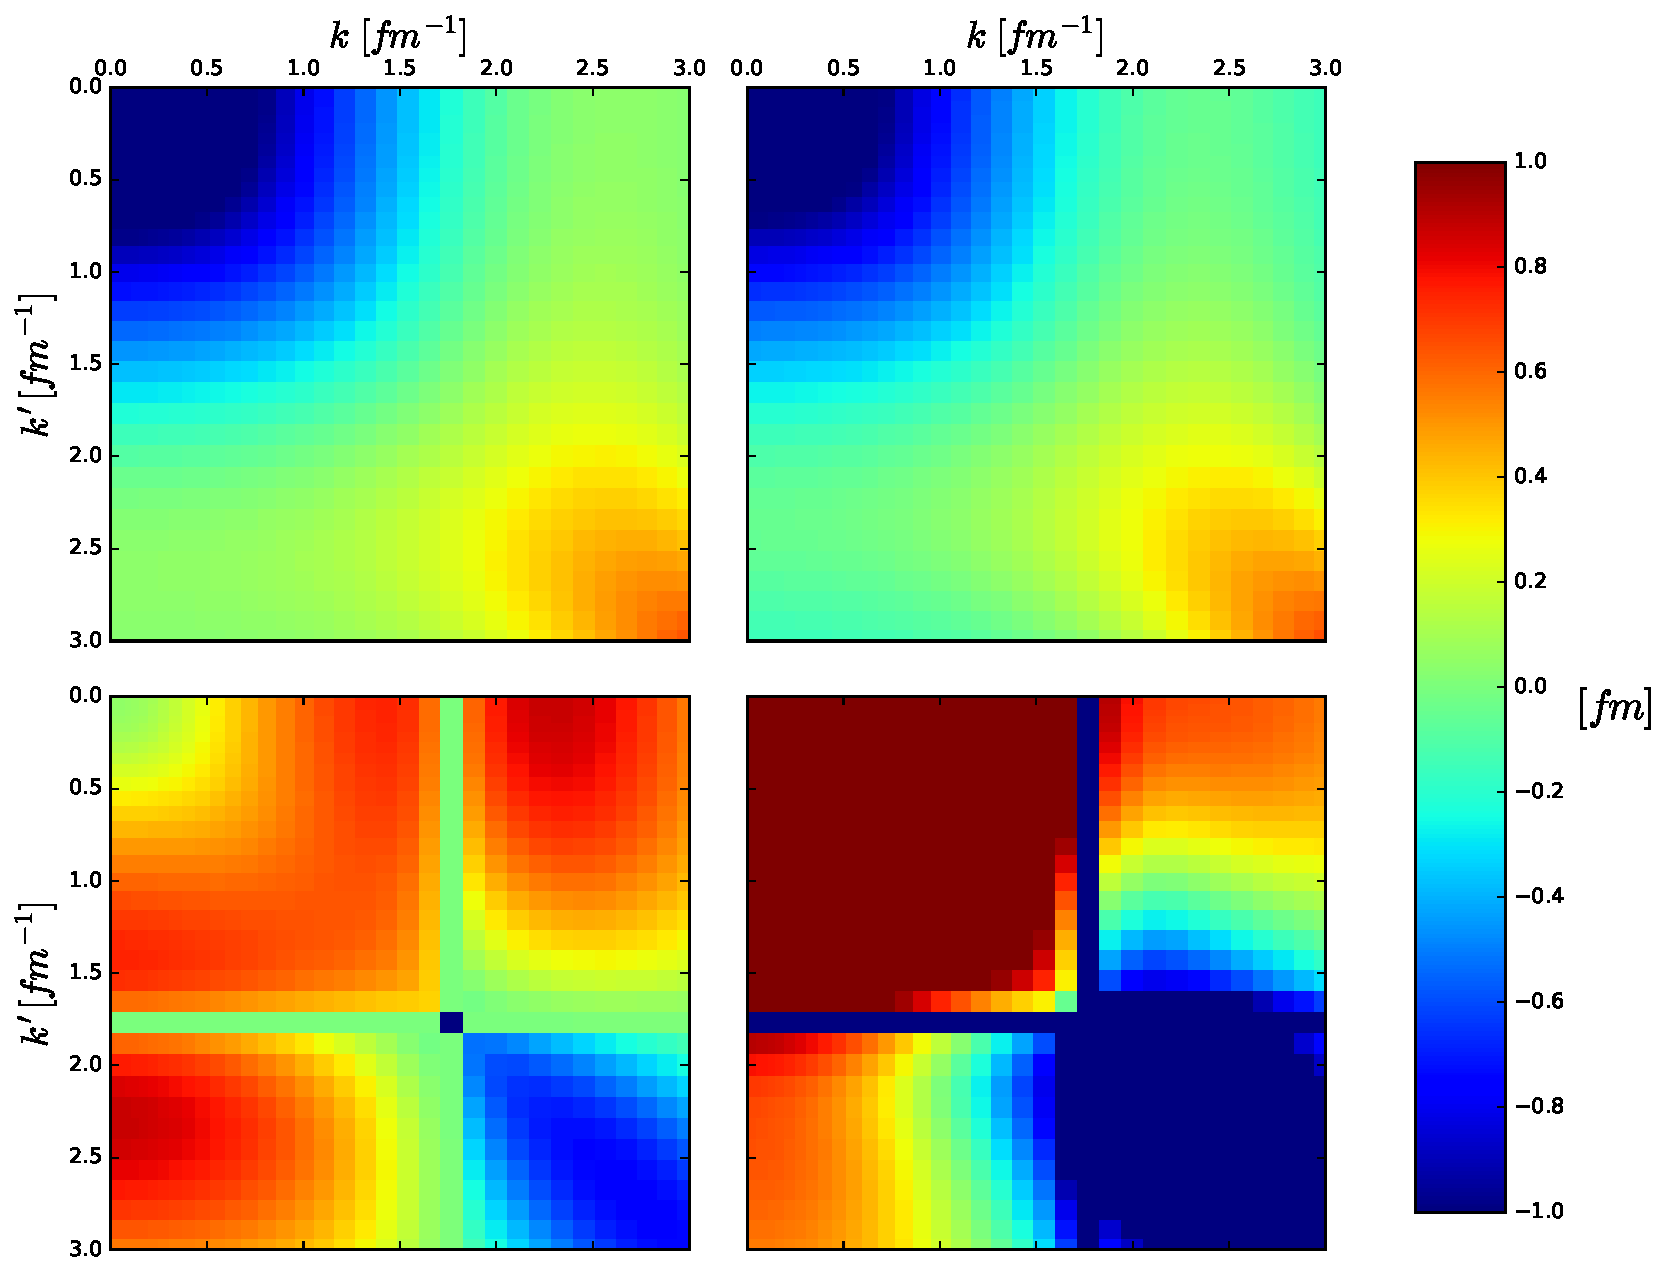
\includegraphics[width=15cm]{srg_gen_with_magnus_Wendt}
   \hspace*{0.05\textwidth}%
  \caption{Contour of evolved $V_{\lambda}(k,k')$ with $\Lambda=4.0\,fm^{-1}$ (top) and $\Lambda=9.0\,fm^{-1}$ (bottom) for the typical SRG approach (left) and the Magnus approach with $\eta^{SRG}(s)$ (right). Here $\lambda = 2.8 \, fm^{-1}$, $G=H_{D}$, and $k_{max}=6$.}
  \label{fig:srg_gen_with_magnus_Wendt}
\end{figure}
%
Another way to illustrate the problem is by using the SRG $\eta(s)$ for the Magnus expansion. In an ideal situation, the Magnus implementation matches the SRG approach exactly, and the use of the SRG $\eta(s)$ would not change the evolution in the Magnus implementation. We test this by SRG evolving, saving $\eta^{SRG}(s)$, and using this generator in Eq. (\ref{eq:magnus_omega}) for the Magnus evolution. We show $V_{\lambda}(k,k')$ evolved out to $\lambda=2.8 \, fm^{-1}$ with the typical SRG approach and Magnus implementation with the SRG generator for two cutoffs in Figure \ref{fig:srg_gen_with_magnus_Wendt}. The evolved potentials are almost identical at the lower cutoff of $4.0 \, fm^{-1}$ which is expected if everything in the Magnus implementation is working correctly. However, at the larger cutoff, there is a substantial difference in the evolution. This is a confusing result given that in Figure \ref{fig:mag_contours_Wendt_9_Wegner} we see good agreement between the SRG and $k_{max}=6$ Magnus. If anything, this shows that the SRG generator is not consistent between both approaches at high cutoffs, albeit a similar flow can be reached. \\

\textcolor{red}{Try more cutoffs $\Lambda$ using Epelbaum code} (chiraln3lo.f90) \cite{Epelbaum:2005}. \textcolor{red}{Step one: reproduce Wendt files.}

% .....................................................................................................................................................................................................................................
\subsection{Reducing the matrix size with decoupling}

As mentioned before, the SRG decouples the potential as it evolves in $s$. The low-momentum part of $V_s(k,k')$ is less sensitive to the high-momentum part as it evolves. From a practical standpoint, this can simplify calculations by pairing down the size of the matrix and removing high-momentum pieces. Here we try pairing down the matrix size as the potential evolves to hopefully improve the validity of the Magnus expansion. \\

First we consider $\Lambda = 9.0 \, fm^{-1}$. The method in pairing down the size of the matrices in the Magnus implementation is as follows: if $\frac{||H_{OD}(s_{i})||}{||H_{OD}(s_{j})||} < R$ where the indices i and j represent the latest step in the Euler method and the last index in which the ratio is less than $R$ respectively, then we pair down the size of $H(s)$ sub-blocks and restart the ODE solver. We choose the value of $R$ such that the matrices are reduced in a stable manner. We test three different criteria for this method and compare to the normal result from before. In Table \ref{tab:reduced_matrix_method_table} and Figures \ref{fig:reduced_matrix_omega_norms_V9}, \ref{fig:reduced_matrix_eta_norms_V9}, and \ref{fig:reduced_matrix_mag_diff_V9} we show results for these criteria with $k_{max}=6$, $G=H_D$, and $ds=10^{-5}$.
%
\begin{table}[H]
\caption{Values of the final Hamiltonian matrix size, $N$, and $\int_{0}^{s_{max}} ||\eta(s)|| ds$ for various methods in pairing down the matrix size and values in $\lambda$. Here the cut size is the integer in which each sub-block of the Hamiltonian is reduced once the condition $\frac{||H_{OD}(s_{i})||}{||H_{OD}(s_{j})||} < R$ is met. The first three rows show the results for the original, uncut Hamiltonian.}
\label{tab:reduced_matrix_method_table}
\begin{ruledtabular}
\begin{tabular}{{>{\centering\arraybackslash}m{1in}>{\centering\arraybackslash}m{1in}>{\centering\arraybackslash}m{1in}>{\centering\arraybackslash}m{1in}>{\centering\arraybackslash}m{1in}}}
  Cut size & $R$ & $\lambda \, [fm^{-1}]$ & $N$ & $\int_{0}^{s_{max}} ||\eta(s)|| ds$ \\
  \colrule
   & & $2.8$ & $240$ & $6.9327$ \\
  $0$ & $0$ & $2.0$ & $240$ & $8.6020$ \\
   & & $1.2$ & $240$ & $440.8445$ \\ \hline
   & & $2.8$ & $200$ & $6.9327$ \\
   $5$ & $0.6$ & $2.0$ & $190$ & $8.6020$ \\
   & & $1.2$ & $180$ & $326.4978$ \\ \hline
   & & $2.8$ & $180$ & $6.9327$ \\
   $10$ & $0.5$ & $2.0$ & $180$ & $8.6020$ \\
   & & $1.2$ & $160$ & $11.7170$ \\ \hline
   & & $2.8$ & $180$ & $6.9327$ \\
   $15$ & $0.4$ & $2.0$ & $180$ & $8.6020$ \\
   & & $1.2$ & $150$ & $11.7170$ \\
\end{tabular}
\end{ruledtabular}
\end{table}
%
In Figure \ref{fig:reduced_matrix_omega_norms_V9} we see that the size of the $\Omega(s)$ matrix is substantially reduced for the later two cases in pairing down the Hamiltonian. The troughs in the curve correspond to where the matrices are cut in size. We see large jumps in the original and first case matching the spike in $||\eta(s)||$ as seen in Figure \ref{fig:reduced_matrix_eta_norms_V9}. Note that this spike is absent for the later two cases which keeps the value of $\int_{0}^{s_{max}} ||\eta(s)|| ds$ relatively low in comparison. \\

In Figure \ref{fig:reduced_matrix_mag_diff_V9} we show the absolute difference in the diagonal and off-diagonal matrix elements of $V_{\lambda}(k,k')$ between the original SRG case and the Magnus, reduced matrix case. There is better agreement between the original SRG result and the reduced matrix cases than with the original Magnus result, even more so at $\lambda = 1.2 \, fm^{-1}$. This is an encouraging result as the reduced matrix method preserves the intended evolution. Lastly, we check the accuracy of the evolved eigenvalues and phase shifts with respect to the original Hamiltonian in Table \ref{tab:reduced_matrix_V9_errors}. We see that the evolved and paired down Hamiltonians keep high accuracy in the deuteron bound state energy although two orders of magnitude worse than the uncut Magnus evolution; however, there is some deviation from the uncut phase shifts seen in Figure \ref{fig:reduced_matrix_phase_shifts_V9}.
%
\begin{figure}[H]
  \centering
  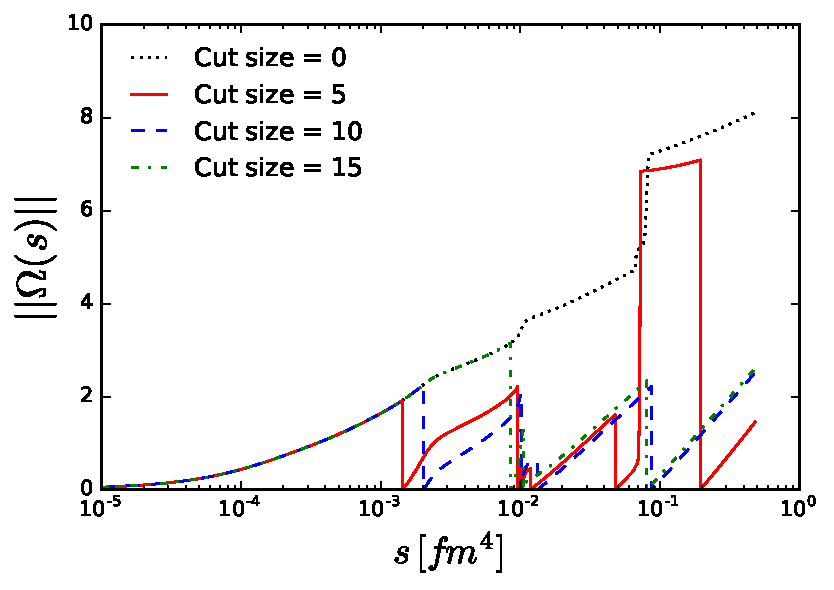
\includegraphics[width=10cm]{reduced_matrix_omega_norms_V9}
   \hspace*{0.05\textwidth}%
  \caption{Frobenius norm of $\Omega(s)$ for cut sizes of $0$, $5$, $10$, and $15$ and $R=0.0$, $0.6$, $0.5$, and $0.4$. Here $\Lambda=9.0 \, fm^{-1}$, $G=H_D$, and $k_{max}=6$.}
  \label{fig:reduced_matrix_omega_norms_V9}
\end{figure}
%
\begin{figure}[H]
  \centering
  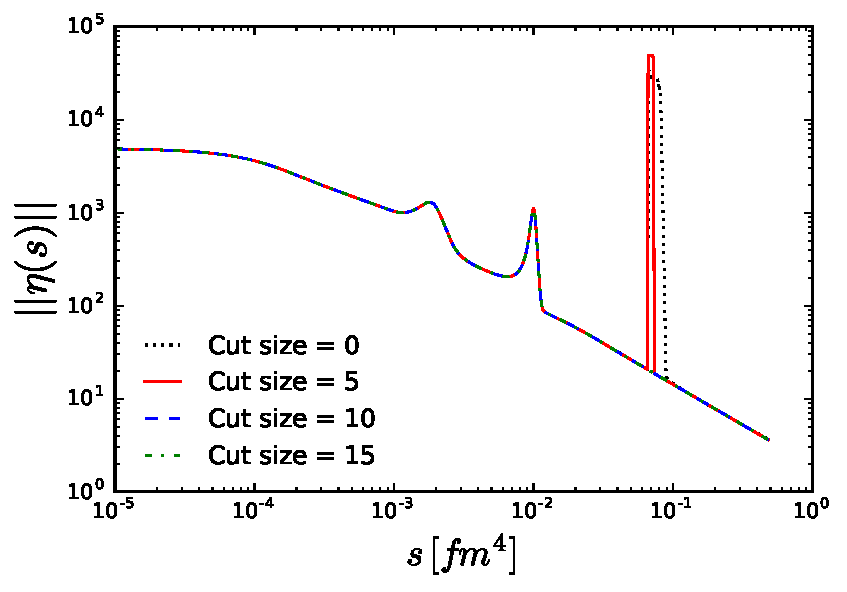
\includegraphics[width=10cm]{reduced_matrix_eta_norms_V9}
   \hspace*{0.05\textwidth}%
  \caption{Frobenius norm of $\eta(s)$ for cut sizes of $0$, $5$, $10$, and $15$ and $R=0.0$, $0.6$, $0.5$, and $0.4$. Here $\Lambda=9.0 \, fm^{-1}$, $G=H_D$, and $k_{max}=6$.}
  \label{fig:reduced_matrix_eta_norms_V9}
\end{figure}
%
\newpage
%
\begin{figure}[H]
  \centering
  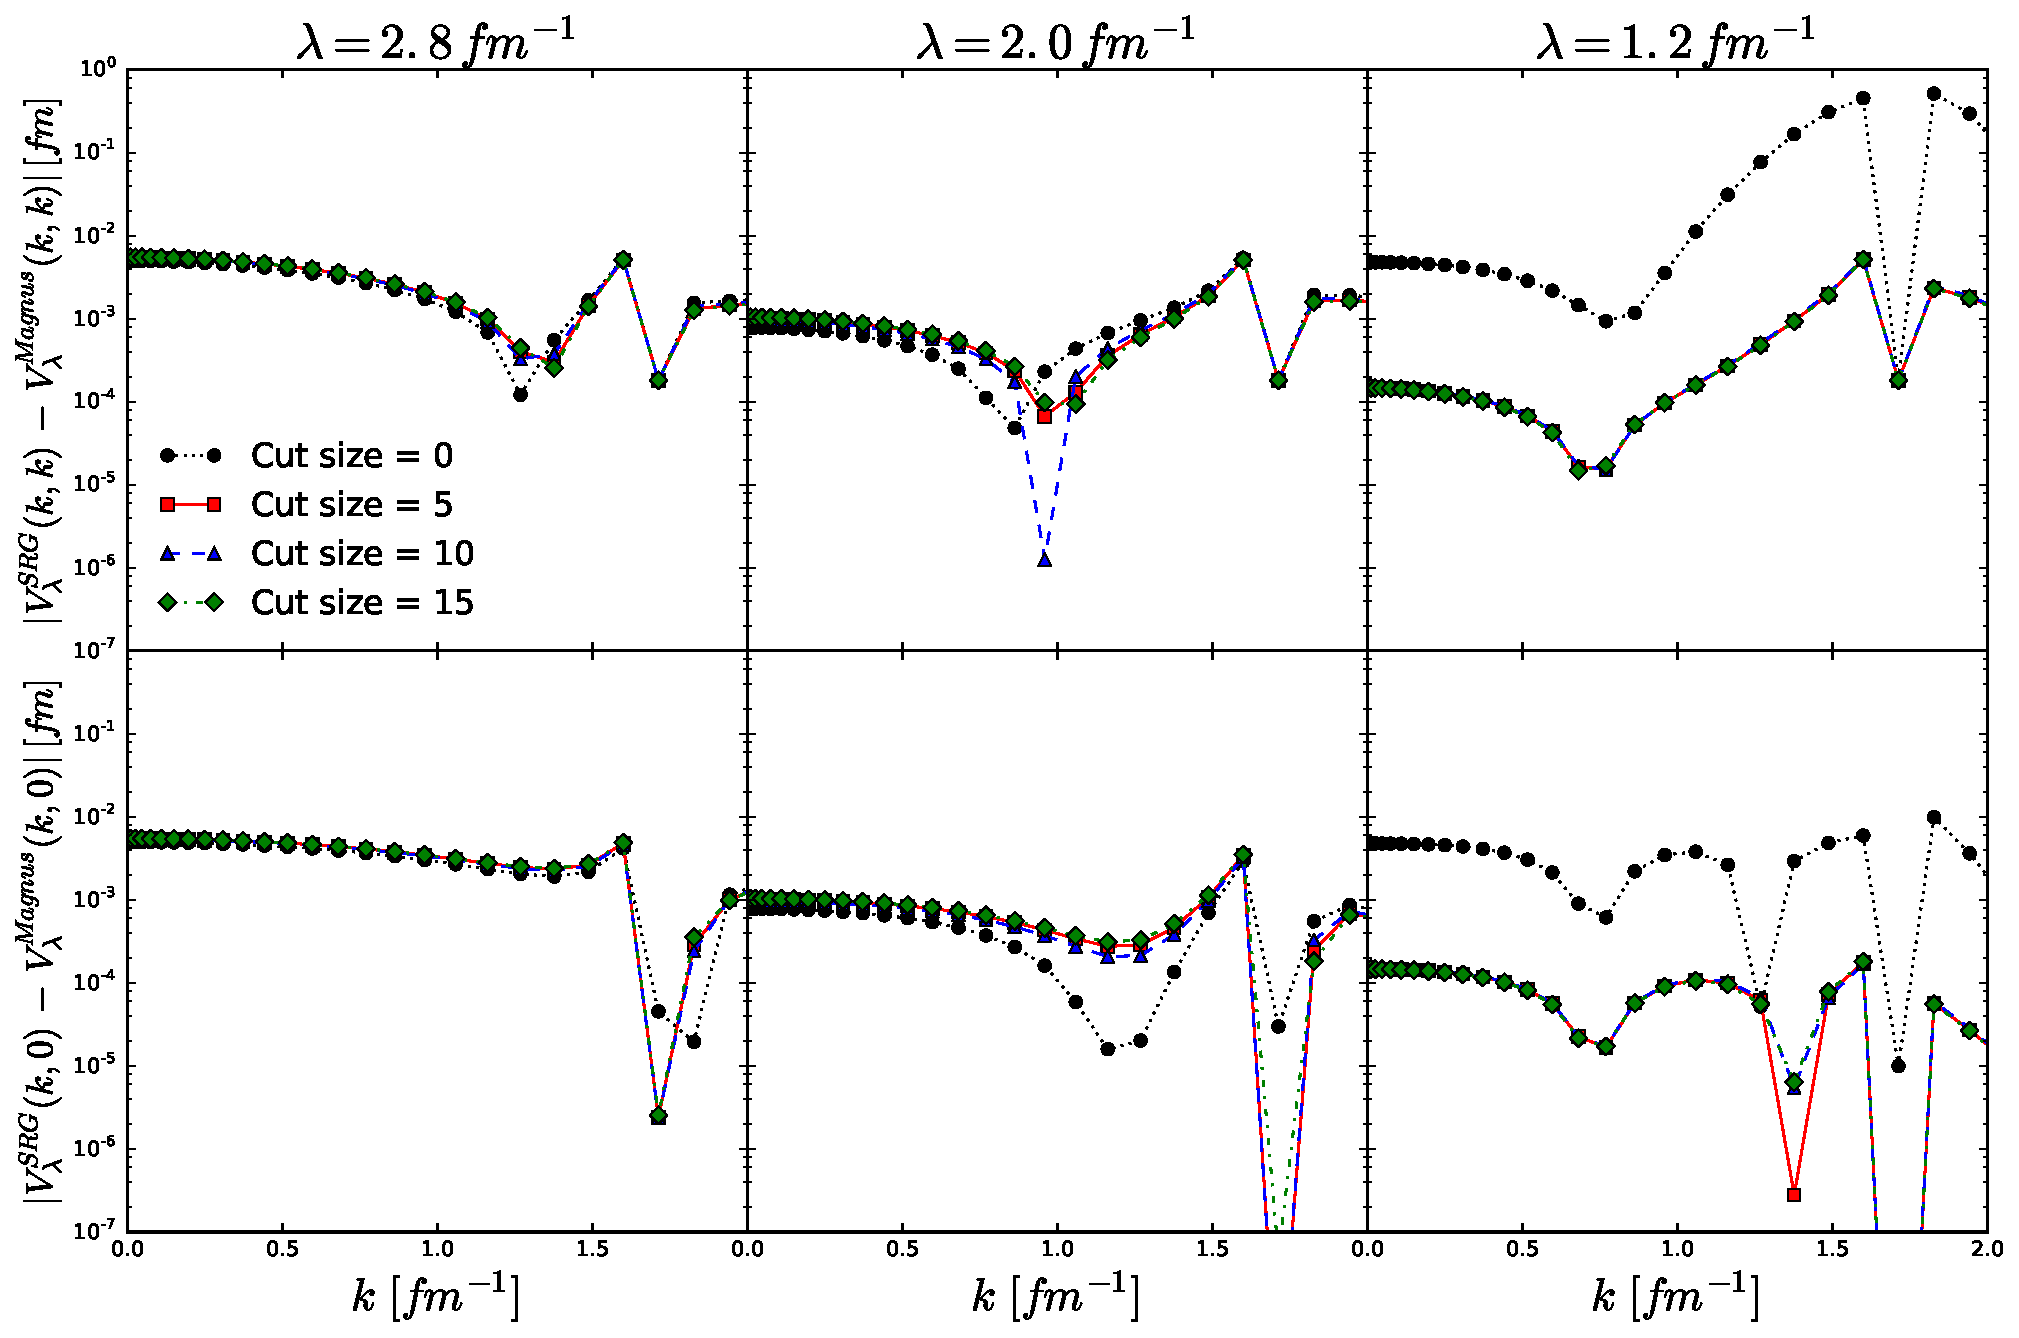
\includegraphics[width=15cm]{reduced_matrix_mag_diff_V9}
   \hspace*{0.05\textwidth}%
  \caption{Difference in the diagonal and off-diagonal matrix elements of evolved $V_{\lambda}(k,k')$ with cut sizes of $0$, $5$, $10$, and $15$ and $R=0.0$, $0.6$, $0.5$, and $0.4$. Here $\Lambda=9.0 \, fm^{-1}$, $G=H_D$, and $k_{max}=6$.}
  \label{fig:reduced_matrix_mag_diff_V9}
\end{figure}
%
\begin{figure}[H]
  \centering
  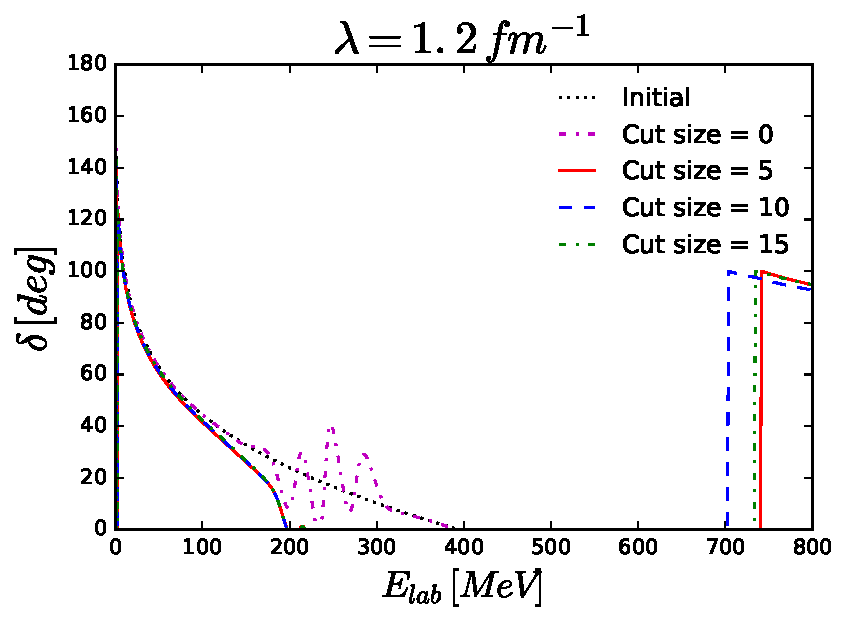
\includegraphics[width=10cm]{reduced_matrix_phase_shifts_V9}
   \hspace*{0.05\textwidth}%
  \caption{$^{3}S_{1}$ phase shifts for cut sizes of $0$, $5$, $10$, and $15$ and $R=0.0$, $0.6$, $0.5$, and $0.4$. Here $\Lambda=9.0 \, fm^{-1}$, $G=H_D$, and $k_{max}=6$.}
  \label{fig:reduced_matrix_phase_shifts_V9}
\end{figure}
%
\newpage
%
\begin{table}[H]
\caption{Relative error in the deuteron bound state energy where $\tilde{\epsilon}$ denotes an evolved eigenvalue with SRG and Magnus, reduced matrix evolved Hamiltonians for $\Lambda=9.0 \, fm^{-1}$ and $\lambda=1.2 \, fm^{-1}$.}
\label{tab:reduced_matrix_V9_errors}
\begin{ruledtabular}
\begin{tabular}{{>{\centering\arraybackslash}m{1in}>{\centering\arraybackslash}m{1in}>{\centering\arraybackslash}m{1in}>{\centering\arraybackslash}m{1in}>{\centering\arraybackslash}m{1in}}}
  $ $ & Cut size & $R$ & $N$ & $ |\frac{\epsilon_d-\tilde{\epsilon}_d}{\epsilon_d}| $ \\
  \colrule
  SRG & $0$ & $0.0$ & $240$ & $\num{2.428e-06}$ \\ \hline
  Magnus & $0$ & $0.0$ & $240$ & $\num{6.104e-13}$ \\
  Magnus & $5$ & $0.6$ & $180$ & $\num{8.781e-11}$ \\
  Magnus & $10$ & $0.5$ & $160$ & $\num{7.771e-11}$ \\
  Magnus & $15$ & $0.4$ & $150$ & $\num{3.727e-11}$ \\
\end{tabular}
\end{ruledtabular}
\end{table}
%
Next we consider $\Lambda = 20.0 \, fm^{-1}$. After testing this method to allow for a full Magnus evolution to $\lambda = 1.2 \, fm^{-1}$, we set $ds=10^{-6}$ and each $R$ value $0.2$ higher from before to ensure more cuts earlier in the flow. We keep the same number of terms in the Magnus expansion $k_{max} = 6$ and $G=H_D$. Recall that at this cutoff, we cannot fully evolve the uncut Hamiltonian. This is seen in Figure \ref{fig:reduced_matrix_omega_norms_V20} where $||\Omega(s)||$ diverges before fully evolving. Thus, the $||\eta(s)||$ curve in Figure \ref{fig:reduced_matrix_eta_norms_V20} for the uncut case ends before reaching the last value of $s$. Notice that early cuts in the Hamiltonian prevent $||\Omega(s)||$ from diverging. By removing the very high-momentum pieces of the Hamiltonian, we are able to achieve a full evolution in all three reduced matrix cases.
%
\begin{figure}[H]
  \centering
  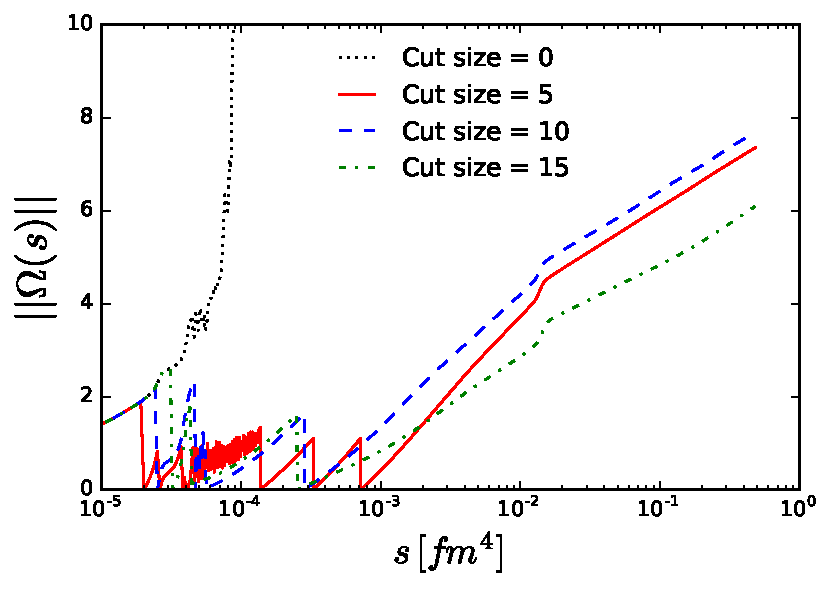
\includegraphics[width=10cm]{reduced_matrix_omega_norms_V20}
   \hspace*{0.05\textwidth}%
  \caption{Frobenius norm of $\Omega(s)$ for cut sizes of $0$, $5$, $10$, and $15$ and $R=0.0$, $0.8$, $0.7$, and $0.6$. Here $\Lambda=20.0 \, fm^{-1}$, $G=H_D$, and $k_{max}=6$.}
  \label{fig:reduced_matrix_omega_norms_V20}
\end{figure}
%
\begin{figure}[H]
  \centering
  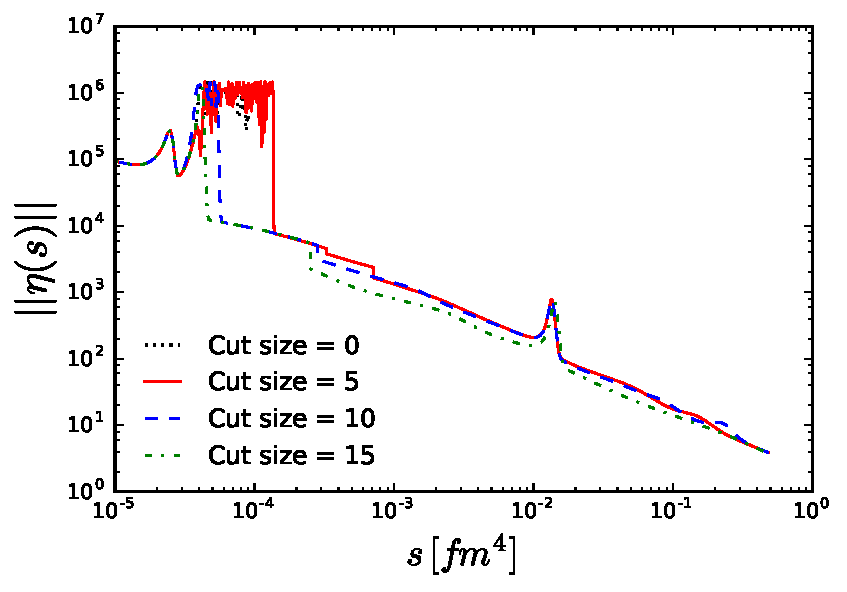
\includegraphics[width=10cm]{reduced_matrix_eta_norms_V20}
   \hspace*{0.05\textwidth}%
  \caption{Frobenius norm of $\eta(s)$ for cut sizes of $0$, $5$, $10$, and $15$ and $R=0.0$, $0.8$, $0.7$, and $0.6$. Here $\Lambda=20.0 \, fm^{-1}$, $G=H_D$, and $k_{max}=6$.}
  \label{fig:reduced_matrix_eta_norms_V20}
\end{figure}
%
\begin{figure}[H]
  \centering
  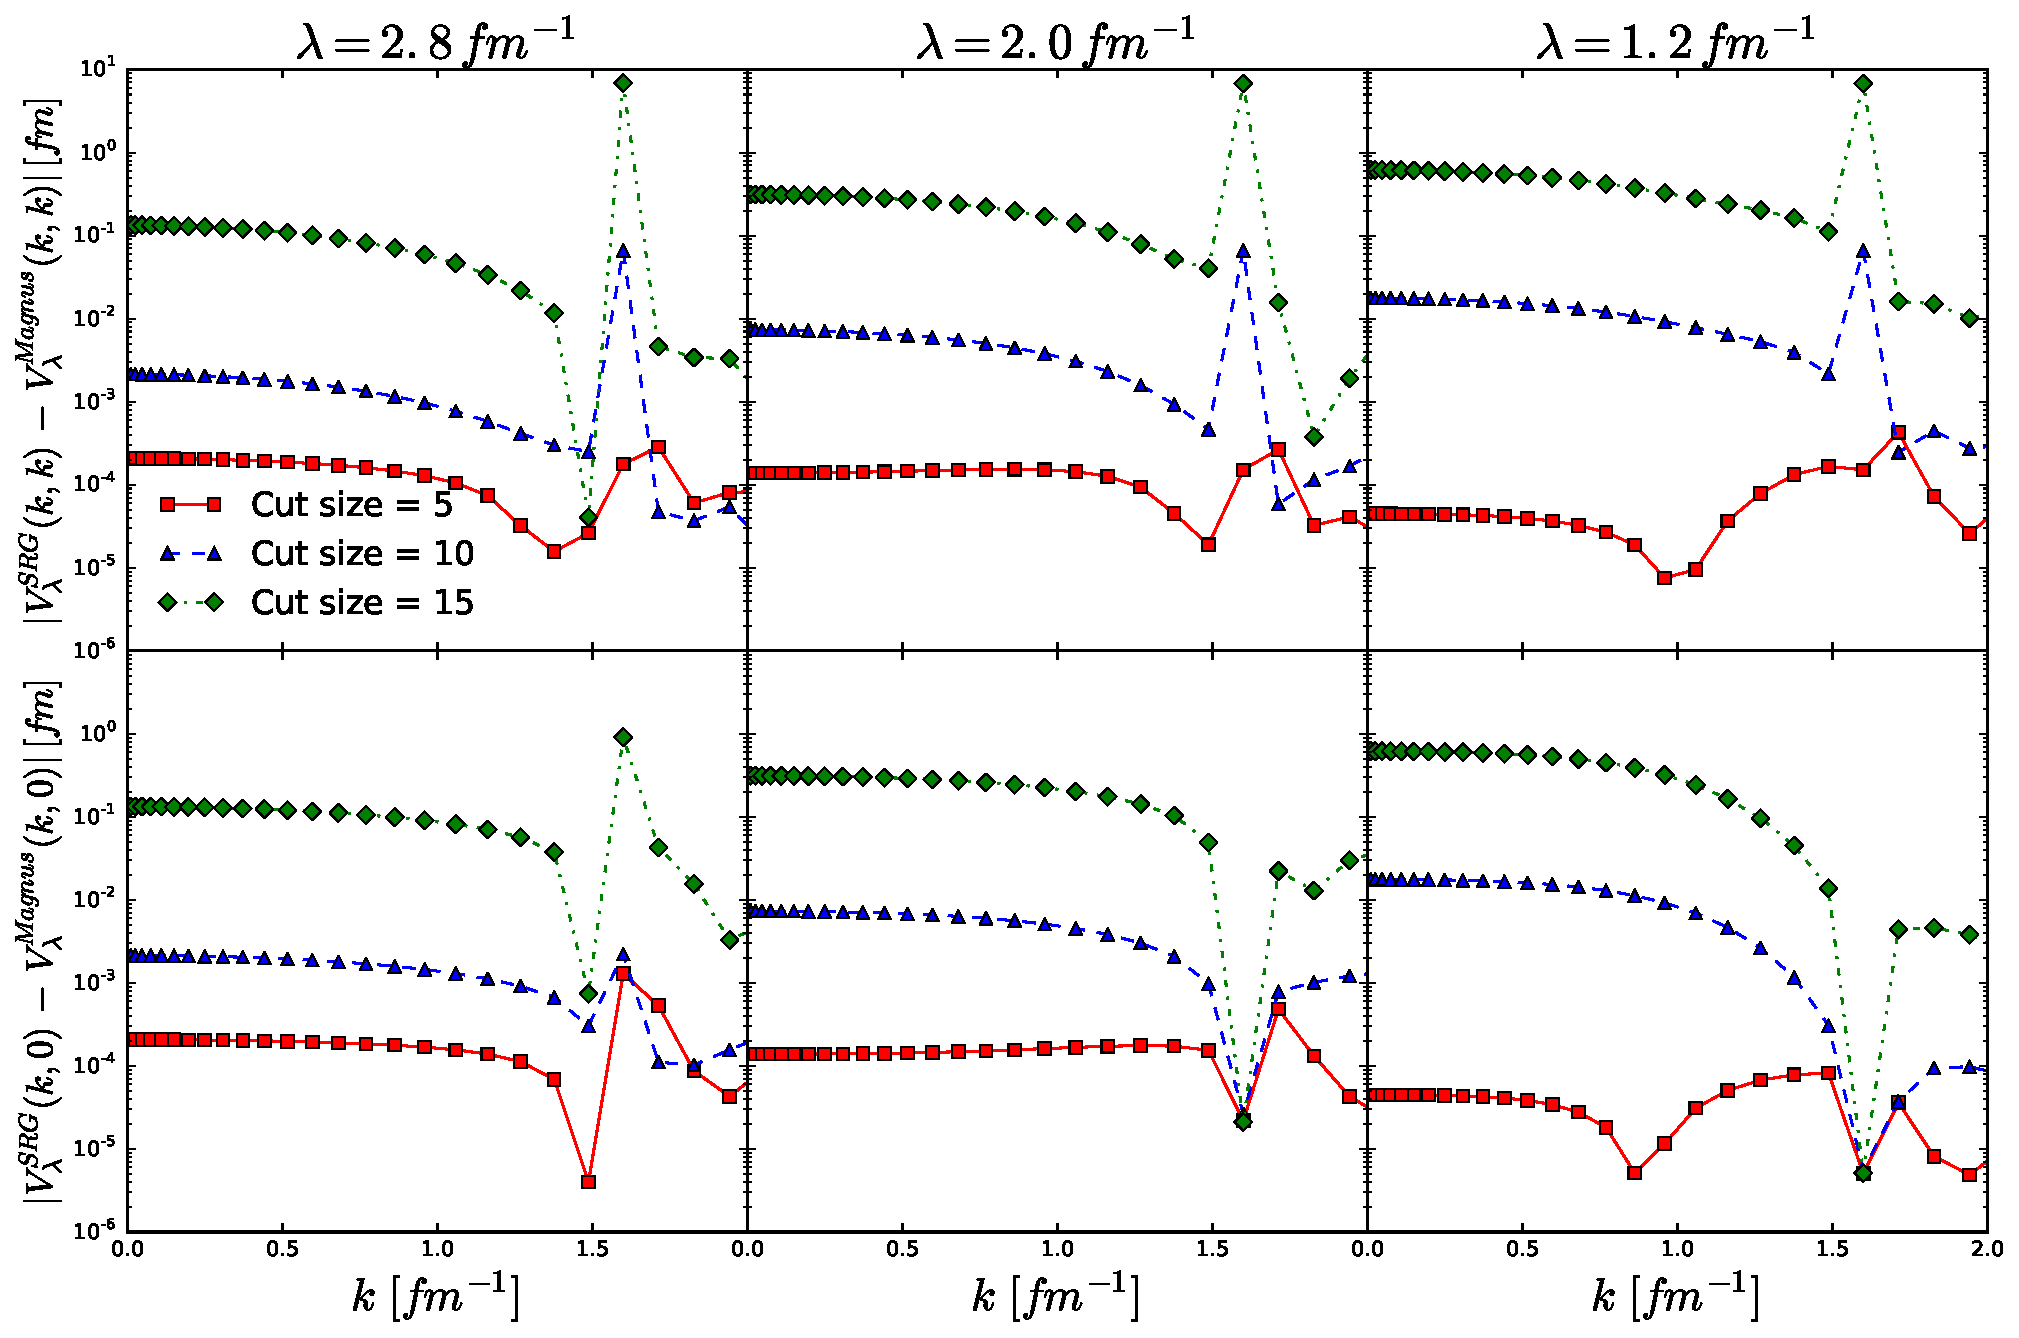
\includegraphics[width=15cm]{reduced_matrix_mag_diff_V20}
   \hspace*{0.05\textwidth}%
  \caption{Difference in the diagonal and off-diagonal matrix elements of evolved $V_{\lambda}(k,k')$ with cut sizes of $5$, $10$, and $15$ and $R=0.8$, $0.7$, and $0.6$. Here $\Lambda=20.0 \, fm^{-1}$, $G=H_D$, and $k_{max}=6$.}
  \label{fig:reduced_matrix_mag_diff_V20}
\end{figure}
%
The agreement with the SRG evolved result shows extreme sensitivity to the method in which the Hamiltonian is reduced. In Figure \ref{fig:reduced_matrix_mag_diff_V20}, we see that the choice of $R=0.8$ with a cut size of $5$ gives the best agreement with the SRG result for the evolved potential. This is reinforced by checking the accuracy on the deuteron bound state energy (Table \ref{tab:reduced_matrix_V9_errors}) where this case also shows the best agreement with the original, un-evolved Hamiltonian. Unlike with the lower cutoff of $\Lambda = 9.0 \, fm^{-1}$, the deuteron bound state is affected significantly with the Hamiltonian being paired down early in the flow equation suggesting that we are removing information at high-momentum that is not quite decoupled from the low-momentum. The phase shifts also show more sensitivity to the larger cut size of 15 whereas cut sizes of 5 and 10 keep the deviation consistent with the results for $\Lambda = 9.0 \, fm^{-1}$.
%
\begin{table}[H]
\caption{Relative error in the deuteron bound state energy where $\tilde{\epsilon}$ denotes an evolved eigenvalue with SRG and Magnus, reduced matrix evolved Hamiltonians for $\Lambda=20.0 \, fm^{-1}$ and $\lambda=1.2 \, fm^{-1}$.}
\label{tab:reduced_matrix_V20_errors}
\begin{ruledtabular}
\begin{tabular}{{>{\centering\arraybackslash}m{1in}>{\centering\arraybackslash}m{1in}>{\centering\arraybackslash}m{1in}>{\centering\arraybackslash}m{1in}>{\centering\arraybackslash}m{1in}}}
  $ $ & Cut size & $R$ & $N$ & $ |\frac{\epsilon_d-\tilde{\epsilon}_d}{\epsilon_d}| $ \\
  \colrule
  SRG & $0$ & $0.0$ & $240$ & $\num{5.869e-06}$ \\ \hline
  Magnus & $5$ & $0.8$ & $160$ & $\num{3.651e-05}$ \\
  Magnus & $10$ & $0.7$ & $160$ & $\num{3.114e-02}$ \\
  Magnus & $15$ & $0.6$ & $150$ & $\num{8.211e-01}$ \\
\end{tabular}
\end{ruledtabular}
\end{table}
%
\begin{figure}[H]
  \centering
  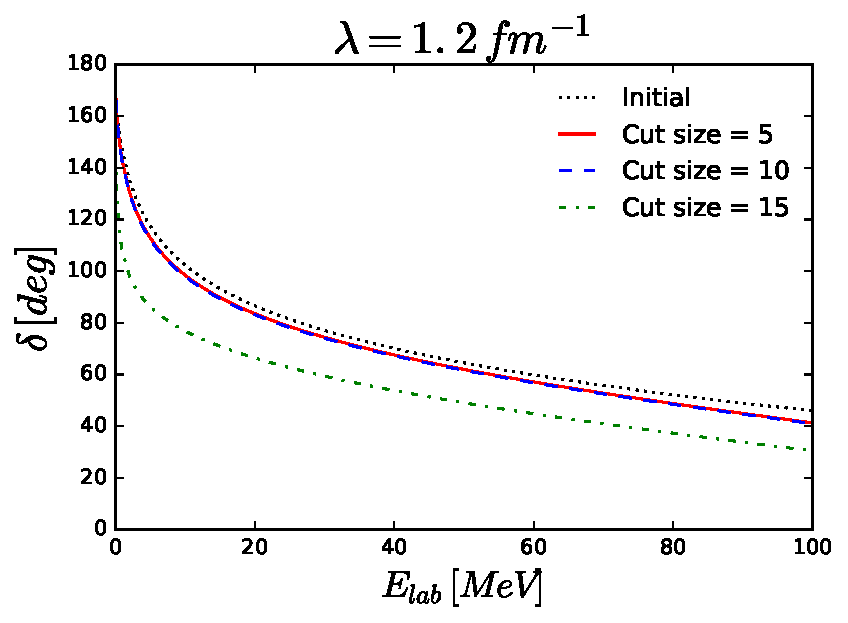
\includegraphics[width=10cm]{reduced_matrix_phase_shifts_V20}
   \hspace*{0.05\textwidth}%
  \caption{$^{3}S_{1}$ phase shifts for cut sizes $5$, $10$, and $15$ and $R=0.8$, $0.7$, and $0.6$. Here $\Lambda=20.0 \, fm^{-1}$, $G=H_D$, and $k_{max}=6$.}
  \label{fig:reduced_matrix_phase_shifts_V20}
\end{figure}
%
\textcolor{red}{Other ideas: Smooth cutoff on matrices. Try evolving different operators.}

%%%%%%%%%%%%%%%%%%%%%%%%%%%%%%%%%%%%%%%%%%%%%%%%%%%%%%%%%%%%%%%%%%%%%%%%%
\begin{thebibliography}{99}

\bibitem{Hergert:2017}
H.~Hergert, S.~K.~Bogner, J.~G.~Lietz, T.~D.~Morris, S.~Novario, N.~M.~Parzuchowski, and F.~Yuan,
Lect. Notes Phys. {\bf 936}, 477 (2017).

\bibitem{Wegner:1994}
F.~Wegner,
Ann. Phys. (Leipzig) {\bf 3}, 77 (1994).

\bibitem{Morris:2015}
T.~D.~Morris, N.~M.~Parzuchowski, and S.~K.~Bogner,
Phys. Rev. C {\bf 92}, 034331 (2015).

\bibitem{Glazek:2008}
S.~D.~Glazek and R.~J.~Perry,
Phys. Rev. D {\bf 78}, 045011 (2008).

\bibitem{Wendt:2011}
K.~A.~Wendt, R.~J.~Furnstahl, and R.~J.~Perry,
Phys. Rev. C {\bf 83}, 034005 (2011).

\bibitem{Magnus:1954}
W.~Magnus,
Communications on Pure and Applied Mathematics {\bf 7}, 649 (1954).

\bibitem{Blanes:2009}
S.~Blanes, F.~Casas, J.~Oteo, and J.~Ros,
Physics Reports {\bf 470}, 151 (2009).

\bibitem{Parzuchowski:2017}
N.~M.~Parzuchowski, S.~R.~Stroberg, P.~Navr{\'a}til, H.~Hergert, and S.~K.~Bogner,
Phys. Rev. C {\bf 96}, 034324 (2017).

\bibitem{Nogga:2005}
A.~Nogga, R.~G.~E. Timmermans, and U.~van~Kolck,
Phys. Rev. C {\bf 72}, 054006 (2005).

\bibitem{Bogner:2007}
S.~K.~Bogner, R.~J.~Furnstahl, and R.~J.~Perry,
Phys. Rev. C {\bf 75}, 061001(R) (2007).

\bibitem{Bogner:2010}
S.~K.~Bogner, R.~J.~Furnstahl, and A.~Schwenk,
Prog. Part. Nucl. Phys. {\bf 65}, 94 (2010).

\bibitem{Reinert:2018}
P.~Reinert, H.~Krebs, and E.~Epelbaum,
Eur. Phys. J. A {\bf 54}, 86 (2018).

\bibitem{Epelbaum:2005}
E.~Epelbaum, W.~Gl{\"o}ckle, and U.-G.~Mei{\ss}ner,
Nucl. Phys. A {\bf 747}, 362 (2005).

\end{thebibliography}

\end{document}